\documentclass[a4paper]{article}

\def\npart {II}
\def\nterm {Lent}
\def\nyear {2016}
\def\nlecturer {I. Grojnowski}
\def\ncourse {Number Fields}

% Imports
\ifx \nextra \undefined
  \usepackage[pdftex,
    hidelinks,
    pdfauthor={Dexter Chua},
    pdfsubject={Cambridge Maths Notes: Part \npart\ - \ncourse},
    pdftitle={Part \npart\ - \ncourse},
  pdfkeywords={Cambridge Mathematics Maths Math \npart\ \nterm\ \nyear\ \ncourse}]{hyperref}
  \title{Part \npart\ - \ncourse}
\else
  \usepackage[pdftex,
    hidelinks,
    pdfauthor={Dexter Chua},
    pdfsubject={Cambridge Maths Notes: Part \npart\ - \ncourse\ (\nextra)},
    pdftitle={Part \npart\ - \ncourse\ (\nextra)},
  pdfkeywords={Cambridge Mathematics Maths Math \npart\ \nterm\ \nyear\ \ncourse\ \nextra}]{hyperref}

  \title{Part \npart\ - \ncourse \\ {\Large \nextra}}
\fi

\author{Lectured by \nlecturer \\\small Notes taken by Dexter Chua}
\date{\nterm\ \nyear}

\usepackage{alltt}
\usepackage{amsfonts}
\usepackage{amsmath}
\usepackage{amssymb}
\usepackage{amsthm}
\usepackage{booktabs}
\usepackage{caption}
\usepackage{enumitem}
\usepackage{fancyhdr}
\usepackage{graphicx}
\usepackage{mathtools}
\usepackage{microtype}
\usepackage{multirow}
\usepackage{pdflscape}
\usepackage{pgfplots}
\usepackage{siunitx}
\usepackage{tabularx}
\usepackage{tikz}
\usepackage{tkz-euclide}
\usepackage[normalem]{ulem}
\usepackage[all]{xy}

\pgfplotsset{compat=1.12}

\pagestyle{fancyplain}
\lhead{\emph{\nouppercase{\leftmark}}}
\ifx \nextra \undefined
  \rhead{
    \ifnum\thepage=1
    \else
      \npart\ \ncourse
    \fi}
\else
  \rhead{
    \ifnum\thepage=1
    \else
      \npart\ \ncourse\ (\nextra)
    \fi}
\fi
\usetikzlibrary{arrows}
\usetikzlibrary{decorations.markings}
\usetikzlibrary{decorations.pathmorphing}
\usetikzlibrary{positioning}
\usetikzlibrary{fadings}
\usetikzlibrary{intersections}
\usetikzlibrary{cd}

\newcommand*{\Cdot}{\raisebox{-0.25ex}{\scalebox{1.5}{$\cdot$}}}
\newcommand {\pd}[2][ ]{
  \ifx #1 { }
    \frac{\partial}{\partial #2}
  \else
    \frac{\partial^{#1}}{\partial #2^{#1}}
  \fi
}

% Theorems
\theoremstyle{definition}
\newtheorem*{aim}{Aim}
\newtheorem*{axiom}{Axiom}
\newtheorem*{claim}{Claim}
\newtheorem*{cor}{Corollary}
\newtheorem*{defi}{Definition}
\newtheorem*{eg}{Example}
\newtheorem*{fact}{Fact}
\newtheorem*{law}{Law}
\newtheorem*{lemma}{Lemma}
\newtheorem*{notation}{Notation}
\newtheorem*{prop}{Proposition}
\newtheorem*{thm}{Theorem}

\renewcommand{\labelitemi}{--}
\renewcommand{\labelitemii}{$\circ$}
\renewcommand{\labelenumi}{(\roman{*})}

\let\stdsection\section
\renewcommand\section{\newpage\stdsection}

% Strike through
\def\st{\bgroup \ULdepth=-.55ex \ULset}

% Maths symbols
\newcommand{\bra}{\langle}
\newcommand{\ket}{\rangle}

\newcommand{\N}{\mathbb{N}}
\newcommand{\Z}{\mathbb{Z}}
\newcommand{\Q}{\mathbb{Q}}
\renewcommand{\H}{\mathbb{H}}
\newcommand{\R}{\mathbb{R}}
\newcommand{\C}{\mathbb{C}}
\newcommand{\Prob}{\mathbb{P}}
\renewcommand{\P}{\mathbb{P}}
\newcommand{\E}{\mathbb{E}}
\newcommand{\F}{\mathbb{F}}
\newcommand{\cU}{\mathcal{U}}
\newcommand{\RP}{\mathbb{RP}}
\newcommand{\CP}{\mathbb{CP}}

\newcommand{\ph}{\,\cdot\,}

\DeclareMathOperator{\sech}{sech}
\DeclareMathOperator{\cosech}{cosech}
\DeclareMathOperator{\cosec}{cosec}

\DeclareMathOperator{\covol}{covol}
\DeclareMathOperator{\vol}{vol}

\let\Im\relax
\let\Re\relax
\DeclareMathOperator{\Im}{Im}
\DeclareMathOperator{\Re}{Re}
\DeclareMathOperator{\im}{im}
\DeclareMathOperator{\image}{image}
\DeclareMathOperator{\Ann}{Ann}

\DeclareMathOperator*{\res}{res}
\DeclareMathOperator{\Res}{Res}
\DeclareMathOperator{\Ind}{Ind}

\DeclareMathOperator{\tr}{tr}
\DeclareMathOperator{\diag}{diag}
\DeclareMathOperator{\rank}{rank}
\DeclareMathOperator{\card}{card}
\DeclareMathOperator{\spn}{span}
\DeclareMathOperator{\adj}{adj}

\DeclareMathOperator{\erf}{erf}
\DeclareMathOperator{\erfc}{erfc}

\DeclareMathOperator{\ord}{ord}
\DeclareMathOperator{\Sym}{Sym}

\DeclareMathOperator{\sgn}{sgn}
\DeclareMathOperator{\orb}{orb}
\DeclareMathOperator{\stab}{stab}
\DeclareMathOperator{\ccl}{ccl}

\DeclareMathOperator{\lcm}{lcm}
\DeclareMathOperator{\hcf}{hcf}

\DeclareMathOperator{\Int}{Int}
\DeclareMathOperator{\id}{id}

\DeclareMathOperator{\betaD}{beta}
\DeclareMathOperator{\gammaD}{gamma}
\DeclareMathOperator{\Poisson}{Poisson}
\DeclareMathOperator{\binomial}{binomial}
\DeclareMathOperator{\multinomial}{multinomial}
\DeclareMathOperator{\Bernoulli}{Bernoulli}
\DeclareMathOperator{\like}{like}

\DeclareMathOperator{\var}{var}
\DeclareMathOperator{\cov}{cov}
\DeclareMathOperator{\bias}{bias}
\DeclareMathOperator{\mse}{mse}
\DeclareMathOperator{\corr}{corr}

\DeclareMathOperator{\otp}{otp}
\DeclareMathOperator{\dom}{dom}

\DeclareMathOperator{\Root}{Root}
\DeclareMathOperator{\supp}{supp}
\DeclareMathOperator{\rel}{rel}
\DeclareMathOperator{\Hom}{Hom}
\DeclareMathOperator{\Aut}{Aut}
\DeclareMathOperator{\Gal}{Gal}
\DeclareMathOperator{\Mat}{Mat}
\DeclareMathOperator{\End}{End}
\DeclareMathOperator{\Char}{char}
\DeclareMathOperator{\ev}{ev}
\DeclareMathOperator{\St}{St}
\DeclareMathOperator{\Lk}{Lk}
\DeclareMathOperator{\disc}{disc}
\DeclareMathOperator{\Isom}{Isom}
\DeclareMathOperator{\length}{length}
\DeclareMathOperator{\energy}{energy}
\DeclareMathOperator{\area}{area}
\DeclareMathOperator{\Syl}{Syl}
\DeclareMathOperator{\cl}{cl}
\DeclareMathOperator{\fix}{fix}

\newcommand{\GL}{\mathrm{GL}}
\newcommand{\SL}{\mathrm{SL}}
\newcommand{\PGL}{\mathrm{PGL}}
\newcommand{\PSL}{\mathrm{PSL}}
\newcommand{\PSU}{\mathrm{PSU}}
\newcommand{\Or}{\mathrm{O}}
\newcommand{\SO}{\mathrm{SO}}
\newcommand{\U}{\mathrm{U}}
\newcommand{\SU}{\mathrm{SU}}

\renewcommand{\d}{\mathrm{d}}
\newcommand{\D}{\mathrm{D}}

\tikzset{->/.style = {decoration={markings,
                                  mark=at position 1 with {\arrow[scale=2]{latex'}}},
                      postaction={decorate}}}
\tikzset{<-/.style = {decoration={markings,
                                  mark=at position 0 with {\arrowreversed[scale=2]{latex'}}},
                      postaction={decorate}}}
\tikzset{<->/.style = {decoration={markings,
                                   mark=at position 0 with {\arrowreversed[scale=2]{latex'}},
                                   mark=at position 1 with {\arrow[scale=2]{latex'}}},
                       postaction={decorate}}}
\tikzset{->-/.style = {decoration={markings,
                                   mark=at position #1 with {\arrow[scale=2]{latex'}}},
                       postaction={decorate}}}
\tikzset{-<-/.style = {decoration={markings,
                                   mark=at position #1 with {\arrowreversed[scale=2]{latex'}}},
                       postaction={decorate}}}

\tikzset{circ/.style = {fill, circle, inner sep = 0, minimum size = 3}}
\tikzset{mstate/.style={circle, draw, blue, text=black, minimum width=0.7cm}}

\definecolor{mblue}{rgb}{0.2, 0.3, 0.8}
\definecolor{morange}{rgb}{1, 0.5, 0}
\definecolor{mgreen}{rgb}{0.1, 0.4, 0.2}
\definecolor{mred}{rgb}{0.5, 0, 0}

\def\drawcirculararc(#1,#2)(#3,#4)(#5,#6){%
    \pgfmathsetmacro\cA{(#1*#1+#2*#2-#3*#3-#4*#4)/2}%
    \pgfmathsetmacro\cB{(#1*#1+#2*#2-#5*#5-#6*#6)/2}%
    \pgfmathsetmacro\cy{(\cB*(#1-#3)-\cA*(#1-#5))/%
                        ((#2-#6)*(#1-#3)-(#2-#4)*(#1-#5))}%
    \pgfmathsetmacro\cx{(\cA-\cy*(#2-#4))/(#1-#3)}%
    \pgfmathsetmacro\cr{sqrt((#1-\cx)*(#1-\cx)+(#2-\cy)*(#2-\cy))}%
    \pgfmathsetmacro\cA{atan2(#2-\cy,#1-\cx)}%
    \pgfmathsetmacro\cB{atan2(#6-\cy,#5-\cx)}%
    \pgfmathparse{\cB<\cA}%
    \ifnum\pgfmathresult=1
        \pgfmathsetmacro\cB{\cB+360}%
    \fi
    \draw (#1,#2) arc (\cA:\cB:\cr);%
}
\newcommand\getCoord[3]{\newdimen{#1}\newdimen{#2}\pgfextractx{#1}{\pgfpointanchor{#3}{center}}\pgfextracty{#2}{\pgfpointanchor{#3}{center}}}

\def\Xint#1{\mathchoice
   {\XXint\displaystyle\textstyle{#1}}%
   {\XXint\textstyle\scriptstyle{#1}}%
   {\XXint\scriptstyle\scriptscriptstyle{#1}}%
   {\XXint\scriptscriptstyle\scriptscriptstyle{#1}}%
   \!\int}
\def\XXint#1#2#3{{\setbox0=\hbox{$#1{#2#3}{\int}$}
     \vcenter{\hbox{$#2#3$}}\kern-.5\wd0}}
\def\ddashint{\Xint=}
\def\dashint{\Xint-}


\begin{document}
\maketitle
{\small
\noindent\emph{Part IB Groups, Rings and Modules is essential and Part II Galois Theory is desirable}
\vspace{10pt}

\noindent Definition of algebraic number fields, their integers and units. Norms, bases and discriminants.\hspace*{\fill} [3]

\vspace{5pt}
\noindent Ideals, principal and prime ideals, unique factorisation. Norms of ideals.\hspace*{\fill} [3]

\vspace{5pt}
\noindent Minkowski's theorem on convex bodies. Statement of Dirichlet's unit theorem. Determination of units in quadratic fields.\hspace*{\fill} [2]

\vspace{5pt}
\noindent Ideal classes, finiteness of the class group. Calculation of class numbers using statement of the Minkowski bound.\hspace*{\fill} [3]

\vspace{5pt}
\noindent Dedekind's theorem on the factorisation of primes. Application to quadratic fields.\hspace*{\fill} [2]

\vspace{5pt}
\noindent Discussion of the cyclotomic field and the Fermat equation or some other topic chosen by the lecturer.\hspace*{\fill} [3]}

\tableofcontents
\setcounter{section}{-1}
\section{Introduction}
Technically, IID Galois Theory is not a prerequisite of this course. However, many results we have are analogous to what we did in Galois Theory, and we will not refrain from pointing out the correspondence. If you have not learnt Galois Theory, then you can ignore them.

\section{Number fields}
The focus of this course is, unsurprisingly, number fields. Before we define what number fields are, we look at some motivating examples. Suppose we wanted to find all numbers of the form $x^2 + y^2$, where $x, y \in \Z$. For example, if $a, b$ can both be written in this form, does it follow that $ab$ can?

In IB Groups, Rings and Modules, we did the clever thing of working with $\Z[i]$. The integers of the form $x^2 + y^2$ are exactly the norms of integers in $\Z[i]$, where the norm of $x + iy$ is
\[
  N(x + iy) = |x + iy|^2 = x^2 + y^2.
\]
Then the previous result is obvious --- if $a = N(z)$ and $b = N(w)$, then $ab = N(zw)$. So $ab$ is of the form $x^2 + y^2$.

Similarly, in the IB Groups, Rings and Modules example sheet, we found all solutions to the equation $x^2 + 2 = y^3$ by working in $\Z[\sqrt{-2}]$. This is a very general technique --- working with these rings, and corresponding fields $\Q(\sqrt{-d})$ can tell us a lot about arithmetic we care about.

In this chapter, we will begin by writing down some basic definitions and proving elementary properties about number fields.

\begin{defi}[Field extension]\index{field extension}
  A \emph{field extension} is an inclusion of fields $K \subseteq L$. We sometimes write this as $L/K$.
\end{defi}

\begin{defi}[Degree of field extension]\index{degree}
  Let $K \subseteq L$ be fields. Then $L$ is a vector space over $K$, and the \emph{degree} of the field extension is
  \[
    [L:K] = \dim_K (L).
  \]
\end{defi}

\begin{defi}[Finite extension]\index{finite extension}
  A \emph{finite field extension} is a field extension with finite degree.
\end{defi}

\begin{defi}[Number field]\index{number field}
  A \emph{number field} is a finite field extension over $\Q$.
\end{defi}

A field is the most boring kind of ring --- the only ideals are the trivial one and the whole field itself. Thus, if we want to do something interesting with number fields algebraically, we need to come up with something more interesting.

In the case of $\Q$ itself, one interesting thing to talk about is the integers $\Z$. It turns out the right generalization to number fields is \emph{algebraic integers}.

\begin{defi}[Algebraic integer]\index{algebraic integer}
  Let $L$ be a number field. An \emph{algebraic integer} is an $\alpha \in L$ such that there is some monic $f \in \Z[x]$ with $f(\alpha) = 0$. We write $\mathcal{O}_L$ for the set of algebraic integers in $L$.
\end{defi}

\begin{eg}
  It is a fact that if $L = \Q(i)$, then $\mathcal{O}_L = \Z[i]$. We will prove this in the next chapter after we have the necessary tools.
\end{eg}

These are in fact the main objects of study in this course. Since we say this is a generalization of $\Z \subseteq \Q$, the following had better be true:

\begin{lemma}
  $\mathcal{O}_\Q = \Z$, i.e.\ $\alpha \in \Q$ is an algebraic integer if and only if $\alpha \in \Z$.
\end{lemma}

\begin{proof}
  If $\alpha \in \Z$, then $x - \alpha \in \Z[x]$ is a monic polynomial. So $\alpha \in \mathcal{O}_\Q$.

  On the other hand, let $\alpha \in \Q$. Then there is some coprime $r, s \in \Z$ such that $\alpha = \frac{r}{s}$. If it is an algebraic integer, then there is some
  \[
    f(x) = x^n + a_{n - 1} x^{n - 1} + \cdots + a_0
  \]
  with $a_i \in \Z$ such that $f(\alpha) = 0$. Substituting in and multiplying by $s^n$, we get
  \[
    r^n + \underbrace{a_{n - 1} r^{n - 1}s + \cdots + a_0 s^n}_{\text{divisible by }s} = 0,
  \]
  So $s\mid r^n$. But if $s\not= 1$, there is a prime $p$ such that $p \mid s$, and hence $p \mid r^n$. Thus $p \mid r$. So $p$ is a common factor of $s$ and $r$. This is a contradiction. So $s = 1$, and $\alpha$ is an integer.
\end{proof}

How else is this a generalization of $\Z$? We know $\Z$ is a ring. So perhaps $\mathcal{O}_L$ also is.

\begin{thm}
  $\mathcal{O}_L$ is a ring, i.e.\ if $\alpha, \beta \in \mathcal{O}_L$, then so is $\alpha \pm \beta$ and $\alpha\beta$.
\end{thm}
Note that in general $\mathcal{O}_L$ is not a field. For example, $\Z = \mathcal{O}_\Q$ is not a field.

The proof of this theorem is not as straightforward as the previous one. Recall we have proved a similar theorem in IID Galois Theory before with ``algebraic integer'' replaced with ``algebraic number'', namely that if $L/K$ is a field extension with $\alpha, \beta \in L$ algebraic over $K$, then so is $\alpha\beta$ and $\alpha \pm \beta$, as well as $\frac{1}{\alpha}$ if $\alpha \not= 0$.

To prove this, we notice that $\alpha \in K$ is algebraic if and only if $K[\alpha]$ is a finite extension --- if $\alpha$ is algebraic, with
\[
  f(\alpha) = a_n \alpha^n + \cdots + a_0 = 0,\quad a_n \not= 0
\]
then $K[\alpha]$ has degree at most $n$, since $\alpha^n$ (and similarly $\alpha^{-1}$) can be written as a linear combination of $1, \alpha, \cdots, \alpha^{n - 1}$, and thus these generate $K[\alpha]$. On the other hand, if $K[\alpha]$ is finite, say of degree $k$, then $1, \alpha, \cdots, \alpha^k$ are independent, hence some linear combination of them vanishes, and this gives a polynomial for which $\alpha$ is a root. Moreover, by the same proof, if $K'$ is any finite extension over $K$, then any element in $K'$ is algebraic.

Thus, to prove the result, notice that if $K[\alpha]$ is generated by $1, \alpha, \cdots, \alpha^n$ and $K[\beta]$ is generated by $1, \beta, \cdots, \beta^m$, then $K[\alpha, \beta]$ is generated by $\{\alpha^i \beta^j\}$ for $1 \leq i \leq n, 1 \leq j \leq m$. Hence $K[\alpha, \beta]$ is a finite extension, hence $\alpha\beta, \alpha \pm \beta \in K[\alpha, \beta]$ are algebraic.

We would like to prove this theorem in an analogous way. We will consider $\mathcal{O}_L$ as a \emph{ring} extension of $\Z$. We will formulate the general notion of ``being an algebraic integer'' in general ring extensions:

\begin{defi}[Integrality]\index{integral}
  Let $R \subseteq S$ be rings. We say $\alpha \in S$ is \emph{integral over $R$} if there is some monic polynomial $f \in R[x]$ such that $f(\alpha) = 0$.

  We say $S$ is \emph{integral over $R$} if all $\alpha \in S$ are integral over $R$.
\end{defi}

\begin{defi}[Finitely-generated]\index{finitely-generated}
  We say $S$ is \emph{finitely-generated} over $R$ if there exists elements $\alpha_1, \cdots, \alpha_n \in S$ such that the function $R^n \to S$ defined by $(r_1, \cdots, r_n) \mapsto \sum r_i \alpha_i$ is surjective, i.e.\ every element of $S$ can be written as a $R$-linear combination of elements $\alpha_1, \cdots, \alpha_n$. In other words, $S$ is finitely-generated as an $R$-module.
\end{defi}
This is a refinement of the idea of being algebraic. We allow the use of rings and restrict to monic polynomials. In Galois theory, we showed that finiteness and algebraicity ``are the same thing''. We will generalize this to integrality of rings.

\begin{eg}
  In a number field $\Z \subseteq \Q \subseteq L$, $\alpha \in L$ is an algebraic integer if and only if $\alpha$ is integral over $\Z$ by definition, and $\mathcal{O}_L$ is integral over $\Z$.
\end{eg}

\begin{notation}
  If $\alpha_1, \cdots, \alpha_r \in S$, we write $R[\alpha_1, \cdots, \alpha_r]$ for the subring of $S$ generated by $R, \alpha_1, \cdots, \alpha_r$. In other words, it is the image of the homomorphism from the polynomial ring $R[x_1, \cdots, x_n] \to S$ given by $x_i \mapsto \alpha_i$.
\end{notation}

\begin{prop}\leavevmode
  \begin{enumerate}
    \item Let $R \subseteq S$ be rings. If $S = R[s]$ and $s$ is integral over $R$, then $S$ is finitely-generated over $R$.
    \item If $S = R[s_1, \cdots, s_n]$ with $s_i$ integral over $R$, then $S$ is finitely-generated over $R$.
  \end{enumerate}
\end{prop}
This is the easy direction in identifying integrality with finitely-generated.

\begin{proof}\leavevmode
  \begin{enumerate}
    \item We know $S$ is spanned by $1, s, s^2, \cdots$ over $R$. However, since $s$ is integral, there exists $a_0, \cdots, a_n \in R$ such that
      \[
        s^n = a_0 + a_1 s + \cdots + a_{n - 1}s^{n - 1}.
      \]
      So the $R$-submodule generated by $1, s, \cdots, s^{n - 1}$ is stable under multiplication by $s$. So it contains $s^n, s^{n + 1}, s^{n + 2}, \cdots$. So it is $S$.
    \item Let $S_i = R[s_1, \cdots, s_i]$. So $S_i = S_{i - 1}[s_i]$. Since $s_i$ is integral over $R$, it is integral over $S_{i - 1}$. By the previous part, $S_i$ is finitely-generated over $S_{i - 1}$. To finish, it suffices to show that being finitely-generated is transitive. More precisely, if $A \subseteq B \subseteq C$ are rings, $B$ is finitely generated over $A$ and $C$ is finitely generated over $B$, then $C$ is finitely generated over $A$. This is not hard to see, since if $x_1, \cdots, x_n$ generate $B$ over $A$, and $y_1, \cdots, y_m$ generate $C$ over $B$, then $C$ is generated by $\{x_i y_j\}_{1 \leq i \leq n,1 \leq j \leq m}$ over $A$.
  \end{enumerate}
\end{proof}
The other direction is harder.

\begin{thm}
  If $S$ is finitely-generated over $R$, then $S$ is integral over $R$.
\end{thm}
The idea of the proof is as follows: if $s \in S$, we need to find a monic polynomial which it satisfies. In Galois theory, we have fields and vector spaces, and the proof is easy. We can just consider $1, s, s^2, \cdots$, and linear dependence kicks in and gives us a relation. But even if this worked in our case, there is no way we can make this polynomial monic.

Instead, consider the multiplication-by-$s$ map: $m_s: S \to S$ by $\gamma \mapsto s\gamma$. If $S$ were a finite-dimensional vector space over $R$, then Cayley-Hamilton tells us $m_s$, and thus $s$, satisfies its characteristic polynomial, which is monic. Even though $S$ is not a finite-dimensional vector space, the proof of Cayley-Hamilton will work.

\begin{proof}
  Let $\alpha_1, \cdots, \alpha_n$ generate $S$ as an $R$-module. wlog take $\alpha_1 = 1 \in S$. For any $s \in S$, write
  \[
    s \alpha_i = \sum b_{ij}\alpha_j
  \]
  for some $b_{ij} \in R$. We write $B = (b_{ij})$. This is the ``matrix of multiplication by $S$''. By construction, we have
  \[
    (sI - B)
    \begin{pmatrix}
      \alpha_1\\\vdots\\a_n
    \end{pmatrix} = 0.\tag{$*$}
  \]
  Now recall for any matrix $X$, we have $\adj(X)X = (\det X) I$, where the $i, j$th entry of $\adj(X)$ is given by the determinant of the matrix obtained by removing the $i$th row and $j$th column of $X$.

  We now multiply $(*)$ by $\adj(s I - B)$. So we get
  \[
    \det(sI - B)
    \begin{pmatrix}
      \alpha_1\\\vdots\\\alpha_n
    \end{pmatrix} = 0
  \]
  In particular, $\det(sI - B) \alpha_1 = 0$. Since we picked $\alpha_1 = 1$, we get $\det(sI - B) = 0$. Hence if $f(x) = \det(xI - B)$, then $f(x) \in R[x]$, and $f(s) = 0$.
\end{proof}

Hence we obtain the following:
\begin{cor}
  Let $L \supseteq \Q$ be a number field. Then $\mathcal{O}_L$ is a ring.
\end{cor}

\begin{proof}
  If $\alpha, \beta \in \mathcal{O}_L$, then $\Z[\alpha, \beta]$ is finitely-generated by the proposition. But then $\Z[\alpha, \beta]$ is integral over $\Z$, by the previous theorem. So $\alpha \pm \beta, \alpha\beta \in \Z[\alpha, \beta]$.
\end{proof}

Note that it is not necessarily true that if $S \supseteq R$ is an integral extension, then $S$ is finitely-generated over $R$. For example, if $S$ is the set of all algebraic integers in $\C$, and $R = \Z$, then by definition $S$ is an integral extension of $\Z$, but $S$ is not finitely generated over $\Z$.

Thus the following corollary isn't as trivial as the case with ``integral'' replaced by ``finitely generated'':
\begin{cor}
  If $A \subseteq B \subseteq C$ be ring extensions such that $B$ over $A$ and $C$ over $B$ are integral extensions. Then $C$ is integral over $A$.
\end{cor}

The idea of the proof is that while the extensions might not be finitely generated, only finitely many things are needed to produce the relevant polynomials witnessing integrality.

\begin{proof}
  If $c \in C$, let
  \[
    f(x) = \sum_{i = 0}^N b_i x^i \in B[x]
  \]
  be a monic polynomial such that $f(c) = 0$. Let $B_0 = A[b_0, \cdots, b_N]$ and let $C_0 = B_0[c]$. Then $B_0/A$ is finitely generated as $b_0, \cdots, b_N$ are integral over $A$. Also, $C_0$ is finitely-generated over $B_0$, since $c$ is integral over $B_0$. Hence $C_0$ is finitely-generated over $A$. So $c$ is integral over $A$. Since $c$ was arbitrary, we know $C$ is integral over $A$.
\end{proof}

Now how do we recognize algebraic integers? If we want to show something is an algebraic integer, we just have to exhibit a monic polynomial that vanishes on the number. However, if we want to show that something is \emph{not} an algebraic integer, we have to make sure \emph{no} monic polynomial kills the number. How can we do so?

It turns out to check if something is an algebraic integer, we don't have to check all monic polynomials. We just have to check one. Recall that if $K \subseteq L$ is a field extensions with $\alpha \in L$, then the \term{minimal polynomial}\index{$p_\alpha$} is the \emph{monic} polynomial $p_\alpha(x) \in K[x]$ of minimal degree such that $p_\alpha(\alpha) = 0$.

Note that we can always make the polynomial monic. It's just that the coefficients need not lie in $\Z$.

Recall that we had the following lemma about minimal polynomials:
\begin{lemma}
  If $f \in K[x]$ with $f(\alpha) = 0$, then $p_\alpha \mid f$.
\end{lemma}

\begin{proof}
  Write $f = p_\alpha h + r$, with $r \in K[x]$ and $\deg(r) < \deg (p_\alpha)$. Then we have
  \[
    0 = f(\alpha) = p(\alpha) h(\alpha) + r(\alpha) = r(\alpha).
  \]
  So if $r \not= 0$, this contradicts the minimality of $\deg p_\alpha$.
\end{proof}

In particular, this lemma implies $p_\alpha$ is unique. One nice application of this result is the following:
\begin{prop}
  Let $L$ be a number field. Then $\alpha \in \mathcal{O}_L$ if and only if the minimal polynomial $p_\alpha(x) \in \Q[x]$ for the field extension $\Q \subseteq L$ is in fact in $\Z[x]$.
\end{prop}
This is a nice proposition. This gives us an necessary and sufficient condition for whether something is algebraic.
\begin{proof}
  $(\Leftarrow)$ is trivial, since this is just the definition of an algebraic integer.

  $(\Rightarrow)$ Let $\alpha \in \mathcal{O}_L$ and $p_\alpha \in \Q[x]$ be the minimal polynomial of $\alpha$, and $h(x) \in \Z[x]$ be a monic polynomial which $\alpha$ satisfies. The idea is to use $h$ to show that the coefficients of $p_\alpha$ are algebraic, thus in fact integers.

  Now there exists a bigger field $M \supseteq L$ such that
  \[
    p_\alpha(x) = (x - \alpha_1) \cdots (x - \alpha_r)
  \]
  factors in $M[x]$. But by our lemma, $p_\alpha \mid h$. So $h(\alpha_i) = 0$ for all $\alpha_i$. So $\alpha_i \in \mathcal{O}_M$ is an algebraic integer. But $\mathcal{O}_M$ is a ring, i.e.\ sums and products of the $\alpha_i$'s are still algebraic integers. So the coefficients of $p_\alpha$ are algebraic integers (in $\mathcal{O}_M$). But they are also in $\Q$. Thus the coefficients must be integers.
\end{proof}
Alternatively, we can deduce this proposition from the previous lemma plus Gauss' lemma.

Another relation between $\Z$ and $\Q$ is that $\Q$ is the fraction field of $\Z$. This is true for general number fields
\begin{lemma}
  We have
  \[
    \Frac \mathcal{O}_L = \left\{\frac{\alpha}{\beta}: \alpha, \beta \in \mathcal{O}_L, \beta \not= 0\right\} = L.
  \]
  In fact, for any $\alpha \in L$, there is some $n \in \Z$ such that $n\alpha \in \mathcal{O}_L$.
\end{lemma}

\begin{proof}
  If $\alpha \in L$, let $g(x) \in \Q[x]$ be its monic minimal polynomial. Then there exists $n \in \Z$ non-zero such that $ng(x) \in \Z[x]$ (pick $n$ to be the least common multiple of the denominators of the coefficients of $g(x)$). Now the magic is to put
  \[
    h(x) = n^{\deg(g)}g\left(\frac{x}{n}\right).
  \]
  Then this is a monic polynomial with integral coefficients --- in effect, we have just multiplied the coefficient of $x^i$ by $n^{\deg(g) - i}$! Then $h(n\alpha) = 0$. So $n\alpha$ is integral.
\end{proof}

\section{Norm, trace, discriminant, numbers}
Recall that in our motivating example of $\Z[i]$, one important tool was the norm of an algebraic integer $x + iy$, given by $N(x + iy) = x^2 + y^2$. This can be generalized to arbitrary number fields, and will prove itself to be a very useful notion to consider. Apart from the norm, we will also consider a number known as the \emph{trace}, which is also useful. We will also study numbers associated with the number field itself, rather than particular elements of the field, and it turns out they tell us a lot about how the field behaves.

\subsubsection*{Norm and trace}
Recall the following definition from IID Galois Theory:
\begin{defi}[Norm and trace]\index{norm}\index{trace}
  Let $L/K$ be a field extension, and $\alpha \in L$. We write $m_\alpha: L \to L$ for the map $\ell \mapsto \alpha \ell$. Viewing this as a linear map of $L$ vector spaces, we define the \emph{norm} of $\alpha$ to be
  \[
    N_{L/K}(\alpha) = \det m_\alpha,
  \]
  and the \emph{trace} to be
  \[
    \tr_{L/K}(\alpha) = \tr m_\alpha.
  \]
\end{defi}

The following property is immediate:
\begin{prop}
  For a field extension $L/K$ and $a, b \in L$, we have $N(ab) = N(a)N(b)$ and $\tr(a + b) = \tr(a) + \tr(b)$.
\end{prop}

We can alternatively define the norm and trace as follows:
\begin{prop}
  Let $p_\alpha \in K[x]$ be the minimal polynomial of $\alpha$. Then the characteristic polynomial of $m_\alpha$ is
  \[
    \det(xI - m_\alpha) = p_\alpha^{[L:K(\alpha)]}
  \]
  Hence if $p_\alpha(x)$ splits in some field $L'\supseteq K(\alpha)$, say
  \[
    p_\alpha(x) = (x - \alpha_1) \cdots (x - \alpha_r),
  \]
  then
  \[
    N_{K(\alpha)/K}(\alpha) = \prod \alpha_i,\quad \tr_{K(\alpha)/K}(\alpha) = \sum \alpha_i,
  \]
  and hence
  \[
    N_{L/K}(\alpha) = \left(\prod \alpha_i\right)^{[L:K(\alpha)]},\quad \tr_{L/K} = [L:K(\alpha)] \left(\sum \alpha_i\right).
  \]
\end{prop}
This was proved in the IID Galois Theory course, and we will just use it without proving.

\begin{cor}
  Let $L \supseteq \Q$ be a number field. Then the following are equivalent:
  \begin{enumerate}
    \item $\alpha \in \mathcal{O}_L$.
    \item The minimal polynomial $p_\alpha$ is in $\Z[x]$
    \item The characteristic polynomial of $m_\alpha$ is in $\Z[x]$.
  \end{enumerate}
  This in particular implies $N_{L/\Q}(\alpha) \in \Z$ and $\tr_{L/\Q}(\alpha) \in \Z$.
\end{cor}

\begin{proof}
  The equivalence between the first two was already proven. For the equivalence between (ii) and (iii), if $m_\alpha \in \Z[x]$, then $\alpha \in \mathcal{O}_L$ since it vanishes on a monic polynomial in $\Z[x]$. On the other hand, if $p_\alpha \in \Z[x]$, then so is the characteristic polynomial, since it is just $p_\alpha^N$.

  The final implication comes from the fact that the norm and trace are just coefficients of the characteristic polynomial.
\end{proof}

It would be nice if the last implication is an if and only if. This is in general not true, but it occurs, obviously, when the characteristic polynomial is quadratic, since the norm and trace would be the only coefficients.
\begin{eg}
  Let $L = K(\sqrt{d}) = K[z]/(z^2 - d)$, where $d$ is not a square in $K$. As a vector space over $K$, we can take $1, \sqrt{d}$ as our basis. So every $\alpha$ can be written as
  \[
    \alpha = x + y\sqrt{d}.
  \]
  Hence the matrix of multiplication by $\alpha$ is
  \[
    m_\alpha =
    \begin{pmatrix}
      x & dy\\
      y & x
    \end{pmatrix}.
  \]
  So the trace and norm are given by
  \begin{align*}
    \tr_{L/K} (x + y\sqrt{d}) &= 2x = (x + y\sqrt{d}) + (x - y\sqrt{d})\\
    N_{L/K} (x + y \sqrt{d}) &= x^2 - dy^2 = (x + y\sqrt{d})(x- y\sqrt{d})
  \end{align*}
  We can also obtain this by consider the roots of the minimal polynomial of $\alpha = x + y \sqrt{d}$, namely $(\alpha - x)^2 - y^2 d = 0$, which has roots $x \pm y \sqrt{d}$.
\end{eg}
In particular, if $L = \Q[\sqrt{d}]$, with $d < 0$, then the norm of an element is just the norm of it as a complex number.

Now that we have computed the general trace and norm, we can use the proposition to find out what the algebraic integers are. It turns out the result is (slightly) unexpected:
\begin{lemma}
  Let $L = \Q(\sqrt{d})$, where $d \in \Z$ is not $0, 1$ and is square-free. Then
  \[
    \mathcal{O}_L =
    \begin{cases}
      \Z[\sqrt{d}] & d \equiv 2 \text{ or }3\pmod 4\\
      \Z\left[\frac{1}{2}(1 + \sqrt{d})\right] & d \equiv 1 \pmod 4
    \end{cases}
  \]
\end{lemma}

\begin{proof}
  We know $x + y \sqrt{\lambda} \in \mathcal{O}_L$ if and only if $2x, x^2 - dy^2 \in \Z$ by the previous example. These imply $4dy^2 \in \Z$. So if $y = \frac{r}{s}$ with $r, s$ coprime, $r, s \in \Z$, then we must have $s^2 \mid 4d$. But $d$ is square-free. So $s = 1$ or $2$. So
  \[
    x = \frac{u}{2},\quad y = \frac{v}{2}
  \]
  for some $u, v \in \Z$. Then we know $u^2 - dv^2 \in 4\Z$, i.e.\ $u^2 \equiv dv^2 \pmod 4$. But we know the squares mod $4$ are always $0$ and $1$. So if $d \not\equiv 1 \pmod 4$, then $u^2 \equiv dv^2\pmod 4$ imply that $u^2 = v^2 = 0\pmod 4$, and hence $u, v$ are even. So $x, y \in \Z$, giving $\mathcal{O}_L = \Z[\sqrt{d}]$.

  On the other hand, if $d \equiv 1\pmod 4$, then $u, v$ have the same parity mod 2, i.e.\ we can write $x + y\sqrt{d}$ as a $\Z$-combination of $1$ and $\frac{1}{2}(1 + \sqrt{d})$.

  As a sanity check, we find that the minimal polynomial of $\frac{1}{2}(1 + \sqrt{d})$ is $x^2 - x + \frac{1}{4}(1 - d)$ which is in $\Z$ if and only if $d \equiv 1 \pmod 4$.
\end{proof}

\subsubsection*{Field embeddings}
Recall the following theorem from IID Galois Theory:
\begin{thm}[Primitive element theorem]\index{primitive element theorem}
  Let $K \subseteq L$ be a separable field extension. Then there exists an $\alpha \in L$ such that $K(\alpha) = L$.
\end{thm}
For example, $\Q(\sqrt{2}, \sqrt{3}) = \Q(\sqrt{2} + \sqrt{3})$.

Since $\Q$ has characteristic zero, it follows that all number fields are separable extensions. So any number field $L/\Q$ is of the form $L = \Q(\alpha)$. This makes it much easier to study number fields, as the only extra ``stuff'' we have on top of $\Q$.

One particular thing we can do is to look at the number of ways we can embed $L \hookrightarrow \C$. For example, for $\Q(\sqrt{-1})$, there are two such embeddings --- one sends $\sqrt{-1}$ to $i$ and the other sends $\sqrt{-1}$ to $-i$.

\begin{lemma}
  The degree $[L:\Q] = n$ of a number field is the number of field embeddings $L \hookrightarrow \C$.
\end{lemma}

\begin{proof}
  Let $\alpha$ be a primitive element, and $p_\alpha(x) \in \Q[x]$ its minimal polynomial. Then by we have $\deg p_\alpha = [L:\Q] = n$, as $1, \alpha, \alpha^2, \cdots, \alpha^{n - 1}$ is a basis. Moreover,
  \[
    \frac{\Q[x]}{(p_\alpha)} \cong \Q(\alpha) = L.
  \]
  Since $L/\Q$ is separable, we know $p_\alpha$ has $n$ distinct roots in $\C$. Write
  \[
    p_\alpha(x) = (x - \alpha_1) \cdots (x - \alpha_n).
  \]
  Now an embedding $\Q[x]/(p_\alpha) \hookrightarrow \C$ is uniquely determined by the image of $x$, and $x$ must be sent to one of the roots of $p_\alpha$. So for each $i$, the map $x \mapsto \alpha_i$ gives us a field embedding, and these are all. So there are $n$ of them.
\end{proof}

Using these field embeddings, we can come up with the following alternative formula for the norm and trace.
\begin{cor}
  Let $L/\Q$ be a number field. If $\sigma_1, \cdots, \sigma_n:L \to \C$ are the different field embeddings and $\beta \in L$, then
  \[
    \tr_{L/\Q}(\beta) = \sum \sigma_i(\beta),\quad N_{L/\Q}(\beta) = \prod_i \sigma_i(\beta).
  \]
  We call $\sigma_1(\beta), \cdots, \sigma_n (\beta)$ the \emph{conjugates}\index{conjugate} of $\beta$ in $\C$.
\end{cor}
Proof is in the Galois theory course.

Using this characterization, we have the following very concrete test for when something is a unit.
\begin{lemma}
  Let $x \in \mathcal{O}_L$. Then $x$ is a unit if and only if $N_{L/\Q}(x) = \pm 1$.
\end{lemma}

\begin{notation}
  Write $\mathcal{O}_L^\times = \{x \in \mathcal{O}_L: x^{-1} \in \mathcal{O}_L\}$, the units in $\mathcal{O}_L$.
\end{notation}

\begin{proof}
  $(\Rightarrow)$ We know $N(a b) = N(a)N(b)$. So if $x \in \mathcal{O}_L^\times$, then there is some $y \in \mathcal{O}_L$ such that $xy = 1$. So $N(x) N(y) = 1$. So $N(x)$ is a unit in $\Z$, i.e.\ $\pm 1$.

  $(\Leftarrow)$ Let $\sigma_1, \cdots, \sigma_n: L \to \C$ be the $n$ embeddings of $L$ in $\C$. For notational convenience, We suppose that $L$ is already subfield of $\C$, and $\sigma_1$ is the inclusion map. Then for each $x \in \mathcal{O}_L$, we have
  \[
    N(x) = x \sigma_2(x) \cdots \sigma_n(x).
  \]
  Now if $N(x) = \pm 1$, then $x^{-1} = \pm \sigma_2(x) \cdots \sigma_n(x)$. So we have $x^{-1} \in \mathcal{O}_L$, since this is a product of algebraic integers. So $x$ is a unit in $\mathcal{O}_L$.
\end{proof}

\begin{cor}
  If $x \in \mathcal{O}_L$ is such that $N(x)$ is prime, then $x$ is irreducible.
\end{cor}

\begin{proof}
  If $x = ab$, then $N(a)N(b) = N(x)$. Since $N(x)$ is prime, either $N(a) = \pm 1$ or $N(b) = \pm 1$. So $a$ or $b$ is a unit.
\end{proof}
We can consider a more refined notion than just the number of field embeddings.

\begin{defi}[$r$ and $s$]\index{$r$}\index{$s$}
  We write $r$ for the number of field embeddings $L \hookrightarrow \R$, and $s$ the number of pairs of non-real field embeddings $L \hookrightarrow \C$. Then
  \[
    n = r + 2s.
  \]
  Alternatively, $r$ is the number of real roots of $p_\alpha$, and $s$ is the number of pairs of complex conjugate roots.
\end{defi}
The distinction between real embeddings and complex embeddings will be important in the second half of the course.

\subsubsection*{Discriminant}
The final invariant we will look at in this chapter is the discriminant. It is based on the following observation:

\begin{prop}
  Let $L\supseteq K$ be a separable extension. Then a $K$-bilinear form $L \times L \to K$ defined by $(x, y) \mapsto \tr_{L/K}(xy)$ is non-degenerate. Equivalent, if $\alpha_1,\cdots, \alpha_n$ are a $K$-basis for $L$, the Gram matrix $(\tr(\alpha_i\alpha_j))_{i, j = 1, \cdots, n}$ has non-zero determinant.
\end{prop}
Recall from Galois theory that if $K \subseteq L$ is \emph{not} separable, then $\tr_{L/K} = 0$, and it is very \emph{very} degenerate.

We will use the following important notation:
\begin{notation}
  \[
    \Delta(\alpha_1, \cdots, \alpha_n) = \det(\tr_{L/K}(\alpha_i \alpha_j)).
  \]
\end{notation}

\begin{proof}
  Let $\sigma_1, \cdots, \sigma_n: L \to \bar{K}$ be the $n$ distinct $K$-linear field embeddings $L \hookrightarrow \bar{K}$. Put
  \[
    S = (\sigma_i(\alpha_j))_{i, j = 1, \cdots, n} =
    \begin{pmatrix}
      \sigma_1(\alpha_1) & \cdots & \sigma_1(\alpha_n)\\
      \vdots & \ddots & \vdots\\
      \sigma_n(\alpha_1) & \cdots & \sigma_n(\alpha_n).
    \end{pmatrix}
  \]
  Then
  \[
    S^T S = \left(\sum_{k = 1}^n \sigma_k(\alpha_i)\sigma_k(\alpha_j)\right)_{i,j = 1, \cdots n}.
  \]
  We know $\sigma_k$ is a field homomorphism. So
  \[
    \sum_{k = 1}^n \sigma_k (\alpha_i)\sigma_k(\alpha_j) = \sum_{k = 1}^n \sigma_k(\alpha_i \alpha_j) = \tr_{L/K}(\alpha_i \alpha_j).
  \]
  So
  \[
    S^T S = (\tr(\alpha_i\alpha_j))_{i, j = 1, \cdots, n}.
  \]
  So we have
  \[
    \Delta(\alpha_1, \cdots, \alpha_n) = \det(S^T S) = \det(S)^2.
  \]
  Now we use the theorem of primitive elements to write $L = K(\theta)$ such that $1, \theta, \cdots, \theta^{n - 1}$ is a basis for $L$ over $K$, with $[L:K] = n$. Now $S$ is just
  \[
    S =
    \begin{pmatrix}
      1 & \sigma_1(\theta) & \cdots & \sigma_1(\theta)^{n - 1}\\
      \vdots & \vdots & \ddots & \vdots\\
      1 & \sigma_n(\theta) & \cdots & \sigma_n(\theta)^{n - 1}
    \end{pmatrix}.
  \]
  This is a Vandermonde matrix, and so
  \[
    \Delta(1, \theta, \cdots, \theta^{n - 1}) = (\det S)^2 = \prod_{i < j} (\sigma_i(\theta) - \sigma_j(\theta))^2.
  \]
  Since the field extension is separable, and hence $\sigma_i \not= \sigma_j$ for all $i, j$, this implies $\sigma_i (\theta) \not= \sigma_j(\theta)$, since $\theta$ generates the field. So the product above is non-zero.
\end{proof}
So we have this nice canonical bilinear map. However, this determinant is not canonical. Recall that if $\alpha_1, \cdots, \alpha_n$ is a basis for $L/K$, and $\alpha_1', \cdots, \alpha_n'$ is another basis, then
\[
  \alpha_i' = \sum a_{ij}\alpha_j
\]
for some $A = (a_{ij}) \in \GL_n(K)$. So
\[
  \Delta(\alpha_1', \cdots, \alpha_n') = (\det A)^2 \Delta(\alpha_1, \cdots, \alpha_n).
\]
However, for number fields, we shall see that we can pick a ``canonical'' basis, and get a canonical value for $\Delta$. We will call this the discriminant.

\begin{defi}[Integral basis]\index{integral basis}
  Let $L/\Q$ be a number field. Then a basis $\alpha_1, \cdots, \alpha_n$ of $L$ is an \emph{integral basis} if
  \[
    \mathcal{O}_L = \left\{\sum_{i = 1}^n m_i \alpha_i: m_i \in \Z\right\} = \bigoplus_1^n \Z\alpha_i.
  \]
  In other words, it is simultaneously a basis for $L$ over $\Q$ and $\mathcal{O}_L$ over $\Z$.
\end{defi}
Note that integral bases are not unique, just as with usual bases. Given one basis, you can get any other by acting by $\GL_n(\Z)$.

\begin{eg}
  Consider $\Q[\sqrt{d}]$ with $d$ square-free, $d \not= 0, 1$. If $d \cong 1\pmod 4$, we've seen that $1, \frac{1}{2}(1 + \sqrt{\lambda})$ is an integral basis. Otherwise, if $d \cong 2, 3 \pmod 4$, then $1, \sqrt{d}$ is an integral basis.
\end{eg}

The important theorem is that an integral basis always exists.

\begin{thm}
  Let $\Q/L$ be a number field. Then there exists an integral basis for $\mathcal{O}_L$. In particular, $\mathcal{O}_L \cong \Z^n$ with $n = [L:\Q]$.
\end{thm}

\begin{proof}
  Let $\alpha_1, \cdots, \alpha_n$ be any basis of $L$ over $\Q$. We have proved that there is some $n_i \in \Z$ such that $n_i \alpha_i \in \mathcal{O}_L$. So wlog $\alpha_1, \cdots, \alpha_n \in \mathcal{O}_L$, and are an basis of $L$ over $\Q$. Since $\alpha_i$ are integral, so are $\alpha_i \alpha_j$, and so all these have integer trace, as we have previously shown. Hence $\Delta(\alpha_1, \cdots, \alpha_n)$, being the determinant of a matrix with integer entries, is an integer.

  Now choose a $\Q$-basis $\alpha_1, \cdots, \alpha_n \in \mathcal{O}_L$ such that $\Delta(\alpha_1, \cdots, \alpha_n) \in \Z\setminus \{0\}$ has minimal absolute value. We will show that these are an integral basis.

  Let $x \in \mathcal{O}_L$, and write
  \[
    x = \sum \lambda_i \alpha_i
  \]
  for some $\lambda_i \in \Q$. These $\lambda_i$ are necessarily unique since $\alpha_1, \cdots, \alpha_n$ is a basis.

  Suppose some $\lambda_i \not\in \Z$. wlog say $\lambda_1 \not \in \Z$. We write
  \[
    \lambda_1 = n_1 + \varepsilon_1,
  \]
  for $n_1 \in \Z$ and $0 < \varepsilon_1 < 1$. We put
  \[
    \alpha_1' = x - n_1 \alpha_1 = \varepsilon_1 \alpha_1 + \lambda_2 \alpha_2 + \cdots + \lambda_n \alpha_n \in \mathcal{O}_L.
  \]
  So $\alpha_1', \alpha_2, \cdots, \alpha_n$ is still a basis for $L/\Q$, and are still in $\mathcal{O}_L$. But then
  \[
    \Delta(\alpha_1', \cdots, \alpha_n) = \varepsilon_1^2 \cdot \Delta(\alpha_1, \cdots, \alpha_n) < \Delta(\alpha_1, \cdots, \alpha_n).
  \]
  This contradicts minimality. So we must have $\lambda_i \in \Z$ for all $\Z$. So this is a basis for $\mathcal{O}_L$.
\end{proof}

Now if $\alpha_1', \cdots, \alpha_n'$ is another integral basis of $L$ over $\Q$, then there is some $g \in \GL_n(\Z)$ such that $g\alpha_i = \alpha_i'$. Since $\det (g)$ is invertible in $\Z$, it must be $1$ or $-1$, and hence
\[
  \det \Delta(\alpha_1', \cdots, \alpha_n') = \det(g)^2 \Delta (\alpha_1, \cdots, \alpha_n) = \Delta(\alpha_1, \cdots, \alpha_n)
\]
and is independent of the choice of integral basis.
\begin{defi}[Discriminant]\index{discriminant}\index{$D_L$}
  The \emph{discriminant} $D_L$ of a number field $L$ is defined as
  \[
    D_L = \Delta(\alpha_1, \cdots, \alpha_n)
  \]
  for any integral basis $\alpha_1, \cdots, \alpha_n$.
\end{defi}

\begin{eg}
  Let $L = \Q[\sqrt{d}]$, where $d \not= 0, 1$ and $d$ is square-free. If $d \cong 2, 3 \pmod 4$, then it has an integral basis $1, \sqrt{d}$. So
  \[
    D_L = \det
    \begin{pmatrix}
      1 & \sqrt{d}\\
      1 & -\sqrt{d}
    \end{pmatrix}^2 = 4d.
  \]
  Otherwise, if $d \cong 1 \pmod 4$, then
  \[
    D_L = \det
    \begin{pmatrix}
      1 & \frac{1}{2}(1 + \sqrt{d})\\
      1 & \frac{1}{2}(1 - \sqrt{d})
    \end{pmatrix}^2 = d.
  \]
\end{eg}

Recall that we have seen the word discriminant before, and let's make sure these concepts are more-or-less consistent. Recall that the discriminant of a polynomial $f(x) = \prod (x - \alpha_i)$ is defined as
\[
  \disc(f) = \prod_{i < j} (\alpha_i - \alpha_j)^2 = (-1)^{n(n - 1)/2}\prod_{i \not= j}(\alpha_i - \alpha_j).
\]
If $p_\theta(x) \in K[x]$ is the minimal polynomial of $\theta$ (where $L = K[\theta]$), then the roots of $p_\theta$ are $\sigma_i(\theta)$. Hence we get
\[
  \disc(p_\theta) = \prod_{i < j}(\sigma_i(\theta) - \sigma_j(\theta))^2.
\]
In other words,
\[
  \disc(p_\theta) = \Delta(1, \theta, \cdots, \theta^{n - 1}).
\]
So this makes sense.


\section{Multiplicative structure of ideals}
Again, let $L \supseteq \Q$ be a number field. It turns out that the integral ring $\mathcal{O}_L$ is not too well-behaved as a ring. In particular, it fails to be a UFD.

\begin{eg}
  Let $L = \Q[\sqrt{5}]$. Then $\mathcal{O}_L = \Z[\sqrt{-5}]$. Then we find
  \[
    3 \cdot 7 = (1 + 2\sqrt{-5})(1 - 2\sqrt{-5}).
  \]
  These have norms $9, 49, 21, 21$. So none of $3, 7, 1 + 2\sqrt{5}$ are associates.

  Moreover, $3, 7, 1 \pm 2\sqrt{-5}$ are all irreducibles. The proof is just a straightforward check on the norms.

  For example, to show that $3$ is irreducible, if $3 = \alpha \beta$, then $9 = N(3) = N(\alpha) N(\beta)$. Since none of the terms on the right are $\pm 1$, we must have $N(\alpha) = \pm 3$. But there are no solutions to
  \[
    x^2 + 5y^2 = \pm 3
  \]
  where $x, y$ are integers. So there is no $\alpha = x + y\sqrt{-5}$ such that $N(\alpha) = \pm 3$.

  So unique factorization fails.
\end{eg}

Note that it is still possible to factor any element into irreducibles, just not uniquely --- we induct on $|N(\alpha)|$. If $|N(\alpha)| = 1$, then $\alpha$ is a unit. Otherwise, $\alpha$ is either irreducible, or $\alpha = \beta \gamma$. Since $N(\beta)N(\gamma) = N(\alpha)$, and none of them are $\pm 1$, we must have $|N(\beta)|, |N(\gamma)| < |N(\alpha)|$. So done by induction.

To fix the lack of unique factorization, we instead look at ideals in $\mathcal{O}_L$. This has a natural multiplicative structure --- the product of two ideals $\mathfrak{a}, \mathfrak{b}$ is generated by products $ab$, with $a \in \mathfrak{a}, b \in \mathfrak{b}$. We will prove that every ideal can be written uniquely as a product of prime ideals.
\begin{defi}[Ideal multiplication]\index{ideal!multiplication}\index{multiplication of ideals}
  Let $\mathfrak{a}, \mathfrak{b}\lhd \mathcal{O}_L$ be ideals. Then we define the product $\mathfrak{a}\mathfrak{b}$ as
  \[
    \mathfrak{a} \mathfrak{b} = \left\{\sum_{i, j} \alpha_i \beta_j: \alpha_i \in \mathfrak{a}, \beta_j \in \mathfrak{b}\right\}.
  \]
  We write $\mathfrak{a} \mid \mathfrak{b}$ if there is some ideal $\mathfrak{c}$ such that $\mathfrak{a}\mathfrak{c} = \mathfrak{b}$, and say $\mathfrak{a}$ \term{divides} $\mathfrak{b}$.
\end{defi}
The proof of unique factorization is the same as the proof that $\Z$ is a UFD. Usually, when we want to prove factorization is unique, we write an object as
\[
  a = x_1 x_2 \cdots x_m = y_1 y_2 \cdots y_n.
\]
We then use primality to argue that $x_1$ must be equal to some of the $y_i$, and then \emph{cancel them from both sides}. We can usually do this because we are working with an integral domain. However, we don't have this luxury when working with ideals.

Thus, what we are going to do is to find inverses for our ideals. Of course, given any ideal $\mathfrak{a}$, there is no ideal $\mathfrak{a}^{-1}$ such that $\mathfrak{a}\mathfrak{a}^{-1} = \mathcal{O}_L$, as for any $\mathfrak{b}$, we know $\mathfrak{a}\mathfrak{b}$ is contained in $\mathfrak{a}$. Thus we are going to consider more general objects known as \emph{fractional ideals}, and then this will allow us to prove unique factorization.

Even better, we will show that $\mathfrak{a} \mid \mathfrak{b}$ is equivalent to $\mathfrak{b} \subseteq \mathfrak{a}$. This is a very useful result, since it is often very easy to show that $\mathfrak{b} \subseteq \mathfrak{a}$, but it is usually very hard to actually find the quotient $\mathfrak{a}^{-1}\mathfrak{b}$.

%\begin{defi}[Addition of ideals]
% Let $\mathfrak{a}, \mathfrak{b}$ be ideas of $R$. Then
% \[
% \mathfrak{a} + \mathfrak{b} = \{a + b: a \in \mathfrak{a}, b \in \mathfrak{b}\}
% \]
% is an ideal.
%\end{defi}

We first look at some examples of multiplication and factorization of ideals to get a feel of what these things look like.
\begin{eg}
  We have
  \[
    \bra x_1, \cdots, x_n\ket \bra y_1, \cdots, y_m\ket = \bra x_i y_j: 1 \leq i \leq n, 1 \leq j \leq m\ket.
  \]
  In particular,
  \[
    \bra x\ket \bra y\ket = \bra xy\ket.
  \]
\end{eg}
It is also an easy exercise to check $(\mathfrak{a}\mathfrak{b})\mathfrak{c} = \mathfrak{a}(\mathfrak{b}\mathfrak{c})$.

\begin{eg}
  In $\Z[\sqrt{-5}]$, we claim that we have
  \[
    \bra 3\ket = \bra 3, 1 + \sqrt{-5}\ket \bra 3, 1 - \sqrt{-5}\ket.
  \]
  So $\bra 3\ket$ is not irreducible.

  Indeed, we can compute
  \[
    \bra 3, 1 + \sqrt{-5}\ket \bra 3, 1 - \sqrt{-5}\ket = \bra 9, 3(1 + 2\sqrt{-5}), 3(1 - 2\sqrt{-5}), 21\ket.
  \]
  But we know $\gcd(9, 21) = 3$. So $\bra 9, 21\ket = \bra 3\ket$ by Euclid's algorithm. So this is in fact equal to $\bra 3\ket$.
\end{eg}
Notice that when we worked with \emph{elements}, the number $3$ was irreducible, as there is no element of norm $3$. Thus, scenarios such as $2 \cdot 3 = (1 + \sqrt{-5})(1 - \sqrt{-5})$ could appear and mess up unique factorization. By passing on to ideals, we can further factorize $\bra3\ket$ into a product of smaller ideals. Of course, these cannot be principal ideals, or else we would have obtained a factorization of $3$ itself. So we can think of these ideals as ``generalized elements'' that allow us to further break elements down.

Indeed, given any element in $\alpha \in \mathcal{O}_L$, we obtain an ideal $\bra \alpha \ket$ corresponding to $\alpha$. This map is not injective --- if two elements differ by a unit, i.e.\ they are \term{associates}, then they would give us the same ideal. However, this is fine, as we usually think of associates as being ``the same''.

We recall the following definition:
\begin{defi}[Prime ideal]\index{prime ideal}\index{ideal!prime}
  Let $R$ be a ring. An ideal $\mathfrak{p} \subseteq R$ is \emph{prime} if $R/\mathfrak{p}$ is an integral domain. Alternatively, for all $x, y \in R$, $xy \in \mathfrak{p}$ implies $x \in \mathfrak{p}$ or $y \in \mathfrak{p}$.

  In this course, we take the convention that a prime ideal is \emph{non-zero}. This is not standard, but it saves us from saying ``non-zero'' all the time.
\end{defi}

It turns out that the ring of integers $\mathcal{O}_L$ is a very special kind of rings, known as \emph{Dedekind domains}:
\begin{defi}[Dedekind domain]\index{Dedekind domain}
  A ring $R$ is a \emph{Dedekind domain} if
  \begin{enumerate}
    \item $R$ is an integral domain.
    \item $R$ is a Noetherian ring.
    \item $R$ is integrally closed in $\Frac R$, i.e.\ if $x \in \Frac R$ is integral over $R$, then $x \in R$.
    \item Every proper prime ideal is maximal.
  \end{enumerate}
\end{defi}
This is a rather specific list of properties $\mathcal{O}_L$ happens to satisfy, and it turns out most interesting properties of $\mathcal{O}_L$ can be extended to arbitrary Dedekind domains. However, we will not do the general theory, and just study number fields in particular.

The important result is, of course:
\begin{prop}
  Let $L / \Q$ be a number field, and $\mathcal{O}_L$ be its ring of integers. Then $\mathcal{O}_L$ is a Dedekind domain.
\end{prop}
The first three parts of the definition are just bookkeeping and not too interesting. The last one is what we really want. This says that $\mathcal{O}_L$ is ``one dimensional'', if you know enough algebraic geometry.

\begin{proof}[Proof of (i) to (iii)]\leavevmode
  \begin{enumerate}
    \item Obvious, since $\mathcal{O}_L \subseteq L$.
    \item We showed that as an abelian group, $\mathcal{O}_L = \Z^n$. So if $\mathfrak{a} \leq \mathcal{O}_L$ is an ideal, then $\mathfrak{a} \leq \Z^n$ as a subgroup. So it is finitely generated as an abelian group, and hence finitely generated as an ideal.
    \item Note that $\Frac \mathcal{O}_L = L$. If $x \in L$ is integral over $\mathcal{O}_L$, as $\mathcal{O}_L$ is integral over $\Z$, $x$ is also integral over $\Z$. So $x \in \mathcal{O}_L$, by definition of $\mathcal{O}_L$.
  \end{enumerate}
\end{proof}

To prove the last part, we need the following lemma, which is also very important on its own right.
\begin{lemma}
  Let $\mathfrak{a}\lhd \mathcal{O}_L$ be a non-zero ideal. Then $\mathfrak{a} \cap \Z \not= \{0\}$ and $\mathcal{O}_L/\mathfrak{a}$ is finite.
\end{lemma}

\begin{proof}
  Let $\alpha \in \mathfrak{a}$ and $\alpha \not= 0$. Let
  \[
    p_\alpha = x^m + a_{m - 1}x^{m - 1} + \cdots + a_0
  \]
  be its minimal polynomial. Then $p_\alpha \in \Z[x]$. We know $a_0 \not= 0$ as $p_\alpha$ is irreducible.

  Since $p_\alpha(\alpha) = 0$, we know
  \[
    a_0 = -\alpha(\alpha^{m - 1} + a_{m - 1} \alpha^{m - 2} + \cdots + a_2 \alpha + a_1).
  \]
  We know $\alpha \in \mathfrak{a}$ by assumption, and the mess in the brackets is in $\mathcal{O}_L$. So the whole thing is in $\mathfrak{a}$. But $a_0 \in \Z$. So $a_0 \in \Z \cap \mathfrak{a}$.

  Thus, we know $\bra a_0\ket \subseteq \mathfrak{a}$. Thus we get a surjection
  \[
    \frac{\mathcal{O}_L}{\bra a_0\ket} \rightarrow \frac{\mathcal{O}_L}{\mathfrak{a}}.
  \]
  Hence it suffices to show that $\mathcal{O}_L/\bra a_0\ket$ is finite. But for every $d \in \Z$, we know
  \[
    \frac{\mathcal{O}_L}{\bra d\ket} = \frac{\Z^n}{d\Z^n} = \left(\frac{\Z}{d\Z}\right)^n,
  \]
  which is finite.
\end{proof}

Finally, recall that a finite integral domain must be a field --- let $x \in R$ with $x \not= 0$. Then $m_x: y \mapsto xy$ is injective, as $R$ is an integral domain. So it is a bijection, as $R$ is finite. So there is some $y \in R$ such that $xy = 1$.

This allows us to prove the last part
\begin{proof}[Proof of (iv)]
  Let $\mathfrak{p}$ be a prime ideal. Then $\mathcal{O}_L/\mathfrak{p}$ is an integral domain. Since the lemma says $\mathcal{O}_L/\mathfrak{p}$ is finite, we know $\mathcal{O}_L/\mathfrak{p}$ is a field. So $\mathfrak{p}$ is maximal.
\end{proof}

We now continue on to prove a few more technical results.
\begin{lemma}
  Let $\mathfrak{p}$ be a prime ideal in a ring $R$. Then for $\mathfrak{a}, \mathfrak{b}\lhd R$ ideals, then $\mathfrak{a}\mathfrak{b} \subseteq \mathfrak{p}$ implies $\mathfrak{a} \subseteq \mathfrak{p}$ or $\mathfrak{b}\subseteq \mathfrak{p}$.
\end{lemma}
Once we've shown that inclusion of ideals is equivalent to divisibility, this in effect says ``prime ideals are primes''.

\begin{proof}
  If not, then there is some $a \in \mathfrak{a}\setminus \mathfrak{p}$ and $b \in \mathfrak{b}\setminus \mathfrak{p}$. Then $ab \in \mathfrak{a}\mathfrak{b} \subseteq \mathfrak{p}$. But then $a \in \mathfrak{p}$ or $b \in \mathfrak{p}$. Contradiction.
\end{proof}

Eventually, we will prove that every ideal is a product of prime ideals. However, we cannot prove that just yet. Instead, we will prove the following ``weaker'' version of that result:
\begin{lemma}
  Let $0 \not= \mathfrak{a} \lhd \mathcal{O}_L$ a non-zero ideal. Then there is a subset of $\mathfrak{a}$ that is a product of prime ideals.
\end{lemma}

The proof is some unenlightening abstract nonsense.
\begin{proof}
  We are going to use the fact that $\mathcal{O}_L$ is Noetherian. If this does not hold, then there must exist a maximal ideal $\mathfrak{a}$ not containing a product of prime ideals (by which we mean any ideal greater than $\mathfrak{a}$ contains a product of prime ideals, \emph{not} that $\mathfrak{a}$ is itself a maximal ideal). In particular, $\mathfrak{a}$ is not prime. So there are some $x,y \in \mathcal{O}_L$ such that $x, y \not\in \mathfrak{a}$ but $xy \in \mathfrak{a}$.

  Consider $\mathfrak{a} + \bra x\ket$. This is an ideal, strictly bigger than $\mathfrak{a}$. So there exists prime ideals $\mathfrak{p}_1, \cdots, \mathfrak{p}_r$ such that $\mathfrak{p}_1\cdots \mathfrak{p}_r \subseteq \mathfrak{a} + \bra x\ket$, by definition.

  Similarly, there exists $\mathfrak{q}_1, \cdots\mathfrak{q}_s$ such that $\mathfrak{q}_1 \cdots \mathfrak{q}_s \subseteq \mathfrak{a} + \bra y\ket$.

  But then
  \[
    \mathfrak{p}_1\cdots\mathfrak{p}_r \mathfrak{q}_1\cdots\mathfrak{q}_s \subseteq (\mathfrak{a} + \bra x\ket)(\mathfrak{a} + \bra y\ket) \subseteq \mathfrak{a} + \bra xy\ket = \mathfrak{a}
  \]
  So $\mathfrak{a}$ contains a product of prime ideals. Contradiction.
\end{proof}

Recall that for integers, we can multiply, but not divide. To make life easier, we would like to formally add inverses to the elements. If we do so, we obtain things like $\frac{1}{3}$, and obtain the rationals.

Now we have ideals. What can we do? We can \emph{formally} add some inverse and impose some nonsense rules to make sure it is consistent, but it is helpful to actually construct something explicitly that acts as an inverse. We can then understand what significance these inverses have in terms of the rings.

\begin{prop}\leavevmode
  \begin{enumerate}
    \item Let $0 \not= \mathfrak{a} \lhd \mathcal{O}_L$ be an ideal. If $x \in L$ has $x\mathfrak{a} \subseteq \mathfrak{a}$, then $x \in \mathcal{O}_L$.
    \item Let $0 \not= \mathfrak{a} \lhd \mathcal{O}_L$ be a \emph{proper} ideal. Then
      \[
        \{y \in L: y \mathfrak{a} \subseteq \mathcal{O}_L\}
      \]
      contains elements elements that are not in $\mathcal{O}_L$. In other words,
      \[
        \frac{\{y \in K: y \mathfrak{a} \leq \mathcal{O}_L\}}{\mathcal{O}_L} \not = 0.
      \]
  \end{enumerate}
\end{prop}
We will see that the object $\{y \in K: y \mathfrak{a} \leq \mathcal{O}_L\}$ is in some sense an inverse to $\mathfrak{a}$.

Before we prove this, it is helpful to see what this means in a concrete setting.
\begin{eg}
  Consider $\mathcal{O}_L = \Z$ and $\mathfrak{a} = 3\Z$. Then the first part says if $\frac{a}{b} \cdot 3\Z \subseteq 3\Z$, then $\frac{a}{b} \in \Z$. The second says
  \[
    \left\{\frac{a}{b}: \frac{a}{b}\cdot 3 \in \Z\right\}
  \]
  contains something not in $\Z$, say $\frac{1}{3}$. These are both ``obviously true''.
\end{eg}

\begin{proof}\leavevmode
  \begin{enumerate}
    \item Let $\mathfrak{a} \subseteq \mathcal{O}_L \cong \Z^n$, as an abelian group. So $\mathfrak{a}$ is a finitely generated abelian group. Let $\alpha_1, \cdots, \alpha_m$ be a basis of $\mathfrak{a}$ over $\Z$. We consider the multiplication-by-$x$ map $m_x: \mathfrak{a} \to \mathfrak{a}$, i.e.\ write
      \[
        x\alpha_i = \sum a_{ij} \alpha_j,
      \]
      and let $A = (a_{ij})$, a matrix in $\Z$. So we know
      \[
        (xI - A)
        \begin{pmatrix}
          \alpha_1\\\vdots\\ \alpha_n
        \end{pmatrix}
        = 0.
      \]
      So $xI - A$ is not invertible. So $\det(xI - A) = 0$. So $x$ satisfies a monic polynomial with coefficients in $\Z$, i.e.\ $x \in \mathcal{O}_L$.
    \item It is clear that if the result is true for $\mathfrak{a}$, then it is true for all $\mathfrak{a}' \subseteq \mathfrak{a}$. So it is enough to prove this for $\mathfrak{a} = \mathfrak{p}$, a maximal, and in particular prime, ideal.

      Let $\alpha \in \mathfrak{p}$ be non-zero. By the previous lemma, there exists prime ideals $\mathfrak{p}_1, \cdots, \mathfrak{p}_r$ such that $\mathfrak{p}_1 \cdots \mathfrak{p}_r \subseteq \bra \alpha\ket$. We also have that $\bra \alpha\ket \subseteq \mathfrak{p}$ by definition. Assume $r$ is minimal with this property. Since $\mathfrak{p}$ is prime, there is some $i$ such that $\mathfrak{p}_i \subseteq \mathfrak{p}$. wlog, we may as well assume $i = 1$, i.e.\ $\mathfrak{p}_1 \subseteq \mathfrak{p}$. But $\mathfrak{p}_1$ is a prime ideal, and hence maximal. So $\mathfrak{p}_1 = \mathfrak{p}$.

      Also, since $r$ is minimal, we know $\mathfrak{p}_2 \cdots \mathfrak{p}_r \not\subseteq \bra a\ket$.

      Pick $\beta \in \mathfrak{p}_2 \cdots \mathfrak{p}_r \setminus \bra a\ket$. Then
      \[
        \beta \mathfrak{p} = \beta \mathfrak{p}_1 \subseteq \mathfrak{p}_1 \mathfrak{p}_2 \cdots \mathfrak{p}_r \subseteq \bra \alpha\ket.
      \]
      Dividing by $\alpha$, we get $\frac{\beta}{\alpha}\mathfrak{p} \subseteq \mathcal{O}_L$. But $\beta \not\in \bra \alpha\ket$. So we know $\frac{\beta}{\alpha} \not\in \mathcal{O}_L$. So done.
  \end{enumerate}
\end{proof}
What is this $\{x \in K: x \mathfrak{a} \leq \mathcal{O}_L\}$? This is not an ideal, but it almost is. The only way in which it fails to be an ideal is that it is not contained inside $\mathcal{O}_L$. By this we mean it is closed under addition and multiplication by elements in $\mathcal{O}_L$. So it is an $\mathcal{O}_L$ module, which is finitely generated (we will see this in a second), and a subset of $L$. We call this a ``fractional ideal''.

\begin{defi}[Fractional ideal]\index{fractional ideal}\index{ideal!fractional}
  A \emph{fractional ideal} of $\mathcal{O}_L$ is a subset of $L$ that is also an $\mathcal{O}_L$ module and is finitely generated.
\end{defi}

\begin{defi}[Integral/honest ideal]\index{integral ideal}\index{honest ideal}\index{ideal!honest}\index{ideal!integral}
  If we want to emphasize that $\mathfrak{a} \lhd \mathcal{O}_L$ is an ideal, we say it is an \emph{integral or honest ideal}. But we never use ``ideal'' to mean fractional ideal.
\end{defi}

Note that the definition of fractional ideal makes sense only because $\mathcal{O}_L$ is Noetherian. Otherwise, the non-finitely-generated honest ideals would not qualify as fractional ideals, which is bad. Rather, in the general case, the following characterization is more helpful:

\begin{lemma}
  An $\mathcal{O}_L$ module $\mathfrak{q} \subseteq L$ is a fractional ideal if and only if there is some $c \in L^\times$ such that $c\mathfrak{q}$ is an ideal in $\mathcal{O}_L$. Moreover, we can pick $c$ such that $c \in \Z$.
\end{lemma}
In other words, each fractional ideal is of the form $\frac{1}{c} \mathfrak{a}$ for some honest ideal $\mathfrak{a}$ and integer $c$.
\begin{proof}
  $(\Leftarrow)$ We have to prove that $\mathfrak{q}$ is finitely generated. If $\mathfrak{q} \subseteq L^\times$, $c \in L$ non-zero, then $c\mathfrak{q} \cong \mathfrak{q}$ as an $\mathcal{O}_L$ module. Since $\mathcal{O}_L$ is Noetherian, every ideal is finitely-generated. So $c\mathfrak{q}$, and hence $\mathfrak{q}$ is finitely generated.

  $(\Rightarrow)$ Suppose $x_1, \cdots, x_n$ generate $\mathfrak{q}$ as an $\mathcal{O}_L$-module. Write $x_i = \frac{y_i}{n_i}$, with $y_i \in \mathcal{O}_L$ and $n_i \in \Z$, $n_i \not= 0$, which we have previously shown is possible.

  We let $c = \lcm(n_1, \cdots, n_k)$. Then $c\mathfrak{q} \subseteq \mathcal{O}_L$, and is an $\mathcal{O}_L$-submodule of $\mathcal{O}_L$, i.e.\ an ideal.
\end{proof}

\begin{cor}
  Let $\mathfrak{q}$ be a fractional ideal. Then as an abelian group, $\mathfrak{q} \cong \Z^n$, where $n = [L:\Q]$.
\end{cor}

\begin{proof}
  There is some $c \in L^\times$ such that $c\mathfrak{q} \lhd \mathcal{O}_L$ as an ideal, and $c\mathfrak{q} \cong \mathfrak{q}$ as abelian groups. So it suffices to show that any non-zero ideal $\mathfrak{q} \leq \mathcal{O}_L$ is isomorphic to $\Z^n$. Since $\mathfrak{q} \leq \mathcal{O}_L \cong \Z^n$ as abelian groups, we know $\mathfrak{q} \cong \Z^m$ for some $m$. But also there is some $a_0 \in \Z \cap \mathfrak{q}$, and $\Z^n \cong \bra a_0\ket \leq \mathfrak{q}$. So we must have $n = m$, and $\mathfrak{q} \cong \Z^n$.
\end{proof}

Finally, we can state the proposition we want to prove, after all that nonsense work.

\begin{defi}[Invertible fractional ideal]\index{invertible fractional ideal}\index{fractional ideal!invertible}\index{ideal!invertible}
  A fractional ideal $\mathfrak{q}$ is \emph{invertible} if there exists a fractional ideal $\mathfrak{r}$ such that $\mathfrak{q}\mathfrak{r} = \mathcal{O}_L = \bra 1\ket$.
\end{defi}
Notice we can multiply fractional ideals using the same definition as for integral ideals.

\begin{prop}
  Every non-zero fractional ideal is invertible. The inverse of $\mathfrak{q}$ is
  \[
    \{x \in L: x\mathfrak{q} \subseteq \mathcal{O}_L\}.
  \]
\end{prop}
This is good.

Note that if $\mathfrak{q} = \frac{1}{n} \mathfrak{a}$ and $\mathfrak{r} = \frac{1}{m} \mathfrak{b}$, and $\mathfrak{a}, \mathfrak{b} \lhd \mathcal{O}_L$ are integral ideals, then
\[
  \mathfrak{q} \mathfrak{r} = \frac{1}{mn} \mathfrak{a}\mathfrak{b} = \mathcal{O}_L
\]
if and only if $\mathfrak{a}\mathfrak{b} = \bra mn\ket$. So the proposition is equivalent to the statement that for every $\mathfrak{a} \lhd \mathcal{O}_L$, there exists an ideal $\mathfrak{b} \lhd \mathcal{O}_L$ such that $\mathfrak{a}\mathfrak{b}$ is principal.

\begin{proof}
  Note that for any $n \in \Z$ non-zero, we know $\mathfrak{q}$ is invertible if and only if $n\mathfrak{q}$ is invertible. So if the proposition is false, there is an integral ideal $\mathfrak{a} \lhd \mathcal{O}_L$ which is not invertible. Moreover, as $\mathcal{O}_L$ is Noetherian, we can assume $\mathfrak{a}$ is maximal with this property, i.e.\ if $\mathfrak{a} < \mathfrak{a}' < \mathcal{O}_L$, then $\mathfrak{a}'$ is invertible.

  Let $\mathfrak{b} = \{x \in L: x \mathfrak{a} \subseteq \mathcal{O}_L\}$, a fractional ideal. We clearly have $\mathcal{O}_L \subseteq \mathfrak{b}$, and by our previous proposition, we know this inclusion is strict.

  As $\mathcal{O}_L \subseteq \mathfrak{b}$, we know $\mathfrak{a} \subseteq \mathfrak{a} \mathfrak{b}$. Again, this inclusion is strict --- if $\mathfrak{a} \mathfrak{b} = \mathfrak{a}$, then for all $x \in \mathfrak{b}$, we have $x\mathfrak{a} \subseteq \mathfrak{a}$, and we have shown that this implies $x \in \mathcal{O}_L$, but we cannot have $\mathfrak{b} \subseteq \mathcal{O}_L$.

  So $\mathfrak{a} < \mathfrak{a} \mathfrak{b}$. By assumption, we also have $\mathfrak{a} \mathfrak{b} \subseteq \mathcal{O}_L$, and since $\mathfrak{a}$ is not invertible, this is strict. But then by definition of $\mathfrak{a}$, we know $\mathfrak{a}\mathfrak{b}$ is invertible, which implies $\mathfrak{a}$ is invertible (if $\mathfrak{c}$ is an inverse of $\mathfrak{a}\mathfrak{b}$, then $\mathfrak{b}\mathfrak{c}$ is an inverse of $\mathfrak{a}$). This is a contradiction. So all fractional ideals must be invertible.

  Finally, we have to show that the formula for the inverse holds. We write
  \[
    \mathfrak{c} = \{x \in L: x\mathfrak{q} \subseteq \mathcal{O}_L \}.
  \]
  Then by definition, we know $\mathfrak{q}^{-1} = \mathfrak{c}$. So
  \[
    \mathcal{O}_L = \mathfrak{q}\mathfrak{q}^{-1}\subseteq \mathfrak{q} \mathfrak{c} \subseteq \mathcal{O}_L.
  \]
  Hence we must have $\mathfrak{q}\mathfrak{c} = \mathcal{O}_L$, i.e.\ $\mathfrak{c} = \mathfrak{q}^{-1}$.
\end{proof}

We're now done with the annoying commutative algebra, and can finally prove something interesting.
\begin{cor}
  Let $\mathfrak{a}, \mathfrak{b}, \mathfrak{c}\lhd \mathcal{O}_L$ be ideals, $\mathfrak{c} \not= 0$. Then
  \begin{enumerate}
    \item $\mathfrak{b} \subseteq \mathfrak{a}$ if and only if $\mathfrak{b}\mathfrak{c} \subseteq \mathfrak{a}\mathfrak{c}$
    \item $\mathfrak{a} \mid \mathfrak{b}$ if and only if $\mathfrak{a} \mathfrak{c} \mid \mathfrak{b}\mathfrak{c}$
    \item $\mathfrak{a} \mid \mathfrak{b}$ if and only if $\mathfrak{b} \subseteq \mathfrak{a}$.
  \end{enumerate}
\end{cor}

\begin{proof}\leavevmode
  \begin{enumerate}
    \item $(\Rightarrow)$ is clear, and $(\Leftarrow)$ is obtained by multiplying with $\mathfrak{c}^{-1}$.
    \item $(\Rightarrow)$ is clear, and $(\Leftarrow)$ is obtained by multiplying with $\mathfrak{c}^{-1}$.
    \item $(\Rightarrow)$ is clear. For the other direction, we notice that the result is easy if $\mathfrak{a} = \bra \alpha\ket$ is principal. Indeed, if $\mathfrak{b} = \bra \beta_1, \cdots, \beta_r\ket$, then $\mathfrak{b} \subseteq \bra \alpha\ket$ means there are some $\beta_a', \cdots, \beta_r' \in \mathcal{O}_L$ such that $\beta_i = \beta_i' \alpha$. But this says
      \[
        \bra \beta_a, \cdots, \beta_r\ket = \bra \beta_1', \cdots, \beta_r' \ket \bra \alpha\ket,
      \]
      So $\bra \alpha\ket \mid \mathfrak{b}$.

      In general, suppose we have $\mathfrak{b} \subseteq \mathfrak{a}$. By the proposition, there exists an ideal $\mathfrak{c} \lhd \mathcal{O}_L$ such that $\mathfrak{a}\mathfrak{c} = \bra \alpha\ket$ is principal with $\alpha \in \mathcal{O}_L, \alpha \not= 0$. Then
      \begin{itemize}
        \item $\mathfrak{b}\subseteq \mathfrak{a}$ if and only if $\mathfrak{b}\mathfrak{c} \subseteq \bra \alpha\ket$ by (i); and
        \item $\mathfrak{a} \mid \mathfrak{b}$ if and only if $\bra \alpha\ket \mid \mathfrak{b}\mathfrak{c}$ by (ii).
      \end{itemize}
      So the result follows .
  \end{enumerate}
\end{proof}

Finally, we can prove the unique factorization of prime ideals:
\begin{thm}\index{unique factorization of ideals}\index{ideal!unique factorization}
  Let $\mathfrak{a} \lhd \mathcal{O}_L$ be an ideal, $\mathfrak{a} \not= 0$. Then $\mathfrak{a}$ can be written uniquely as a product of prime ideals.
\end{thm}

\begin{proof}
  To show existence, if $\mathfrak{a}$ is prime, then there is nothing to do. Otherwise, if $\mathfrak{a}$ is not prime, then it is not maximal. So there is some $\mathfrak{b} \supsetneq \mathfrak{a}$ with $\mathfrak{b} \lhd \mathcal{O}_L$. Hence $\mathfrak{b} \mid \mathfrak{a}$, i.e.\ there is some $\mathfrak{c} \lhd \mathcal{O}_L$ with $\mathfrak{a} = \mathfrak{b} \mathfrak{c}$, and $\mathfrak{c} \supseteq \mathfrak{a}$. We can continue factoring this way, and it must stop eventually, or else we have an infinite chain of strictly ascending ideals.

  We prove uniqueness the usual way. We have shown $\mathfrak{p} \mid \mathfrak{a}\mathfrak{b}$ implies $\mathfrak{p} \mid \mathfrak{a}$ or $\mathfrak{p} \mid \mathfrak{b}$. So if $\mathfrak{p}_1 \cdots \mathfrak{p}_r = \mathfrak{q}_1 \cdots \mathfrak{q}_s$, with $\mathfrak{p}_i, \mathfrak{q}_j$ prime, then we know $\mathfrak{p}_1 \mid \mathfrak{q}_1 \cdots \mathfrak{q}_s$, which implies $\mathfrak{p}_1 \mid \mathfrak{q}_i$ for some $i$, and wlog $i = 1$. So $\mathfrak{q}_1 \subseteq \mathfrak{p}_1$. But $\mathfrak{q}_1$ is prime and hence maximal. So $\mathfrak{p}_1 = \mathfrak{q}_1$.

  Multiply the equation $\mathfrak{p}_1 \cdots \mathfrak{p}_r = \mathfrak{q}_1 \cdots \mathfrak{q}_s$ by $\mathfrak{p}_1^{-1}$, and we get $\mathfrak{p}_2 \cdots \mathfrak{p}_r = \mathfrak{q}_2 \cdots \mathfrak{q}_s$. Repeat, and we get $r = s$ and $\mathfrak{p}_i = \mathfrak{q}_i$ for all $i$ (after renumbering).
\end{proof}

\begin{cor}
  The non-zero fractional ideals form a group under multiplication. We denote this $I_L$\index{$I_L$}. This is a free abelian group generated by the prime ideals, i.e.\ any fractional ideal $\mathfrak{q}$ can be written uniquely as $\mathfrak{p}_1^{a_1} \cdots \mathfrak{p}_r^{q_r}$, with $\mathfrak{p}_i$ distinct prime ideals and $a_i \in \Z$.

  Moreover, if $\mathfrak{q}$ is an integral ideal, i.e.\ $\mathfrak{q} \lhd \mathcal{O}_L$, then $a_i, \cdots, a_r \geq 0$.
\end{cor}

\begin{proof}
  We already have unique factorization of honest ideals. Now take any fractional ideal, and write it as $\mathfrak{q} = \mathfrak{a} \mathfrak{b}^{-1}$, with $\mathfrak{a}, \mathfrak{b} \in \mathcal{O}_L$ (e.g.\ take $\mathfrak{b} = \bra n\ket$ for some $n$), and the result follows.
\end{proof}

Unimportant side note: we have shown that there are two ways we can partially order the ideals of $\mathcal{O}_L$ --- by inclusion and by division. We have shown that these two orders are actually the same. Thus, it follows that the ``least common multiple'' of two ideals $\mathfrak{a}, \mathfrak{b}$ is their intersection $\mathfrak{a} \cap \mathfrak{b}$, and the ``greatest common divisor'' of two ideals is their sum\index{sum of ideals}\index{ideal!sum}\index{addition of ideals}
\[
  \mathfrak{a} + \mathfrak{b} = \{a + b: a \in \mathfrak{a}, b \in \mathfrak{b}\}.
\]

\begin{eg}
  Again let $[L:\Q] = 2$, i.e.\ $L = \Q(\sqrt{d})$ with $d \not= 0, 1$ and square-free.

  While we proved that every ideal can be factorized into prime ideals, we have completely no idea what prime ideals look like. We just used their very abstract properties like being prime and maximal. So we would like to play with some actual ideals.

  Recall we had the example
  \[
    \bra 3, 1 + 2\sqrt{-5}\ket \bra 3, 1 - 2\sqrt{-5}\ket = \bra 3\ket.
  \]
  This is an example where we multiply two ideals together to get a principal ideal, and the key to this working is that $1 + 2\sqrt{-5}$ is conjugate to $1 - 2\sqrt{-5}$. We will use this idea to prove the previous result for number fields of this form.

  Let $\mathfrak{a} \lhd \mathcal{O}_L$ be a non-zero ideal. We want to find some $\mathfrak{b} \lhd \mathcal{O}_L$ such that $\mathfrak{a}\mathfrak{b}$ is principal.

  We know $\mathcal{O}_L \cong \Z^2$, and $\mathfrak{a} \leq \mathcal{O}_L$ as a subgroup. Moreover, we have shown that we must have $\mathfrak{a} \cong \Z^2$ as abelian groups. So it is generated by $2$ elements as subgroups of $\Z^2$. Since $\Z$ is a subring of $\mathcal{O}_L$, we know $\mathfrak{a}$ must be generated by at most $2$ elements as $\mathcal{O}_L$-modules, i.e.\ as ideals of $\mathcal{O}_L$. If it is generated by one element, then it is already principal. Otherwise, suppose $\mathfrak{a} = \bra \alpha, \beta\ket$ for some $\alpha, \beta \in \mathcal{O}_L$.

  Further, we claim that we can pick $\alpha, \beta$ such that $\beta \in \Z$. We write $\alpha = a + b \sqrt{d}$ and $\beta = a' + b' \sqrt{d}$. Then let $\ell = \gcd(b, b') = mb + m' b'$, with $m, m' \in \Z$ (by Euclid's algorithm). We set
  \begin{align*}
    \beta' &= (m\alpha + m' \beta)\cdot \frac{-b'}{\ell} + \beta\\
    &= (ma + m' a' + \ell \sqrt{d}) \frac{-b'}{\ell} + a' + b'\sqrt{d}\\
    &= (ma + m'a') \frac{-b'}{\ell} + a' \in \Z
  \end{align*}
  using the fact that that $-\frac{b'}{\ell} \in \Z$. Then $\bra \alpha, \beta'\ket = \bra \alpha, \beta\ket$.

  So suppose $\mathfrak{a} = \bra b, \alpha\ket$, with $b \in \Z$ and $\alpha \in \mathcal{O}_L$. We now claim
  \[
    \bra b, \alpha\ket \bra b, \bar{\alpha}\ket
  \]
  is principal (where $\alpha = x + y \sqrt{d}$, $\bar{\alpha} = x - y \sqrt{d}$). In particular, if $\mathfrak{a} \lhd \mathcal{O}_L$, then $\mathfrak{a} \bar{\mathfrak{a}}$ is principal, so the proposition is proved by hand.

  To show this, we can manually check
  \begin{align*}
    \bra b, \alpha\ket \bra b, \bar{\alpha}\ket &= \bra b^2, b\alpha, b\bar{\alpha}, \alpha\bar{\alpha}\ket\\
    &= \bra b^2, b\alpha, b\tr(\alpha), N(\alpha)\ket,\\
    \intertext{using the fact that $\tr(\alpha) = \alpha + \bar{\alpha}$ and $N(\alpha) = \alpha \bar{\alpha}$. Now note that $b^2, b\tr(\alpha)$ and $N(\alpha)$ are all integers. So we can take the gcd $c = \gcd(b^2, b\tr(\alpha), N(\alpha))$. Then this ideal is equal to}
    &= \bra c, b\alpha\ket.
  \end{align*}
  Finally, we claim that $b\alpha \in \bra c\ket$.

  Write $b\alpha = cx$, with $x \in L$. Then $\tr x = \frac{b}{c} \tr \alpha \in \Z$ since $\frac{b}{c} \in \Z$ by definition, and
  \[
    N(x) = N\left(\frac{b\alpha}{c}\right) = \frac{b^2 N(\alpha)}{c^2} = \frac{b^2}{c} \frac{N(\alpha)}{c} \in \Z.
  \]
  So $x \in \mathcal{O}_L$. So $c \mid b\alpha$ in $\mathcal{O}_L$. So $\bra c, b\alpha\ket = \bra c\ket$.
\end{eg}

Finally, after all these results, we can get to the important definition of the course.

\begin{defi}[Class group]\index{class group}\index{$\cl_L$}\index{ideal class group}.
  The \emph{class group} or \emph{ideal class group} of a number field $L$ is
  \[
    \cl_L = I_L/P_L,
  \]
  where $I_L$ is the group of fractional ideals, and $P_L$ is the subgroup of principal fractional ideals.
\end{defi}
If $\mathfrak{a} \in I_L$, we write $[\mathfrak{a}]$ for its equivalence class in $\cl_L$. So $[\mathfrak{a}] = [\mathfrak{b}]$ if and only if there is some $\gamma\in L^\times$ such that $\gamma \mathfrak{a} = \mathfrak{b}$.

The significance is that $\cl_L$ measures the failure of unique factorization:
\begin{thm}
  The following are equivalent:
  \begin{enumerate}
    \item $\mathcal{O}_L$ is a principal ideal domain
    \item $\mathcal{O}_L$ is a unique factorization domain
    \item $\cl_L$ is trivial.
  \end{enumerate}
\end{thm}
\begin{proof}
  (i) and (iii) are equivalent by definition, while (i) implies (ii) is well-known from IB Groups, Rings and Modules. So the real content is (ii) to (i), which is specific to Dedekind domains.

  If $\mathfrak{p} \lhd \mathcal{O}_L$ is prime, and $x \in \mathfrak{p} \setminus \{0\}$, we factor $x = \alpha_1 \cdots \alpha_k$ such that $\alpha_i$ is irreducible in $\mathcal{O}_L$. As $\mathfrak{p}$ is prime, there is some $\alpha_i \in \mathfrak{p}$. But then $\bra \alpha_i\ket \subseteq \mathfrak{p}$, and $\bra \alpha_i\ket$ is prime as $\mathcal{O}_L$ is a UFD. So we must have $\bra \alpha_i\ket = \mathfrak{p}$ as prime ideals are maximal. So $\mathfrak{p}$ is principal.
\end{proof}

In the next few chapters, we will come up with methods to explicitly compute the class group of any number field.

\section{Norms of ideals}
In the previous chapter, we defined the class group, and we know it is generated by prime ideals of $\mathcal{O}_L$. So we now want to figure out what the prime ideals are. In the case of finding irreducible elements, one very handy tool was the norm --- we know an element of $\mathcal{O}_L$ is a unit iff it has norm $1$. So if $x \in \mathcal{O}_L$ is not irreducible, then there must be some element whose norm strictly divides $N(x)$. Similarly, we would want to come up with the notion of the norm of an ideal, which turns out to be an incredibly useful notion.

\begin{defi}[Norm of ideal]\index{norm!of ideal}\index{ideal!norm}
  Let $\mathfrak{a} \lhd \mathcal{O}_L$ be an ideal. We define
  \[
    |N(\mathfrak{a})| = |\mathcal{O}_L/\mathfrak{a}| \in \N.
  \]
\end{defi}
Recall that we've already proved that $|\mathcal{O}_L/\mathfrak{a}|$ is finite. So this definition makes sense. It is also clear that $N(\mathfrak{a}) = 1$ iff $\mathfrak{a} = \mathcal{O}_L$ (i.e.\ $\mathfrak{a}$ is a ``unit'').

\begin{eg}
  Let $d \in \Z$. Then since $\mathcal{O}_L \cong \Z^n$, we have $d \mathcal{O}_L \cong d \Z^n$. So we have
  \[
    N(\bra d\ket) = |\Z^n/(d\Z)^n| = |\Z/d\Z|^n = d^n.
  \]
\end{eg}

We start with a simple observation:
\begin{prop}
  For any ideal $\mathfrak{a}$, we have $N(\mathfrak{a}) \in \mathfrak{a} \cap \Z$.
\end{prop}

\begin{proof}
  It suffices to show that $N(\mathfrak{a}) \in \mathfrak{a}$. Viewing $\mathcal{O}_L/\mathfrak{a}$ as an additive group, the order of $1$ is a factor of $N(\mathfrak{a})$. So $N(\mathfrak{a}) = N(\mathfrak{a}) \cdot 1 = 0 \in \mathcal{O}_L/\mathfrak{a}$. Hence $N(\mathfrak{a}) \in \mathfrak{a}$.
\end{proof}

The most important property of the norm is the following:
\begin{prop}
  Let $\mathfrak{a}, \mathfrak{b} \lhd \mathcal{O}_L$ be ideals. Then $N(\mathfrak{a} \mathfrak{b}) = N(\mathfrak{a})N(\mathfrak{b})$.
\end{prop}

We will provide two proofs of the result.
\begin{proof}
  By the factorization into prime ideals, it suffices to prove this for $\mathfrak{b} = \mathfrak{p}$ prime, i.e.
  \[
    N(\mathfrak{a}\mathfrak{p}) = N(\mathfrak{a}) N(\mathfrak{p}).
  \]
  In other words, we need to show that
  \[
    \left|\frac{\mathcal{O}_L}{\mathfrak{a}}\right| = \left|\frac{\mathcal{O}_L}{\mathfrak{a}\mathfrak{p}}\right|\Big/ \left|\frac{\mathcal{O}_L}{\mathfrak{p}}\right|.
  \]
  By the third isomorphism theorem, we already know that
  \[
    \frac{\mathcal{O}_L}{\mathfrak{a}} \cong \left(\frac{\mathcal{O}_L}{\mathfrak{a}\mathfrak{p}}\right) \big/ \left(\frac{\mathfrak{a}}{\mathfrak{a}\mathfrak{p}}\right).
  \]
  So it suffices to show that $\mathcal{O}_L/\mathfrak{p} \cong \mathfrak{a}/\mathfrak{a}\mathfrak{p}$ as abelian groups.

  In the case of the integers, we could have, say, $\mathfrak{p} = 7\Z$, $\mathfrak{a} = 12\Z$. We would then simply define
  \[
    \begin{tikzcd}[cdmap]
      \displaystyle\frac{\Z}{7\Z} \ar[r] & \displaystyle\frac{12\Z}{7\cdot 12\Z}\\
      x \ar[r, maps to] & 12x
    \end{tikzcd}
  \]
  However, in general, we do not know that $\mathfrak{a}$ is principal, but it turns out it doesn't really matter. We can just pick an arbitrary element to multiply with.

  By unique factorization, we know $\mathfrak{a} \not= \mathfrak{a} \mathfrak{p}$. So we can find some $\alpha \in \mathfrak{a} \setminus \mathfrak{a} \mathfrak{p}$.

  We now claim that the homomorphism of abelian groups
  \[
    \begin{tikzcd}[cdmap]
      \displaystyle \frac{\mathcal{O}_L}{\mathfrak{p}} \ar[r] & \displaystyle \frac{\mathfrak{a}}{\mathfrak{a}\mathfrak{p}}\\
      x + \mathfrak{p} \ar[r, maps to]& \alpha x + \mathfrak{a}\mathfrak{p}
    \end{tikzcd}
  \]
  is an isomorphism. We first check this is well-defined --- if $p \in \mathfrak{p}$, then $\alpha \mathfrak{p} \in \mathfrak{a} \mathfrak{p}$ since $\alpha \in \mathfrak{a}$. So the image of $x + \mathfrak{p}$ and $(x + p) + \mathfrak{p}$ are equal. So this is well-defined.

  To prove our claim, we have to show injectivity and surjectivity. To show injectivity, since $\bra \alpha\ket \subseteq \mathfrak{a}$, we have $\mathfrak{a} \mid \bra a\ket$, i.e.\ there is an ideal $\mathfrak{c} \subseteq \mathcal{O}_L$ such that $\mathfrak{a}\mathfrak{c} = \bra \alpha\ket$. If $x \in \mathcal{O}_L$ is in the kernel of the map, then $\alpha x \in \mathfrak{a}\mathfrak{p}$. So
  \[
    x \mathfrak{a}\mathfrak{c} \subseteq \mathfrak{a}\mathfrak{p}.
  \]
  So
  \[
    x\mathfrak{c} \subseteq \mathfrak{p}.
  \]
  As $\mathfrak{p}$ is prime, either $\mathfrak{c} \subseteq \mathfrak{p}$ or $x \in \mathfrak{p}$. But $\mathfrak{c} \subseteq \mathfrak{p}$ implies $\bra \alpha\ket = \mathfrak{a}\mathfrak{c} \subseteq \mathfrak{a}\mathfrak{p}$, contradicting the choice of $\alpha$. So we must have $x \in \mathfrak{p}$, and the map is injective.

  To show this is surjective, we notice that surjectivity means $\bra \alpha\ket/\mathfrak{a}\mathfrak{p} = \mathfrak{a}/\mathfrak{a}\mathfrak{p}$, or equivalently $\mathfrak{a}\mathfrak{p} + \bra \alpha\ket = \mathfrak{a}$.

  Using our knowledge of fractional ideals, this is equivalent to saying $(\mathfrak{a}\mathfrak{p} + \bra \alpha\ket) \mathfrak{a}^{-1} = \mathcal{O}_L$. But we know
  \[
    \mathfrak{a}\mathfrak{p} < \mathfrak{a}\mathfrak{p} + \bra \alpha\ket \subseteq \mathfrak{a}.
  \]
  We now multiply by $\mathfrak{a}^{-1}$ to obtain
  \[
    \mathfrak{p} < (\mathfrak{a} \mathfrak{p} + \bra \alpha\ket) \mathfrak{a}^{-1} = \mathfrak{p} + \mathfrak{c} \subseteq \mathcal{O}_L.
  \]
  Since $\mathfrak{p}$ is a prime, and hence maximal ideal, the last inclusion must be an equality. So $\mathfrak{a}\mathfrak{p} + \bra\alpha\ket = \mathfrak{a}$, and we are done.
\end{proof}

Now we provide the sketch of a proof that makes sense. The details are left as an exercise in the second example sheet.
\begin{proof}
  It is enough to show that $N(\mathfrak{p}_1^{a_1} \cdots \mathfrak{p}_r^{a_r}) = N(\mathfrak{p}_1)^{a_1} \cdots N(\mathfrak{p}_r)^{a_r}$ by unique factorization.

  By the Chinese remainder theorem, we have
  \[
    \frac{\mathcal{O}_L}{\mathfrak{p}_1^{a_1} \cdots \mathfrak{p}_r^{a_r}} \cong \frac{\mathcal{O}_L}{\mathfrak{p}_1^{a_1}} \times \cdots \times \frac{\mathcal{O}_L}{\mathfrak{p}_r^{a_r}}
  \]
  where $\mathfrak{p}_1, \cdots, \mathfrak{p}_r$ are distinct prime ideals.

  Next, we show by hand that
  \[
    \left|\frac{\mathcal{O}_L}{\mathfrak{p}^r}\right| = \left|\frac{\mathcal{O}_L}{\mathfrak{p}}\right| \times \left|\frac{\mathfrak{p}}{\mathfrak{p}^2}\right| \times \cdots \times \left|\frac{\mathfrak{p}^{r - 1}}{\mathfrak{p}^r}\right| = \left|\frac{\mathcal{O}_L}{\mathfrak{p}}\right|^r,
  \]
  by showing that $\mathfrak{p}^k/\mathfrak{p}^{k + 1}$ is a $1$-dimensional vector space over the field $\mathcal{O}_L/\mathfrak{p}$. Then the result follows. % complete
\end{proof}
This is actually the same proof, but written in a much saner form. This is better because we are combining a general statement (the Chinese remainder theorem), with a special property of the integral rings. In the first proof, what we really did was simultaneously proving two parts using algebraic magic.

We've taken an obvious invariant of an ideal, the size, and found it is multiplicative. How does this relate to the other invariants?

Recall that
\[
  \Delta(\alpha_1, \cdots, \alpha_n) = \det(\tr_{L/\Q}(\alpha_i\alpha_j)) = \det(\sigma_i(\alpha_j))^2.
\]
\begin{prop}
  Let $\mathfrak{a} \lhd \mathcal{O}_L$ be an ideal, $n = [L:\Q]$. Then
  \begin{enumerate}
    \item There exists $\alpha_1, \cdots, \alpha_n \in \mathfrak{a}$ such that
      \[
        \mathfrak{a} = \left\{ \sum r_i \alpha_i : r_i \in \Z\right\} = \bigoplus_{1}^n \alpha_i\Z,
      \]
      and $\alpha_1, \cdots, \alpha_n$ are a basis of $L$ over $\Q$. In particular, $\mathfrak{a}$ is a free $\Z$-module of $n$ generators.
    \item For any such $\alpha_1, \cdots, \alpha_n$,
      \[
        \Delta (\alpha_1, \cdots, \alpha_n) = N(\mathfrak{a})^2 D_L.
      \]
  \end{enumerate}
\end{prop}

The prove this, we recall the following lemma from IB Groups, Rings and Modules:
\begin{lemma}
  Let $M$ be a $\Z$-module (i.e.\ abelian group), and suppose $M \leq \Z^n$. Then $M \cong \Z^r$ for some $0 \leq r \leq n$.

  Moreover, if $r = n$, then we can choose a basis $v_1, \cdots, v_n$ of $M$ such that the change of basis matrix $A = (a_{ij}) \in M_{n \times n}(\Z)$ is upper triangular, where
  \[
    v_j = \sum a_{ij} e_i,
  \]
  where $e_1, \cdots, e_n$ is the standard basis of $\Z^n$.

  In particular,
  \[
    |\Z^n/M| = |a_{11} a_{12} \cdots a_{nn}| = |\det A|.
  \]
\end{lemma}

\begin{proof}[Proof of proposition]
  Let $d \in \mathfrak{a} \cap \Z$, say $d = N(\alpha)$. Then $d \mathcal{O}_L \subseteq \mathfrak{a} \subseteq \mathcal{O}_L$. As abelian groups, after picking an integral basis $\alpha_1', \cdots, \alpha_n'$ of $\mathcal{O}_L$, we have
  \[
    \Z^n \cong d \Z^n \leq \mathfrak{a} \leq \Z^n.
  \]
  So $\mathfrak{a} \cong \Z^n$. Then the lemma gives us a basis $\alpha_1, \cdots, \alpha_n$ of $\mathfrak{a}$ as a $\Z$-module. As a $\Q$-module, since the $\alpha_i$ are obtained from linear combinations of $\alpha_i'$, by basic linear algebra, $\alpha_1, \cdots, \alpha_n$ is also a basis of $L$ over $\Q$.

  Moreover, we know that we have
  \[
    \Delta(\alpha_1, \cdots, \alpha_n) = \det(A)^2 \Delta(\alpha_1', \cdots, \alpha_n').
  \]
  Since $\det(A)^2 = |\mathcal{O}_L/\mathfrak{a}|^2 = N(\mathfrak{a})$ and $D_L = \Delta(\alpha_1', \cdots, \alpha_n')$ by definition, the second part follows.
\end{proof}

This result is very useful for the following reason:
\begin{cor}
  Suppose $\mathfrak{a} \lhd \mathcal{O}_L$ has basis $\alpha_1, \cdots, \alpha_n$, and $\Delta(\alpha_1, \cdots, \alpha_n)$ is square-free. Then $\mathfrak{a} = \mathcal{O}_L$ (and $D_L$ is square-free).
\end{cor}
This is a nice trick, since it allows us to determine immediately whether a particular basis is an integral basis is in fact the whole of $\mathcal{O}_L$.

\begin{proof}
  Immediate, since this forces $N(\mathfrak{a})^2 = 1$.
\end{proof}

Note that nothing above required $\mathfrak{a}$ to be an actual ideal. It merely had to be a subgroup of $\mathcal{O}_L$ that is isomorphic to $\Z^n$, since the quotient $\mathcal{O}_L/\mathfrak{a}$ is well-defined as long as $\mathfrak{a}$ is a subgroup. With this, we can have the following useful result:

\begin{eg}
  Let $\alpha$ be an algebraic integer and $L = \Q(\alpha)$. Let $n = [\Q(\alpha):\Q]$. Then $\mathfrak{a} = \Z[\alpha] \lhd \mathcal{O}_L$. We have
  \[
    \disc(p_\alpha) = \Delta(1, \alpha, \alpha^2, \cdots, \alpha^{n - 1}) = \text{discriminant of minimal polynomial of }\alpha.
  \]
  Thus if $\disc(p_\alpha)$ is square-free, then $\Z[\alpha] = \mathcal{O}_L$.

  Even if $\disc(p_\alpha)$ is not square-free, it still says something: let $d^2 \mid \disc(p_\alpha)$ be such that $\disc(p_\alpha)/d^2$ is square-free. Then $|N(\Z[\alpha])|$ divides $d$.

  Let $x \in \mathcal{O}_L$. Then the order of $x + \Z[\alpha] \in \mathcal{O}_L/\Z[\alpha]$ divides $N(\Z[\alpha])$, hence $d$. So $d \cdot x \in \Z[\alpha]$. So $x \in \frac{1}{d} \Z[\alpha]$. Hence we have
  \[
    \Z[\alpha] \subseteq \mathcal{O}_L \subseteq \frac{1}{d} \Z[\alpha].
  \]
  For example, if $\alpha = \sqrt{a}$ for some square-free $a$, then $\disc(\sqrt{a})$ is the discriminant of $x^2 - a$, which is $4a$. So the $d$ above is $2$, and we have
  \[
    \Z[\alpha] \subseteq \mathcal{O}_{\Q[\sqrt{d}]} \subseteq \frac{1}{2} \Z[\alpha],
  \]
  as we have previously seen.

\end{eg}

We shall prove one more lemma, and start factoring things. Recall that we had two different notions of norm. Given $\alpha \in \mathcal{O}_L$, we can take the norm $N(\bra \alpha\ket)$, or $N_{L/\Q}(\alpha)$. It would be great if they are related, like if they are equal. However, that cannot possibly be true, since $N(\bra \alpha\ket)$ is always positive, but $N_{L/\Q}(\alpha)$ can be negative. So we take the absolute value.
\begin{lemma}
  If $\alpha \in \mathcal{O}_L$, then
  \[
    N(\bra \alpha\ket) = |N_{L/\Q}(\alpha)|.
  \]
\end{lemma}

\begin{proof}
  Let $\alpha_1, \cdots, \alpha_n$ be an integral basis of $\mathcal{O}_L$. Then $\alpha\alpha_1, .., \alpha\alpha_n$ is an integral basis of $\bra \alpha\ket$. So by the previous lemma,
  \[
    \Delta(\alpha \alpha_1, \cdots, \alpha\alpha_n) = N(\bra \alpha\ket)^2 D_L.
  \]
  But
  \begin{align*}
    \Delta (\alpha \alpha_1, \cdots, \alpha\alpha_n) &= \det(\sigma_i(\alpha\alpha_j)_{ij})^2 \\
    &= \det(\sigma_i(\alpha)\sigma_i(\alpha_j))^2\\
    &= \left(\prod_{i = 1}^n \sigma_i(\alpha)\right)^2 \Delta(\alpha_1, \cdots, \alpha_n)\\
    &= N_{L/\Q}(\alpha)^2 D_L.
  \end{align*}
  So
  \[
    N_{L/\Q}(\alpha)^2 = N(\bra \alpha\ket)^2.
  \]
  But $N(\bra \alpha\ket)$ is positive. So the result follows.
\end{proof}

\section{Structure of prime ideals}
We can now move on to find \emph{all} prime ideals of $\mathcal{O}_L$. We know that every ideal factors as a product of prime ideals, but we don't know what the prime ideals are. The only obvious way we've had to obtain prime ideals is to take a usual prime, take its principal ideal and factor it in $\mathcal{O}_L$, and get the resultant prime ideals.

It turns out this gives us all prime ideals.
\begin{lemma}
  Let $\mathfrak{p} \lhd \mathcal{O}_L$ be a prime ideal. Then there exists a unique $p \in \Z$, $p$ prime, with $\mathfrak{p} \mid \bra p\ket$. Moreover, $N(\mathfrak{p}) = p^f$ for some $1 \leq f \leq n$.
\end{lemma}
This is not really too exciting, as soon as we realize that $\mathfrak{p} \mid \bra p\ket$ is the same as saying $\bra p\ket \subseteq \mathfrak{p}$, and we already know $\mathfrak{p} \cap \Z$ is non-empty.

\begin{proof}
  Well $\mathfrak{p} \cap \Z$ is an ideal in $\Z$, and hence principal. So $\mathfrak{p} \cap \Z = p\Z$ for some $p \in \Z$.

  We now claim $p$ is a prime integer. If $p = ab$ with $ab \in \Z$. Then since $p \in \mathfrak{p}$, either $a \in \mathfrak{p}$ or $b \in \mathfrak{p}$. So $a \in \mathfrak{p} \cap \Z = p\Z$ or $b \in \mathfrak{p} \cap \Z = p\Z$. So $p \mid a$ or $p \mid b$.

  Since $\bra p\ket \subseteq \mathfrak{p}$, we know $\bra p\ket = \mathfrak{p}\mathfrak{a}$ for some ideal $\mathfrak{a}$ by factorization. Taking norms, we get
  \[
    p^n = N(\bra p\ket) = N(\mathfrak{p}) N(\mathfrak{a}).
  \]
  So the result follows.
\end{proof}
This is all good. So all we have to do is to figure out how principal ideals $\bra p\ket$ factor into prime ideals.

We write
\[
  \bra p\ket = \mathfrak{p}_1^{e_1} \cdots \mathfrak{p}_m^{e_m}
\]
for some distinct prime ideals $\mathfrak{p}_i$, with $N(\mathfrak{p}_i) = p^{f_i}$ for some positive integers $e_i$. Taking norms, we get
\[
  p^n = \prod p^{f_i e_i}.
\]
So
\[
  n = \sum e_i f_i.
\]
We start by giving some names to the possible scenarios.
\begin{defi}[Ramification indices]\index{ramification index}
  Let $\bra p\ket = \mathfrak{p}_1^{e_1} \cdots \mathfrak{p}_m^{e_m}$ be the factorization into prime ideals. Then $e_1, \cdots, e_m$ are the \emph{ramification indices}.
\end{defi}

\begin{defi}[Ramified prime]\index{ramified prime}
  We say $p$ is \emph{ramified} if some $e_i > 1$.
\end{defi}

\begin{defi}[Inert prime]\index{inert prime}
  We say $p$ is \emph{inert} if $m = 1$ and $e_m = 1$, i.e.\ $\bra p\ket$ remains prime.
\end{defi}

\begin{defi}[Splitting prime]\index{splitting prime}
  We say $p$ \emph{splits completely} if $e_1 = \cdots = e_m = 1 = f_1 = \cdots = f_m$. So $m = n$.
\end{defi}
Note that this does not exhaust all possibilities. The importance of these terms, especially ramification, will become clear later.

So how do we actually compute $\mathfrak{p}_i$ and $e_i$? In other words, how can we factor the ideal $\bra p\ket \lhd \mathcal{O}_L$ into prime ideals? The answer is given \emph{very} concretely by Dedekind's criterion.

\begin{thm}[Dedekind's criterion]\index{Dedekind's criterion}
  Let $\alpha \in \mathcal{O}_L$ and $g(x) \in \Z[x]$ be its minimal polynomial. Suppose $\Z[\alpha] \subseteq \mathcal{O}_L$ has finite index, coprime to $p$ (i.e.\ $p \nmid |\mathcal{O}_L/\Z[\alpha]|$). We write
  \[
    \bar{g}(x) = g(x) \pmod p,
  \]
  so $\bar{g}(x) \in \F_p[x]$. We factor
  \[
    \bar{g}(x) = \varphi_1^{e_1} \cdots \varphi_m^{e_m}
  \]
  into distinct irreducibles in $\F_p[x]$. We define the ideal
  \[
    \mathfrak{p}_i = \bra p, \tilde{\varphi}_i(\alpha)\ket \lhd \mathcal{O}_L,
  \]
  generated by $p$ and $\tilde{\varphi}_i$, where $\tilde{\varphi}_i$ is any polynomial in $\Z[x]$ such that $\tilde{\varphi}_i \bmod p = \varphi_i$. Notice that if $\tilde{\varphi}'$ is another such polynomial, then $p \mid (\tilde{\varphi}_i - \varphi_i)$, so $\bra p, \tilde{\varphi}'(\alpha)\ket = \bra p, \tilde{\varphi}(\alpha)\ket$.

  Then the $\mathfrak{p}_i$ are prime, and
  \[
    \bra p\ket = \mathfrak{p}_1^{e_1} \cdots \mathfrak{p}_m^{e_m}.
  \]
  Moreover, $f_i = \deg \varphi_i$, so $N(\mathfrak{a}) = p^{\deg \varphi_i}$.
\end{thm}
If we are lucky, we might just find an $\alpha$ such that $\Z[\alpha] = \mathcal{O}_L$. If not, we can find something close, and as long as $p$ is not involved, we are fine. After finding $\alpha$, we get its minimal polynomial, factor it, and immediately get the prime factorization of $\bra p\ket$.

\begin{eg}
  Consider $L = \Q(\sqrt{-11})$. We want to factor $\bra 5\ket$ in $\mathcal{O}_L$. We consider $\Z[\sqrt{-11}] \subseteq \mathcal{O}_L$. This has index $2$, and (hopefully) $5\nmid 2$. So this is good enough. The minimal polynomial is $x^2 + 11$. Taking mod $5$, this reduces to $x^2 - 4 = (x - 2)(x + 2)$. So Dedekind says
  \[
    \bra 5\ket = \bra 5, \sqrt{-11} + 2\ket\bra 5, \sqrt{-11} - 2\ket.
  \]
\end{eg}

In general, consider $L = \Q(\sqrt{d})$, $d \not= 0, 1$ and square-free, and $p$ an odd prime. Then $\Z[\sqrt{d}] \subseteq \mathcal{O}_L$ has index $1$ or $2$, both of which are coprime to $p$. So Dedekind says factor $x^2 - d \bmod p$. What are the possibilities?
\begin{enumerate}
  \item There are two distinct roots mod $p$, i.e.\ $d$ is a square mod $p$, i.e.\ $\left(\frac{d}{p}\right) = 1$. Then
    \[
      x^2 - d = (x + r)(x - r)\pmod p
    \]
    for some $r$. So Dedekind says
    \[
      \bra p\ket = \mathfrak{p}_1 \mathfrak{p}_2,
    \]
    where
    \[
      \mathfrak{p}_1 = \bra p, \sqrt{d} - r\ket,\quad \mathfrak{p}_2 = \bra p, \sqrt{d} + r\ket,
    \]
    and $N(\mathfrak{p}_1) = N(\mathfrak{p}_2) = p$. So $p$ splits.
  \item $x^2 - d$ is irreducible, i.e.\ $d$ is not a square mod $p$, i.e.\ $\left(\frac{d}{p}\right) = -1$. Then Dedekind says $\bra p \ket = \mathfrak{p}$ is prime in $\mathcal{O}_L$. So $p$ is \emph{inert}.
  \item $x^2 - d$ has a repeated root mod $p$, i.e.\ $p \mid d$, or alternatively $\left(\frac{d}{p}\right) = 0$. Then by Dedekind, we know
    \[
      \bra p\ket = \mathfrak{p}^2,
    \]
    where
    \[
      \mathfrak{p} = \bra p, \sqrt{d}\ket.
    \]
    So $p$ ramifies.
\end{enumerate}
So in fact, we see that the Legendre symbol encodes the ramification behaviour of the primes.

What about the case where $p = 2$, for $L = \Q[\sqrt{d}]$? How do we factor $\bra 2\ket$?

\begin{lemma}
  In $L = \Q[\sqrt{d}]$,
  \begin{enumerate}
    \item $2$ splits in $L$ if and only if $d \equiv 1 \pmod 8$;
    \item $2$ is inert in $L$ if and only if $d \equiv 5 \pmod 8$;
    \item $2$ ramifies in $L$ if $d \equiv 2, 3\pmod 4$.
  \end{enumerate}
\end{lemma}

\begin{proof}\leavevmode
  \begin{itemize}
    \item If $d \equiv 1 \pmod 4$, then then $\mathcal{O}_L = \Z[\alpha]$, where $\alpha = \frac{1}{2}(1 + \sqrt{d})$. This has minimal polynomial
      \[
        x^2 - x + \frac{1}{4}(1 - d).
      \]
      We reduce this mod $2$.
      \begin{itemize}
        \item If $d \equiv 1\pmod 8$, we get $x(x + 1)$. So $2$ splits.
        \item If $d \equiv 5 \pmod 8$, then we get $x^2 + x + 1$, which is irreducible. So $\bra 2\ket$ is prime, hence $2$ is inert.
      \end{itemize}
    \item If $d \equiv 2, 3\pmod 4$, then $\mathcal{O}_L = \Z[\sqrt{d}]$, and $x^2 - d$ is the minimal polynomial. Taking mod $2$, we get $x^2$ or $x^2 + 1 = (x + 1)^2$. In both cases, $2$ ramifies.
  \end{itemize}
\end{proof}

Note how important $p \nmid |\mathcal{O}_L/\Z[\alpha]|$ is. If we used $\Z[\sqrt{d}]$ when $d \equiv 1 \pmod 4$, we would have gotten the wrong answer.

Recall
\[
  D_L =
  \begin{cases}
    4d & d \equiv 2, 3\pmod 4\\
    d & d \equiv 1 \pmod 4
  \end{cases}
\]
The above computations show that $p \mid D_L$ if and only if $p$ ramifies in $L$. This happens to be true in general. This starts to hint how important these invariants like $D_L$ are.

Now we get to prove Dedekind's theorem.

%We fix $L$ and $p \in \Z$ a prime integer. Consider the surjective homomorphism
%\[
% q: \mathcal{O}_L \to \frac{\mathcal{O}_L}{p \mathcal{O}_L}.
%\]
%This gives a bijection between ideals of $\mathcal{O}_L/p \mathcal{O}_L$ and ideals of $\mathcal{O}_L$ containing $\bra p\ket$ by $I \mapsto q^{-1}(I)$. But these are just the ideals $\mathfrak{p}$ dividing $\bra p\ket$. So we are just trying to understand ideals in $\mathcal{O}_L/p \mathcal{O}_L$!
%

\begin{proof}[Proof of Dedekind's criterion]
  The key claim is that
  \begin{claim}
    We have
    \[
      \frac{\mathcal{O}_L}{\mathfrak{p}_i} \cong \frac{\F_p[x]}{\bra \varphi_i\ket}.
    \]
  \end{claim}
  Suppose this is true. Then since $\varphi_i$ is irreducible, we know $\frac{\F_p[x]}{\bra \varphi_i\ket}$ is a field. So $\mathfrak{p}_i$ is maximal, hence prime.

  Next notice that
  \[
    \mathfrak{p}_1^{e_1} = \bra p, \tilde{\varphi}_i(\alpha)\ket^{e_i} \subseteq \bra p, \tilde{\varphi}_i(\alpha)^{e_i}\ket.
  \]
  So we have
  \[
    \mathfrak{p}_1^{e_1} \cdots \mathfrak{p}_m^{e_m} \subseteq \bra p, \tilde{\varphi}_1(\alpha)^{e_1} \cdots \tilde{\varphi}_m(\alpha)^{e_m}\ket = \bra p, g(\alpha)\ket = \bra p\ket,
  \]
  using the fact that $g(\alpha) = 0$.

  So to prove equality, we notice that if we put $f_i = \deg \varphi_i$, then $N(\mathfrak{p}_i) = p^{f_i}$, and
  \[
    N(\mathfrak{p}_1^{e_1} \cdots \mathfrak{p}_m^{e_m}) = N(\mathfrak{p}_1)^{e_1} \cdots N(\mathfrak{p}_m)^{e_m} = p^{\sum e_i f_i} = p^{\deg g}.
  \]
  Since $N(\bra p\ket) = p^n$, it suffices to show that $\deg g = n$. Since $\Z[\alpha] \subseteq \mathcal{O}_L$ has finite index, we know $\Z[\alpha] \cong \Z^n$. So $1,\alpha, \cdots, \alpha^{n - 1}$ are independent over $\Z$, hence $\Q$. So $\deg g = [\Q(\alpha):\Q] = n = [L:\Q]$, and we are done.

  So it remains to prove that
  \[
    \frac{\mathcal{O}_L}{\mathfrak{p}_i} \cong \frac{\Z[\alpha]}{\mathfrak{q}_i} \cong \frac{\F_p[x]}{\bra\varphi_i\ket}.
  \]
  khe second isomorphism is clear, since
  \[
    \frac{\Z[\alpha]}{\bra p, \tilde{\varphi}_i(\alpha)\ket} \cong \frac{\Z[x]}{\bra p, \tilde{\varphi}_i(x), g(x)\ket} \cong \frac{\F_p[x]}{\bra \tilde{\varphi}_i(x), g(x)\ket} = \frac{\F_p[x]}{\bra \varphi_i(x), \bar{g}(x)\ket} = \frac{\F_p[x]}{\bra \varphi_i\ket}.
  \]
  To prove the first isomorphism, it suffices to show that the following map is an isomorphism:
  \begin{align*}
    \frac{\Z[\alpha]}{p\Z[\alpha]} &\to \frac{\mathcal{O}_L}{p\mathcal{O}_L}\tag{$*$}\\
    x + p\Z[\alpha] &\mapsto x + p \mathcal{O}_L
  \end{align*}
  If this is true, then quotienting further by $\tilde{\varphi}_i$ gives the desired isomorphism.

  To prove the claim, we consider a slightly different map. We notice $p \nmid |\mathcal{O}_L/\Z[\alpha]|$ means the ``multiplication by $p$'' map
  \[
    \begin{tikzcd}
      \displaystyle\frac{\mathcal{O}_L}{\Z[\alpha]} \ar[r, "p"] & \displaystyle\frac{\mathcal{O}_L}{\Z[\alpha]}
    \end{tikzcd}\tag{$\dagger$}
  \]
  is injective. But $\mathcal{O}_L/\Z[\alpha]$ is a finite abelian group. So the map is an isomorphism.

  By injectivity of $(\dagger)$, we have $\Z[\alpha] \cap p\mathcal{O}_L = p \Z[\alpha]$. By surjectivity, we have $\Z[\alpha] + p\mathcal{O}_L = \mathcal{O}_L$. It thus follows that $(*)$ is injective and surjective respectively. So it is an isomorphism. We have basically applied the snake lemma.
\end{proof}

\begin{cor}
  If $p$ is prime and $p < n = [L:\Q]$, and $\Z[\alpha] \subseteq \mathcal{O}_L$ has finite index coprime to $p$, then $p$ does \emph{not} split completely in $\mathcal{O}_L$.
\end{cor}

\begin{proof}
  By Dedekind's theorem, if $g(x)$ is the minimal polynomial of $\alpha$, then the factorization of $\bar{g}(x) = g(x)\bmod p$ determines the factorization of $\bra p\ket$ into prime ideals. In particular, $p$ splits completely if and only if $\bar{g}$ factors into distinct linear factors, i.e.
  \[
    \bar{g}(x) = (x - \alpha_1) \cdots (x- \alpha_n),
  \]
  where $\alpha_i \in \F_p$ and $\alpha_i$ are distinct. But if $p < n$, then there aren't $n$ distinct elements of $\F_p$!
\end{proof}

\begin{eg}
  Let $L = \Q(\alpha)$, where $\alpha$ has minimal polynomial $x^3 - x^2 - 2x - 8$. This is the case where $n = 3 > 2 = p$. On example sheet $2$, you will see that $2$ splits completely, i.e.\ $\mathcal{O}_L/2\mathcal{O}_L = \F_2 \times \F_2 \times \F_2$. But then this corollary shows that for all $\beta \in \mathcal{O}_L$, $\Z[\beta] \subseteq \mathcal{O}_L$ has even index, i.e.\ there does not exist an $\beta \in \mathcal{O}_L$ with $|\mathcal{O}_L/\Z[\beta]|$ odd.
\end{eg}

%Note that even without Dedekind's criterion, we know if
%\[
% \bra p\ket = \mathfrak{p}_1^{e_1} \cdots \mathfrak{p}_n^{e_n},
%\]
%then $\mathfrak{p}_i$ is prime, hence maximal. So
%\[
% \frac{\mathcal{O}_L}{\mathfrak{p}_i} \cong \frac{\F_p[x]}{\varphi_i(x)},
%\]
%for some $\varphi_i$ irreducible in $\F_p[x]$. Writing $\deg \varphi_i = f_i$, we have
%\[
% \frac{\mathcal{O}_L}{p\mathcal{O}_L} = \prod_{i = 1}^m \frac{\F_p[x]}{\varphi_i(x)^{e_i}} \cong \prod_{i = 1}^m \frac{\F_{p^{f_i}}[t]}{t^{e_i}},
%\]
%with the isomorphisms as ring isomorphisms.
%
%Bonus exercise: in the case that Dedekind's theorem applies, prove this. In general, we need slightly different ideas from commutative algebra to prove it. % what is this saying?

As we previously alluded to, the following is true:
\begin{thm}
  $p \mid D_L$ if and only if $p$ ramifies in $\mathcal{O}_L$.
\end{thm}

We will not prove this.

\section{Minkowski bound and finiteness of class group}
Dedekind's criterion allowed us to find all prime factors of $\bra p\ket$, but if we want to figure out if, say, the class group of a number field is trivial, or even finite, we still have no idea how to do so, because we cannot go and check every single prime $p$ and see what happens.

%In the case of $\Z[i]$, we proved that it is in fact Euclidean by a rather geometric argument. We used the norm as the Euclidean function. Given $a, b\in \Z[i]$, $b\not= 0$. We consider the complex number
%\[
% \frac{a}{b} \in \C.
%\]
%We then looked at the complex plane, indicating points in $\Z[i]$ by red dots.
%\begin{center}
% \begin{tikzpicture}
% \draw [->] (-2.5, 0) -- (2.5, 0) node [right] {$\Re$};
% \draw [->] (0, -2.5) -- (0, 2.5) node [above] {$\Im$};
% \foreach \x in {-2,...,2}{
% \foreach \y in {-2,...,2}{
% \node [mred, circ] at (\x, \y) {};
% }
% }
% \node [circ] at (1.6, 0.7) {};
% \node [right] at (1.6, 0.7) {$\frac{a}{b}$};
% \end{tikzpicture}
%\end{center}
%By looking at the picture, we know that there is some $q \in \Z[i]$ such that $\left|\frac{a}{b} - q\right| < 1$. So we can write
%\[
% \frac{a}{b} = q + c
%\]
%with $|c| < 1$. Then we have
%\[
% a = b\cdot q + \underbrace{b\cdot c}_r.
%\]
%We know $r = a - bq \in \Z[i]$, and $N(r) = N(bc) = N(b)N(c) < N(b)$. So done.

What we are now going to do is the following --- we are going to use purely \emph{geometric} arguments to reason about ideals, and figure that each element of the class group $\cl_L = I_L/P_L$ has a representative whose norm is bounded by some number $c_L$, which we will find rather explicitly. After finding the $c_L$, to understand the class group, we just need to factor all prime numbers less than $c_L$ and see what they look like.

We are first going to do the case of quadratic extensions explicitly, since 2-dimensional pictures are easier to draw. We will then do the full general case afterwards.

\subsection*{Quadratic extensions}
Consider again the case $L = \Q(\sqrt{d})$, where $d < 0$. Then $\mathcal{O}_L = \Z[\alpha]$, where
\[
  \alpha =
  \begin{cases}
    \sqrt{d} & d \equiv 2, 3\pmod 4\\
    \frac{1}{2}(1 + \sqrt{d})& d \equiv 1 \pmod 4
  \end{cases}
\]
We can embed this as a subfield $L \subseteq \C$. We can then plot the points on the complex plane. For example, if $d \equiv 2, 3 \pmod 4$, then the points look like this:
\begin{center}
  \begin{tikzpicture}
    \foreach \x in {-2,...,2}{
      \foreach \y in {-2,...,2}{
        \node [circ] at (\x, \y) {};
      }
    }
    \node [scale=0.6, right] at (0, 0) {$0$};
    \node [scale=0.6, right] at (0, 1) {$\sqrt{d}$};
    \node [scale=0.6, right] at (1, 0) {$1$};
    \node [scale=0.6, right] at (1, 1) {$1 + \sqrt{d}$};
    \node [scale=0.6, right] at (0, 2) {$2\sqrt{d}$};
  \end{tikzpicture}
\end{center}
Then an ideal of $\mathcal{O}_L$, say $\mathfrak{a} = \bra 2, \sqrt{d}\ket$, would then be the sub-lattice given by the blue crosses.
\begin{center}
  \begin{tikzpicture}
    \foreach \x in {-2,...,2}{
      \foreach \y in {-2,...,2}{
        \ifodd\x
          \node [circ] at (\x, \y) {};
        \else
          \node [mblue] at (\x, \y) {$\times$};
        \fi
      }
    }
  \end{tikzpicture}
\end{center}
We always get this picture, since any ideal of $\mathcal{O}_L$ is isomorphic to $\Z^2$ as an abelian group.

If we are in the case where $d \equiv 1 \pmod 4$, then the lattice is hexagonal:
\begin{center}
  \begin{tikzpicture}[scale=1.3]
    \foreach \x in {-1.5,...,1.5}{
      \foreach \y in {-1.5,...,1.5}{
        \node [circ] at (\x, \y) {};
      }
    }
    \foreach \x in {-1,...,1}{
      \foreach \y in {-1,...,1}{
        \node [circ] at (\x, \y) {};
      }
    }
    \node [scale=0.6, right] at (0, 0) {$0$};
    \node [scale=0.6, right] at (0, 1) {$\sqrt{d}$};
    \node [scale=0.6, right] at (1, 0) {$1$};
    \node [scale=0.6, right] at (0.5, 0.5) {$\frac{1}{2}(1 + \sqrt{d})$};
  \end{tikzpicture}
\end{center}
The key result is the following purely geometric lemma:
\begin{lemma}[Minskowski's lemma]\index{Minkowski's lemma}
  Let $\Lambda = \Z \mathbf{v}_1 + \Z \mathbf{v}_2 \subseteq \R^2$ be a lattice, with $\mathbf{v}_1, \mathbf{v}_2$ linearly independent in $\R$ (i.e.\ $\R \mathbf{v}_1 + \R \mathbf{v}_2 = \R^2$). We write $\mathbf{v}_i = a_i \mathbf{e}_1 + b_i \mathbf{e}_2$. Then let
  \[
    A(\Lambda) = \text{area of fundamental parallelogram} = \left|\det
    \begin{pmatrix}
      a_1 & a_2\\
      b_1 & b_2
    \end{pmatrix}\right|,
  \]
  where the fundamental parallelogram is the following:
  \begin{center}
    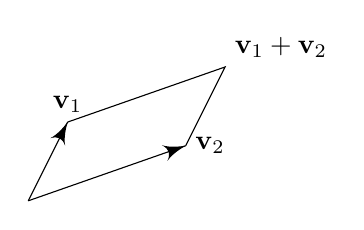
\begin{tikzpicture}
      \draw [->] (0, 0) -- (.5, 1) node [above] {$\mathbf{v}_1$};
      \draw [->] (0, 0) -- (2, .7) node [right] {$\mathbf{v}_2$};
      \draw (.5, 1) -- (2.5, 1.7) node [anchor=south west] {$\mathbf{v}_1 + \mathbf{v}_2$} -- (2, .7);
    \end{tikzpicture}
  \end{center}
  Then a closed disc $S$ around $0$ contains a non-zero point of $\Lambda$ if
  \[
    \area(S) \geq 4 A(\Lambda).
  \]
  In particular, there exists an $\alpha \in \Lambda$ with $\alpha \not= 0$, such that
  \[
    0 < |\alpha|^2 \leq \frac{4 A(\Lambda)}{\pi}.
  \]
\end{lemma}
This is just an easy piece of geometry. What is remarkable is that the radius of the disc needed depends only on the area of the fundamental parallelogram, and not its shape.

\begin{proof}
  We will prove a general result in any dimensions later.
\end{proof}

We now apply this to ideals $\mathfrak{a} \leq \mathcal{O}_L$, regarded as a subset of $\C = \R^2$ via some embedding $L \hookrightarrow \C$. The following proposition gives us the areas of the relevant lattices:

\begin{prop}\leavevmode
  \begin{enumerate}
    \item If $\alpha = a + b\sqrt{\lambda}$, then as a complex number,
      \[
        |\alpha|^2 = (a + b\sqrt{\lambda})(a - b\sqrt{\lambda}) = N(\alpha).
      \]
    \item For $\mathcal{O}_L$, we have
      \[
        A(\mathcal{O}_L) = \frac{1}{2}\sqrt{|D_L|}.
      \]
    \item In general, we have
      \[
        A(\mathfrak{a}) = \frac{1}{2} \sqrt{|\Delta(\alpha_1, \alpha_2)|},
      \]
      where $\alpha_1, \alpha_2$ are the integral basis of $\mathfrak{a}$.
    \item We have
      \[
        A(\mathfrak{a}) = N(\mathfrak{a}) A(\mathcal{O}_L).
      \]
  \end{enumerate}
\end{prop}

\begin{proof}\leavevmode
  \begin{enumerate}
    \item This is clear.
    \item We know $\mathcal{O}_L$ has basis $1, \alpha$, where again
      \[
        \alpha =
        \begin{cases}
          \sqrt{d} & d \equiv 2, 3\pmod 4\\
          \frac{1}{2}(1 + \sqrt{d})& d \equiv 1 \pmod 4
        \end{cases}.
      \]
      So we can just look at the picture of the lattice, and compute to get
      \[
        A(\mathcal{O}_L) =
        \begin{cases}
          \sqrt{|d|} & d \equiv 2, 3 \pmod 4\\
          \frac{1}{2}\sqrt{|d|} & d \equiv 1\pmod 4
        \end{cases} = \frac{1}{2}\sqrt{|D_L|}.
      \]
    \item If $\alpha_1, \alpha_2$ are the integral basis of $\mathfrak{a}$, then the lattice of $\mathfrak{a}$ is in fact spanned by the vectors $\alpha_1 = a + bi, \alpha_2 = a' + b' i$. This has area
      \[
        A(\mathfrak{a}) = \det
        \begin{pmatrix}
          a & b\\
          a' & b'
        \end{pmatrix},
      \]
      whereas we have
      \begin{align*}
        \Delta(\alpha_1, \alpha_2) &=
        \det
        \begin{pmatrix}
          \alpha_1 & \bar{\alpha}_1\\
          \alpha_2 & \bar{\alpha}_2
        \end{pmatrix}^2\\
        &= (\alpha_1 \bar{\alpha}_2 - \alpha_2 \bar{\alpha}_1)^2\\
        &= \Im(2\alpha_1 \bar{\alpha}_2)^2\\
        &= 4(a'b - ab')^2\\
        &= 4A(\mathfrak{a})^2.
      \end{align*}
    \item This follows from (ii) and (iii), as
      \[
        \Delta(\alpha_1, \cdots, \alpha_n) = N(\mathfrak{a})^2 D_L
      \]
      in general.
  \end{enumerate}
\end{proof}

Now what does Minkowski's lemma tell us? We know there is an $\alpha \in \mathfrak{a}$ such that
\[
  N(\alpha) \leq \frac{4A(\mathfrak{a})}{\pi} = N(\mathfrak{a}) c_L,
\]
where
\[
  c_L = \frac{2\sqrt{|D_L|}}{\pi}.
\]
But $\alpha \in \mathfrak{a}$ implies $\bra \alpha\ket \subseteq \mathfrak{a}$, which implies $\bra \alpha\ket = \mathfrak{a} \mathfrak{b}$ for some ideal $\mathfrak{b}$. So
\[
  |N(\alpha)| = N(\bra \alpha\ket) = N(\mathfrak{a})N(\mathfrak{b}).
\]
So this implies
\[
  N(\mathfrak{b}) \leq c_L = \frac{2\sqrt{|D_L|}}{\pi}.
\]
Recall that the class group is $\cl_L = I_L/P_L$, the fractional ideals quotiented by principal ideals, and we write $[\mathfrak{a}]$ for the class of $\mathfrak{a}$ in $\cl_L$. Then if $\mathfrak{a}\mathfrak{b} = \bra \alpha\ket$, then we have
\[
  [\mathfrak{b}] = [\mathfrak{a}^{-1}]
\]
in $\cl_L$. So we have just shown,
\begin{prop}[Minkowski bound]\index{Minkowski bound}
  For all $[\mathfrak{a}] \in \cl_L$, there is a representative $\mathfrak{b}$ of $[\mathfrak{a}]$ (i.e.\ an ideal $\mathfrak{b} \leq \mathcal{O}_L$ such that $[\mathfrak{b}] = [\mathfrak{a}]$) such that
  \[
    N(\mathfrak{b}) \leq c_L = \frac{2\sqrt{|D_L|}}{\pi}.
  \]
\end{prop}

\begin{proof}
  Find the $\mathfrak{b}$ such that $[\mathfrak{b}] = [(\mathfrak{a}^{-1})^{-1}]$ and $N(\mathfrak{b}) \leq c_L$.
\end{proof}

Combining this with the following easy lemma, we know that the class group is finite!
\begin{lemma}
  For every $n \in \Z$, there are only finitely many ideals $\mathfrak{a} \leq \mathcal{O}_L$ with $N(\mathfrak{a}) = m$.
\end{lemma}

\begin{proof}
  If $N(\mathfrak{a}) = m$, then by definition $|\mathcal{O}_L/\mathfrak{a}| = m$. So $m \in \mathfrak{a}$ by Lagrange's theorem. So $\bra m \ket \subseteq \mathfrak{a}$, i.e.\ $\mathfrak{a} \mid \bra m\ket$. Hence $\mathfrak{a}$ is a factor of $\bra m\ket$. By unique factorization of prime ideals, there are only finitely many such ideals.
\end{proof}

Another proof is as follows:
\begin{proof}
  Each ideal bijects with an ideal in $\mathcal{O}_L/m\mathcal{O}_L = (\Z/m)^n$. So there are only finitely many.
\end{proof}

Thus, we have proved
\begin{thm}
  The class group $\cl_L$ is a finite group, and the divisors of ideals of the form $\bra p\ket$ for $p \in \Z$, $p$ a prime, and $0 < p < c_L$, collectively generate $\cl_L$.
\end{thm}

\begin{proof}\leavevmode
  \begin{enumerate}
    \item Each element is represented by an ideal of norm less than $2\sqrt{|D_L|}/\pi$, and there are only finitely many ideals of each norm.
    \item Given any element of $\cl_L$, we pick a representative $\mathfrak{a}$ such that $N(\mathfrak{a}) < c_L$. We factorize
      \[
        \mathfrak{a}= \mathfrak{p}_1^{e_1} \cdots \mathfrak{p}_r^{e_r}.
      \]
      Then
      \[
        N(\mathfrak{p}_i) \leq N(\mathfrak{a}) < c_L.
      \]
      Suppose $\mathfrak{p}_i \mid \bra p\ket$. Then $N(\mathfrak{p})$ is a power of $p$, and is thus at least $p$. So $p < c_L$.
  \end{enumerate}
\end{proof}

We now try to work with some explicit examples, utilizing Dedekind's criterion and the Minkowski bound.
\begin{eg}
  Consider $d = -7$. So $\Q(\sqrt{-7}) = L$, and $D_L = -7$. Then we have
  \[
    1 < c_L = \frac{2\sqrt{7}}{\pi} < 2.
  \]
  So $\cl_L = \{1\}$, since there are no primes $p < c_L$. So $\mathcal{O}_L$ is a UFD.

  Similarly, if $d = -1, -2, -3$, then $\mathcal{O}_L$ is a UFD.
\end{eg}

\begin{eg}
  Let $d = -5$. Then $D_L = -20$. We have
  \[
    2 < c_L = \frac{4\sqrt{5}}{\pi} < 3.
  \]
  So $\cl_L$ is generated by primes dividing $\bra 2\ket$.

  Recall that Dirichlet's theorem implies
  \[
    \bra 2\ket = \bra 2, 1 + \sqrt{-5}\ket^2 = \mathfrak{p}^2.
  \]
  Also, $\mathfrak{p} = \bra 2, 1 + \sqrt{-5}\ket$ is not principal. If it were, then $\mathfrak{p} = \bra \beta\ket$, with $\beta = x + y \sqrt{-5}$, and $N(\beta) = 2$. But there are no solutions in $\Z$ of $x^2 + 5y^2 = 2$. So $\cl_L = \bra \mathfrak{p}\ket = \Z/2$.
\end{eg}

\begin{eg}
  Consider $d = -17 \equiv 3 \pmod 4$. So $c_L \sim 5.3$. So $\cl_L$ is generated by primes dividing by $\bra 2\ket, \bra 3\ket, \bra 5\ket$. We factor
  \[
    x^2 + 17 \equiv x^2 + 1 \equiv (x + 1)^2 \pmod 2.
  \]
  So
  \[
    \bra 2\ket = \mathfrak{p}^2 = \bra 2, 1 + \sqrt{d}\ket^2.
  \]
  Doing this mod $3$, we have
  \[
    x^2 + 17 \equiv x^2 - 1 \equiv (x - 1)(x + 1) \pmod 3.
  \]
  So we have
  \[
    \bra 3\ket = \mathfrak{q}\bar{\mathfrak{q}} = \bra 3, 1 + \sqrt{d}\ket \bra 3, 1 - \sqrt{d}\ket.
  \]
  Finally, mod $5$, we have
  \[
    x^2 + 17 \equiv x^2 + 2 \pmod 5.
  \]
  So $5$ is inert, and $[\bra 5\ket] = 1$ in $\cl_L$. So
  \[
    \cl_L = \bra [\mathfrak{p}], [\mathfrak{q}]\ket,
  \]
  and we need to compute what this is. We can just compute powers $\mathfrak{q}^2, \mathfrak{q}^3, \cdots$, $\mathfrak{p}\mathfrak{q}, \mathfrak{p}\mathfrak{q}^2, \cdots$, and see what happens.

  But a faster way is to look for principal ideals with small norms that are multiples of $2$ and $3$. For example,
  \[
    N(\bra 1 + \sqrt{d}\ket) = 18 = 2 \cdot 3^2.
  \]
  But we have
  \[
    1 + \sqrt{d} \in \mathfrak{p}, \mathfrak{q}.
  \]
  So $\mathfrak{p}, \mathfrak{q} \mid \bra 1 + \sqrt{d}\ket$. Thus we know $\mathfrak{p}\mathfrak{q} \mid \bra 1 + \sqrt{d}\ket$. We have $N(\mathfrak{p}\mathfrak{q}) = 2 \cdot 3 = 6$. So there is another factor of $3$ to account for. In fact, we have
  \[
    \bra 1 + \sqrt{d}\ket = \mathfrak{p}\mathfrak{q}^2,
  \]
  which we can show by either thinking hard or expanding it out. So we must have
  \[
    [\mathfrak{p}] = [\mathfrak{q}]^{-2}
  \]
  in $\cl_L$. So we have $\cl_L = \bra [\mathfrak{q}]\ket$. Also, $[\mathfrak{q}]^{-2} = [\mathfrak{p}] \not= 1$ in $\cl_L$, as if it did, then $\mathfrak{p}$ is principal, i.e.\ $\mathfrak{p} = \bra x + y\sqrt{d}\ket$, but $2 = N(\mathfrak{p}) = x^2 + 7y^2$ has no solution in the integers. Also, we know $[\mathfrak{p}]^2 = [1]$. So we know
  \[
    \cl_L = \Z/4\Z.
  \]
\end{eg}

In fact, we have
\begin{thm}
  Let $L = \Q(\sqrt{d})$ with $d < 0$. Then $\mathcal{O}_L$ is a UFD if
  \[
    -d \in \{1, 2, 3, 7, 11, 19, 43, 67, 163\}.
  \]
  Moreover, this is actually an ``if and only if''.
\end{thm}
The first part is a straightforward generalization of what we have been doing, but the proof that no other $d$'s work is \emph{hard}.

\subsection*{General case}
Now we want to extend these ideas to higher dimensions. We are really just doing the same thing, but we need a bit harder geometry and proper definitions.

\begin{defi}[Discrete subset]\index{discrete subset}
  A subset $X \subseteq \R^n$ is \emph{discrete} if for every $x \in X$, there is some $\varepsilon > 0$ such that $B_\varepsilon(x) \cap X = \{x\}$. This is true if and only if for every compact $K \subseteq \R^n$, $K\cap X$ is finite.
\end{defi}

We have the following very useful characterization of discrete subgroups of $\R^n$:
\begin{prop}
  Suppose $\Lambda \subseteq \R^n$ is a subgroup. Then $\Lambda$ is a discrete subgroup of $(\R^n, +)$ if and only if
  \[
    \Lambda = \left\{\sum_1^m n_i \mathbf{x}_i : n_i \in \Z\right\}
  \]
  for some $\mathbf{x}_1, \cdots, \mathbf{x}_n$ linearly independent over $\R$.
\end{prop}

Note that linear independence is important. For example, $\Z \sqrt{2} + \Z \sqrt{3} \subseteq \R$ is not discrete. On the other hand, if $\Lambda = \mathfrak{a} \lhd \mathcal{O}_L$ is an ideal, where $L = \Q(\sqrt{d})$ and $d < 0$, then this is discrete.

\begin{proof}
  Suppose $\Lambda$ is generated by $\mathbf{x}_1, \cdots, \mathbf{x}_m$. By linear independence, there is some $g \in \GL_n(\R)$ such that $g \mathbf{x}_i = \mathbf{e}_i$ for all $1 \leq i \leq m$, where $\mathbf{e}_1, \cdots, \mathbf{e}_n$ is the standard basis. We know acting by $g$ preserves discreteness, since it is a homeomorphism, and $g\Lambda = \Z^m \subseteq \R^m \times \R^{n - m}$ is clearly discrete (take $\varepsilon = \frac{1}{2}$). So this direction follows.

  For the other direction, suppose $\Lambda$ is discrete. We pick $\mathbf{y}_1, \cdots, \mathbf{y}_m \in \Lambda$ which are linearly independent over $\R$, with $m$ maximal (so $m \leq n$). Then by maximality, we know
  \[
    \left\{\sum_{i = 1}^m \lambda_i \mathbf{y}_i: \lambda_i \in \R\right\} = \left\{ \sum_1^m \lambda_i \mathbf{z}_i: \lambda_i \in \R, \mathbf{z}_i \in \Lambda\right\},
  \]
  and this is the smallest vector subspace of $\R^n$ containing $\Lambda$. We now let
  \[
    X = \left\{\sum_{i = 1}^m \lambda_i \mathbf{y}_i: \lambda_i \in [0, 1]\right\} \cong [0, 1]^m.
  \]
  This is closed and bounded, and hence compact. So $X \cap \Lambda$ is finite.

  Also, we know
  \[
    \bigoplus \Z \mathbf{y}_i = \Z^m \subseteq \Lambda,
  \]
  and if $\gamma$ is any element of $\Lambda$, we can write it as $\gamma = \gamma_0 + \gamma_1$, where $\gamma_0 \in X$ and $\gamma_1 \in \Z^m$. So
  \[
    \left|\frac{\Lambda}{\Z^m}\right| \leq |X \cap \Lambda| < \infty.
  \]
  So let $d = |\Lambda/\Z^m|$. Then $d \Lambda \subseteq \Z^m$, i.e.\ $\Lambda \subseteq \frac{1}{d} \Z^m$. So
  \[
    \Z^m \subseteq \Lambda \subseteq \frac{1}{d} \Z^m.
  \]
  So $\Lambda$ is a free abelian group of rank $m$. So there exists $\mathbf{x}_1, \cdots, \mathbf{x}_m \in \frac{1}{d}\Z^m$ which is an integral basis of $\Lambda$ and are linearly independent over $\R$.
\end{proof}

\begin{defi}[Lattice]\index{lattice}
  If $\rank \Lambda = n = \dim \R^n$, then $\Lambda$ is a \emph{lattice} in $\R^n$.
\end{defi}

\begin{defi}[Covolume and fundamental domain]\index{covolume}\index{fundamental domain}
  Let $\Lambda \subseteq \R^n$ be a lattice, and $\mathbf{x}_1, \cdots, \mathbf{x}_n$ be a basis of $\Lambda$, then let
  \[
    P = \left\{\sum_{i = 1}^n \lambda_i \mathbf{x}_i: \lambda_i \in [0, 1]\right\},
  \]
  and define the \emph{covolume} of $\Lambda$ to be
  \[
    \covol(\Lambda) = \vol(P) = |\det A|,
  \]
  where $A$ is the matrix such that $\mathbf{x}_i = \sum a_{ij} \mathbf{e}_j$.

  We say $P$ is a \emph{fundamental domain} for the action of $\Lambda$ on $\R^n$, i.e.
  \[
    \R^n = \bigcup_{\gamma \in \Lambda} (\gamma + P),
  \]
  and
  \[
    (\gamma + P) \cap (\mu + P) \subseteq \partial (\gamma + P).
  \]
  In particular, the intersection has zero volume.
\end{defi}
This is called the covolume since if we consider the space $\R^n/ \Lambda$, which is an $n$-dimensional torus, then this has volume $\covol (\Lambda)$.

Observe now that if $\mathbf{x}_1', \cdots, \mathbf{x}_n'$ is a different basis of $\Lambda$, then the transition matrix $\mathbf{x}_i' = \sum b_{ij} \mathbf{x}_j$ has $B \in \GL_n (\Z)$. So we have $\det B = \pm 1$, and $\covol (\Lambda)$ is independent of the basis choice.

With these notations, we can now state Minkowski's theorem.

\begin{thm}[Minkowski's theorem]\index{Minkowski's theorem}
  Let $\Lambda \subseteq \R^n$ be a lattice, and $P$ be a fundamental domain. We let $S \subseteq \R^n$ be a measurable set, i.e.\ one for which $\vol(S)$ is defined.
  \begin{enumerate}
    \item Suppose $\vol(S) > \covol(\Lambda)$. Then there exists distinct $\mathbf{x}, \mathbf{y} \in S$ such that $\mathbf{x} - \mathbf{y} \in \Lambda$.
    \item Suppose $\mathbf{0} \in S$, and $S$ is symmetric around $0$, i.e.\ $\mathbf{s} \in S$ if and only if $-\mathbf{s} \in S$, and $S$ is convex, i.e.\ for all $\mathbf{x}, \mathbf{y} \in S$ and $\lambda \in [0, 1]$, then
      \[
        \lambda \mathbf{x} + (1 - \lambda)\mathbf{y} \in S.
      \]
      Then suppose either
      \begin{enumerate}
        \item $\vol (S) > 2^n \covol(\Lambda)$; or
        \item $\vol (S) \geq 2^n \covol(\Lambda)$ and $S$ is closed.
      \end{enumerate}
      Then $S$ contains a $\gamma \in \Lambda$ with $\gamma \not= 0$.
  \end{enumerate}
\end{thm}

Note that for $n = 2$, this is what we used for quadratic fields.

By considering $\Lambda = \Z^n \subseteq \R^n$ and $S = [-1, 1]^n$, we know the bounds are sharp.

\begin{proof}\leavevmode
  \begin{enumerate}
    \item Suppose $\vol(S) > \covol(\Lambda) = \vol(P)$. Since $P \subseteq \R^n$ is a fundamental domain, we have
      \[
        \vol(S) = \vol(S \cap \R^n) = \vol\left(S \cap \sum_{\gamma \in \Lambda} (P + \gamma)\right) = \sum_{\gamma \in \Lambda} \vol(S \cap (P + \gamma)).
      \]
      Also, we know
      \[
        \vol(S \cap (P + \gamma)) = \vol((S - \gamma) \cap P),
      \]
      as volume is translation invariant. We now claim the sets $(S - \gamma) \cap P$ for $\gamma \in \Lambda$ are \emph{not} pairwise disjoint. If they were, then
      \[
        \vol(P) \geq \sum_{\gamma \in \Lambda} \vol((S - \gamma) \cap P) = \sum_{\gamma \in \Lambda} \vol(S \cap (P + \gamma)) = \vol(S),
      \]
      contradicting our assumption.

      Then in particular, there are some distinct $\gamma$ and $\mu$ such that $(S - \gamma)$ and $(S - \mu)$ are not disjoint. In other words, there are $\mathbf{x}, \mathbf{y} \in S$ such that $\mathbf{x} - \gamma = \mathbf{y} - \mu$, i.e.\ $\mathbf{x} - \mathbf{y} = \gamma - \mu \in \Lambda \not= 0$.
    \item We now let
      \[
        S' = \frac{1}{2} S = \left\{\frac{1}{2}s: s \in S\right\}.
      \]
      So we have
      \[
        \vol(S') = 2^{-n} \vol(S) > \covol(\Lambda),
      \]
      by assumption.
      \begin{enumerate}
        \item So there exists some distinct $\mathbf{y}, \mathbf{z} \in S'$ such that $\mathbf{y} - \mathbf{z} \in \Lambda \setminus \{0\}$. We now write
          \[
            \mathbf{y} - \mathbf{z} = \frac{1}{2} (2\mathbf{y} + (-2\mathbf{z})),
          \]
          Since $2\mathbf{z} \in S$ implies $-2\mathbf{z} \in S$ by symmetry around $\mathbf{0}$, so we know $\mathbf{y} - \mathbf{z} \in S$ by convexity.
        \item We apply the previous part to $S_m = \left(1 + \frac{1}{m}\right)S$ for all $m \in \N$, $m > 0$. So we get a non-zero $\gamma_m \in S_m \cap \Lambda$.

          By convexity, we know $S_m \subseteq S_1 = 2S$ for all $m$. So $\gamma_1, \gamma_2, \cdots \in S_1 \cap \Lambda$. But $S_1$ is compact set. So $S_1 \cap \Lambda$ is finite. So there exists $\gamma$ such that $\gamma_m$ is $\gamma$ infinitely often. So
          \[
            \gamma \in \bigcap_{m \geq 0} S_m = S.
          \]
          So $\gamma \in S$.
      \end{enumerate}
  \end{enumerate}
\end{proof}

We are now going to use this to mimic our previous proof that the class group of an imaginary quadratic field is finite.

To begin with, we need to produce lattices from ideals of $\mathcal{O}_L$. Let $L$ be a number field, and $[L:\Q] = n$. We let $\sigma_1, \cdots,\sigma_r: L \to \R$ be the real embeddings, and $\sigma_{r + 1}, \cdots, \sigma_{r + s},\bar{\sigma}_{r + 1}, \cdots, \bar{\sigma}_{r + s}: L \to \C$ be the complex embeddings (note that which embedding is $\sigma_{r + i}$ and which is $\bar{\sigma}_{r + i}$ is an arbitrary choice).

Then this defines an embedding
\[
  \sigma = (\sigma_1, \sigma_2, \cdots, \sigma_r, \sigma_{r + 1}, \cdots, \sigma_{r + s}): L \hookrightarrow \R^r \times \C^s \cong \R^r \times \R^{2s} = \R^{r + 2s} = \R^n,
\]
under the isomorphism $\C \to \R^2$ by $x + iy \mapsto (x, y)$.

Just as we did for quadratic fields, we can relate the norm of ideals to their covolume.

\begin{lemma}\leavevmode
  \begin{enumerate}
    \item $\sigma(\mathcal{O}_L)$ is a lattice in $\R^n$ of covolume $2^{-s} |D_L|^{\frac{1}{2}}$.
    \item More generally, if $\mathfrak{a} \lhd \mathcal{O}_L$ is an ideal, then $\sigma(\mathfrak{a})$ is a lattice and the covolume
      \[
        \covol(\sigma(\mathfrak{a})) = 2^{-s} |D_L|^{\frac{1}{2}} N(\mathfrak{a}).
      \]
  \end{enumerate}
\end{lemma}

\begin{proof}
  Obviously (ii) implies (i). So we just prove (ii). Recall that $\mathfrak{a}$ has an integral basis $\gamma_1, \cdots, \gamma_n$. Then $\mathfrak{a}$ is the integer span of the vectors
  \[
    (\sigma_1(\gamma_i), \sigma_2(\gamma_i), \cdots, \sigma_{r + s}(\gamma_i))
  \]
  for $i = 1, \cdots, n$, and they are independent as we will soon see when we compute the determinant. So it is a lattice.

  We also know that
  \[
    \Delta(\gamma_1, \cdots, \gamma_n) = \det (\sigma_i(\gamma_j))^2 = N(\mathfrak{a})^2 D_L,
  \]
  where the $\sigma_i$ run over all $\sigma_1, \cdots, \sigma_r, \sigma_{r + 1}, \cdots, \sigma_{r + s}, \bar{\sigma}_{r + 1}, \cdots \bar{\sigma}_{r + s}$.

  So we know
  \[
    |\det (\sigma_i(\gamma_j))| = N(\mathfrak{a}) |D_L|^{\frac{1}{2}}.
  \]
  So what we have to do is to relate $\det(\sigma_i(\gamma_j))$ to the covolume of $\sigma(\mathfrak{a})$. But these two expressions are very similar.

  In the $\sigma_i (\gamma_j)$ matrix, we have columns that look like
  \[
    \begin{pmatrix}
      \sigma_{r + i}(\gamma_j) & \bar{\sigma}_{r + i}(\gamma_j)
    \end{pmatrix} =
    \begin{pmatrix}
      z & \bar{z}
    \end{pmatrix}.
  \]
  On the other hand, the matrix of $\sigma(\gamma)$ has corresponding entries
  \[
    \begin{pmatrix}
      \Re(z) & \Im(z)
    \end{pmatrix} =
    \begin{pmatrix}
      \frac{1}{2}(z + \bar{z}) &\frac{i}{2}(\bar{z} - z)
    \end{pmatrix} =
    \frac{1}{2}
    \begin{pmatrix}
      1 & 1\\
      i & -i
    \end{pmatrix}
    \begin{pmatrix}
      z\\\bar{z}
    \end{pmatrix}
  \]
  We call the last matrix $A = \displaystyle\frac{1}{2}\begin{pmatrix}1 & 1\\i & -i\end{pmatrix}$. We can compute the determinant as
  \[
    |\det A| = \left|\det \frac{1}{2}
    \begin{pmatrix}
      1 & 1\\
      i & -i
    \end{pmatrix}\right| = \frac{1}{2}.
  \]
  Hence the change of basis matrix from $(\sigma_i(\gamma_j))$ to $\sigma(\gamma)$ is $s$ diagonal copies of $A$, so has determinant $2^{-s}$. So this proves the lemma.
\end{proof}

\begin{prop}
  Let $\mathfrak{a} \lhd \mathcal{O}_L$ be an ideal. Then there exists an $\alpha \in \mathfrak{a}$ with $\alpha \not= 0$ such that
  \[
    |N(\alpha)| \leq c_L N(\mathfrak{a}),
  \]
  where
  \[
    c_L = \left(\frac{4}{\pi}\right)^s \frac{n!}{n^n} |D_L|^{\frac{1}{2}}.
  \]\qedhere
\end{prop}
This is the \emph{Minkowski bound}\index{Minkowski bound}.

\begin{proof}
  Let
  \[
    B_{r, s}(t) = \left\{(y_1, \cdots, y_r, z_1, \cdots, z_s) \in \R^r \times \C^s: \sum |y_i| + 2 \sum |z_i| \leq t\right\}.
  \]
  This
  \begin{enumerate}
    \item is closed and bounded;
    \item is measurable (it is defined by polynomial inequalities);
    \item has volume
      \[
        \vol(B_{r, s}(t)) = 2^r \left(\frac{\pi}{2}\right)^s \frac{t^n}{n!};
      \]
    \item is convex and symmetric about $0$.
  \end{enumerate}
  Only (iii) requires proof, and it is on the second example sheet, i.e.\ we are not doing it here. It is just doing the integral.

  We now choose $t$ so that
  \[
    \vol B_{r, s}(t) = 2^n \covol(\sigma(\mathfrak{a})).
  \]
  Explicitly, we let
  \[
    t^n = \left(\frac{4}{\pi}\right)^s n! |D_L|^{1/2}N(\mathfrak{a}).
  \]
  Then by Minkowski's lemma, there is some $\alpha \in \mathfrak{a}$ non-zero such that $\sigma(\alpha) \in B_{r, s}(t)$. We write
  \[
    \sigma(\alpha) = (y_1, \cdots, y_r, z_1, \cdots, z_s).
  \]
  Then we observe
  \[
    N(\alpha) = y_1\cdots y_r z_1 \bar{z}_1 z_2 \bar{z}_2 \cdots z_s \bar{z}_s = \prod y_i \prod|z_j|^2.
  \]
  By the AM-GM inequality, we know
  \[
    |N(\alpha)|^{1/n} \leq \frac{1}{n}\left(\sum y_i + 2 \sum |z_j|\right) \leq \frac{t}{n},
  \]
  as we know $\sigma(\mathfrak{a}) \in B_{r, s}(t)$. So we get
  \[
    |N(\alpha)| \leq \frac{t^n}{n^n} = c_L N(\mathfrak{a}).
  \]
\end{proof}

\begin{cor}
  Every $[\mathfrak{a}] \in \cl_L$ has a representative $\mathfrak{a} \in \mathcal{O}_L$ with $N(\mathfrak{a}) \leq c_L$.
\end{cor}

\begin{thm}[Dirichlet]\index{finiteness of class group}\index{class group!finiteness}
  The class group $\cl_L$ is finite, and is generated by prime ideals of norm $\leq c_L$.
\end{thm}

\begin{proof}
  Just as the case for imaginary quadratic fields.
\end{proof}

\section{Dirichlet's unit theorem}
We have previously characterized the units on $\mathcal{O}_L$ as the elements with unit norm, i.e.\ $\alpha \in \mathcal{O}_L$ is a unit if and only if $|N(\alpha)| = 1$. However, this doesn't tell us much about how many units there are, and how they are distributed. The answer to this question is given by Dirichlet's unit theorem.

\begin{thm}[Dirichlet unit theorem]\index{Dirichlet unit theorem}
  We have the isomorphism
  \[
    \mathcal{O}_L^\times \cong \mu_L \times \Z^{r + s - 1},
  \]
  where
  \[
    \mu_L = \{\alpha \in L: \alpha^N = 1\text{ for some }N > 0\}
  \]
  is the group of roots of unity in $L$, and is a finite cyclic group.
\end{thm}

Just as in the finiteness of the class group, we do it for an example first, or else it will be utterly incomprehensible.

We do the example of \emph{real} quadratic fields, $L = \Q[\sqrt{d}]$, where $d > 1$ is square-free. So $r = 2, s = 0$, and $L \subseteq \R$ implies $\mu_L = \{\pm 1\}$. So
\[
  \mathcal{O}_L^\times \cong \{\pm 1\} \times \Z.
\]
Also, we know that
\[
  N(x + y\sqrt{d}) = (x + y\sqrt{d})(x - y\sqrt{d}) = x^2 - dy^2.
\]
So Dirichlet's theorem is saying that there are infinitely many solutions of $x^2 - dy^2 = \pm 1$, and are all (plus or minus) the powers of one single element.

\begin{thm}[Pell's equation]\index{Pell's equation}
  There are infinitely many $x + y\sqrt{d} \in \mathcal{O}_L$ such that $x^2 - dy^2 = \pm 1$.
\end{thm}
You might have seen this in IIC Number Theory, where we proved it directly by continued fractions. We will provide a totally unconstructive proof here, since this is more easily generalized to arbitrary number fields.

This is actually just half of Dirichlet's theorem. The remaining part is to show that they are all powers of the same element.
\begin{proof}
  Recall that $\sigma: \mathcal{O}_L \to \R^2$ sends
  \[
    \alpha = x + y\sqrt{d} \mapsto (\sigma_1(\alpha), \sigma_2(\alpha)) = (x + y\sqrt{d}, x - y\sqrt{d}).
  \]
  (in the domain, $\sqrt{d}$ is a formal symbol, while in the codomain, it is a real number, namely the positive square root of $d$)

  Also, we know
  \[
    \covol(\sigma(\mathcal{O}_L)) = |D_L|^{\frac{1}{2}}.
  \]
  \begin{center}
    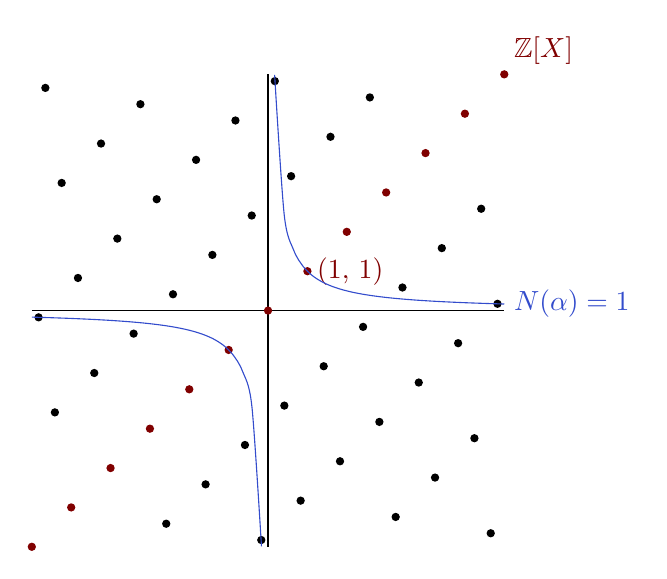
\begin{tikzpicture}[scale=0.5]
      \draw (-6, 0) -- (6, 0);
      \draw (0, -6) -- (0, 6);
      \foreach \x in {-6,...,6} {
        \node [mred, circ] at (\x, \x) {};
      }
      \foreach \y/\n in {1/4,2/3, 3/1, 4/0} {
        \foreach \x in {-\n,...,\n} {
          \node [circ] at (\x + \y *1.414, \x - \y *1.414) {};
        }
        \foreach \x in {-\n,...,\n} {
          \node [circ] at (\x - \y *1.414, \x + \y *1.414) {};
        }
      }

      \node [mred, right] at (1, 1) {(1, 1)};
      \node [mred, anchor = south west] at (6, 6) {$\Z[X]$};

      \draw [mblue, domain=0.167:6] plot [smooth] (\x, {1/\x});
      \draw [mblue, domain=0.167:6] plot [smooth] ({-\x}, {-1/\x});

      \node [mblue, right] at (6, 0.167) {$N(\alpha) = 1$};
    \end{tikzpicture}
  \end{center}
  Consider
  \[
    s_t = \left\{(y_1, y_2) \in \R^2: |y_1|\leq t, |y_2| \leq \frac{|D_L|^{1/2}}{t}\right\}.
  \]
  So
  \[
    \vol(s_t) = 4|D_L|^{\frac{1}{2}} = 2^n \covol(\mathcal{O}_L),
  \]
  as $n = [L:\Q] = 2$. Now Minkowski implies there is an $\alpha \in \mathcal{O}_L$ non-zero such that $\sigma(\alpha) \in s_t$. Also, if we write
  \[
    \sigma(\alpha) = (y_1, y_2),
  \]
  then
  \[
    N(\alpha) = y_1y_2.
  \]
  So such an $\alpha$ will satisfy
  \[
    1 \leq |N(\alpha)| \leq |D_L|^{1/2}.
  \]
  This is not quite what we want, since we need $|N(\alpha)| = 1$ exactly. Nevertheless, this is a good start. So let's try to find infinitely such elements.

  First notice that no points on the lattice (apart from the origin) hits the $x$ or $y$ axis, since any such point must satisfy $x \pm y\sqrt{d} = 0$, but $\sqrt{d}$ is not rational. Also, $s_t$ is compact. So $s_t \cap \sigma(\mathcal{O}_L)$ contains finitely many points. So we can find a $t_2$ such that for each $(y_1, y_2) \in s_t \cap \mathcal{O}_L$, we have $|y_1| > t_2$. In particular, $s_{t_2}$ does not contain any point in $s_t \cap \sigma(\mathcal{O}_L)$. So we get a new set of points $\alpha \in s_{t_2} \cap \mathcal{O}_L$ such that $1 \leq |N(\alpha)| \leq |D_L|^{1/2}$.
  \begin{center}
    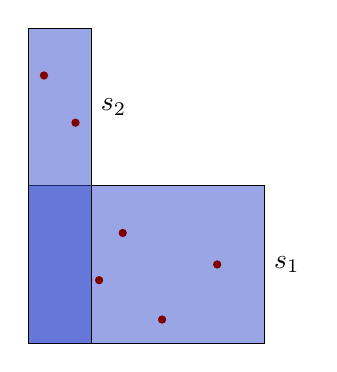
\begin{tikzpicture}
      \draw [fill=mblue, fill opacity=0.5] (0, 0) rectangle (3, 2);
      \node at (3, 1) [right] {$s_1$};

      \node [circ, mred] at (0.9, 0.8) {};
      \node [circ, mred] at (1.7, 0.3) {};
      \node [circ, mred] at (1.2, 1.4) {};
      \node [circ, mred] at (2.4, 1.0) {};

      \draw [fill=mblue, fill opacity=0.5] (0, 0) rectangle (0.8, 4);
      \node at (0.8, 3) [right] {$s_2$};

      \node [circ, mred] at (0.2, 3.4) {};
      \node [circ, mred] at (0.6, 2.8) {};
    \end{tikzpicture}
  \end{center}
  We can do the same thing for $s_{t_2}$ and get a new $t_3$. In general, given $t_1 > \cdots > t_n$, pick $t_{n + 1}$ be such that
  \[
    0 < t_{n + 1} < \min\left\{|y_1|: (y_1, y_2) \in \bigcup_{i = 1}^n s_{t_i} \cap \sigma(\mathcal{O}_L)\right\},
  \]
  and the minimum is finite since $s_t$ is compact and hence contains finitely many lattice points on $\sigma(\mathcal{O}_L)$.

  Then we get an infinite sequence of $t_i$ such that $s_{t_i} \cap \sigma(\mathcal{O}_L)$ are disjoint for different $i$. Since each must contain at least one point, we have got infinitely many points in $\mathcal{O}_L$ satisfying $1 \leq |N(\alpha)| \leq |D_L|^{1/2}$.

  Since there are only finitely many integers between $1$ and $|D_L|^{1/2}$, we can apply the pigeonhole principle, and get that there is some integer satisfying $1 \leq |m| \leq |D_L|^{1/2}$ such that there exists infinitely many $\alpha \in \mathcal{O}_L$ with $N(\alpha) = m$.

  This is not quite good enough. We consider
  \[
    \mathcal{O}_L/m\mathcal{O}_L \cong (\Z/m\Z)^{[L:\Q]},
  \]
  another finite set. We notice that each $\alpha \in \mathcal{O}_L$ must fall into one of finitely many the cosets of $m\mathcal{O}_L$ in $\mathcal{O}_L$. In particular, each $\alpha$ such that $N(\alpha) = m$ must belong to one of these cosets.

  So again by the pigeonhole principle, there exists a $\beta \in \mathcal{O}_L$ with $N(\beta) = m$, and infinitely many $\alpha \in \mathcal{O}_L$ with $N(\alpha) = m$ and $\alpha = \beta \pmod {m\mathcal{O}_L}$.

  Now of course $\alpha$ and $\beta$ are not necessarily units, if $m \not= 1$. However, we will show that $\alpha/\beta$ is. The hard part is of course showing that it is in $\mathcal{O}_L$ itself, because it is clear that $\alpha/\beta$ has norm $1$ (alternatively, by symmetry, $\beta/\alpha$ is in $\mathcal{O}_L$, so an inverse exists).

  Hence all it remains is to prove the general fact that if
  \[
    \alpha = \beta + m\gamma,
  \]
  where $\alpha, \beta, \gamma \in \mathcal{O}_L$ and $N(\alpha) = N(\beta) = m$, then $\alpha/\beta \in \mathcal{O}_L$.

  To show this, we just have to compute
  \[
    \frac{\alpha}{\beta} = 1 + \frac{m}{\beta}\gamma = 1 + \frac{N(\beta)}{\beta}\gamma = 1 + \bar{\beta} \gamma \in \mathcal{O}_L,
  \]
  since $N(\beta) = \beta\bar{\beta}$. So done.
\end{proof}
We have thus constructed infinitely many units.

We now prove the remaining part
\begin{thm}[Dirchlet's unit theorem for real quadratic fields]\index{Dirichlet's unit theorem}
  Let $L = \Q[\sqrt{d}]$. Then there is some $\varepsilon_0 \in \mathcal{O}_L^\times$ such that
  \[
    \mathcal{O}_L^\times = \{\pm \varepsilon_0^n : n \in \Z\}.
  \]
  We call such an $\varepsilon_0$ a \emph{fundamental unit} (which is not unique). So
  \[
    \mathcal{O}_L^\times \cong \{\pm 1\} \times \Z.
  \]
\end{thm}

\begin{proof}
  We have just proved the really powerful theorem that there are infinitely many $\varepsilon$ with $N(\varepsilon) = 1$. We are not going to need the full theorem. All we need is that there are three --- in particular, something that is not $\pm 1$.

  We pick some $\varepsilon \in \mathcal{O}_L^\times$ with $\varepsilon \not= \pm 1$. This exists by what we just proved. Then we know
  \[
    |\sigma_1(\varepsilon)| \not= 1,
  \]
  as $|\sigma_1(\varepsilon)| = 1$ if and only if $\varepsilon = \pm 1$. Replacing by $\varepsilon^{-1}$ if necessary, we wlog $E = |\sigma_1(\varepsilon)| > 1$. Now consider
  \[
    \{\alpha \in \mathcal{O}_L: N(\alpha) = \pm 1, 1 \leq |\sigma_1(\alpha)| \leq E\}.
  \]
  This is again finite, since it is specified by a compact subset of the $\mathcal{O}_L$-lattice. So we pick $\varepsilon_0$ in this set with $\varepsilon_0 \not= \pm 1$ and $|\sigma_1(\varepsilon_0)|$ minimal ($> 1$). Replacing $\varepsilon_0$ by $-\varepsilon_0$ if necessary, we can assume $\sigma_1(\varepsilon) > 1$.

  Finally, we claim that if $\varepsilon \in \mathcal{O}_L^\times$ and $\sigma_1(\varepsilon) > 0$, then $\varepsilon = \varepsilon_0^N$ for some $N \in \Z$. This is obvious if we have addition instead of multiplication. So we take logs.

  Suppose
  \[
    \frac{\log \varepsilon}{\log \varepsilon_0} = N + \gamma,
  \]
  where $N \in \Z$ and $0 \leq \gamma < 1$. Then we know
  \[
    \varepsilon\varepsilon_0^{-N} = \varepsilon_0^\gamma \in \mathcal{O}_L^{\times},
  \]
  but $|\varepsilon_0^\gamma| = |\varepsilon_0|^\gamma < |\varepsilon_0|$, as $|\varepsilon_0| > 1$. By our choice of $\varepsilon_0$, we must have $\gamma = 0$. So done.
\end{proof}

Now we get to prove the Dirichlet unit theorem in its full glory.
\begin{thm}[Dirichlet unit theorem]\index{Dirichlet's unit theorem}
  We have the isomorphism
  \[
    \mathcal{O}_L^\times \cong \mu_L \times \Z^{r + s - 1},
  \]
  where
  \[
    \mu_L = \{\alpha \in L: \alpha^N = 1\text{ for some }N > 0\}
  \]
  is the group of roots of unity in $L$, and is a finite cyclic group.
\end{thm}

\begin{proof}
  We do the proof in the opposite order. We throw in the logarithm at the very beginning. We define
  \[
    \ell: \mathcal{O}_L^\times \to \R^{r + s}
  \]
  by
  \[
    x\mapsto (\log|\sigma_1(x)|, \cdots, \log|\sigma_r(x)|, 2\log|\sigma_{r + 1}(x)|, \cdots, 2 \log|\sigma_{r + s}(x)|).
  \]
  Note that $|\sigma_{r + i}(x)| = |\overline{\sigma_{r + \ell}(x)}|$. So this is independent of the choice of one of $\sigma_{r + i}, \bar{\sigma}_{r + i}$.

  \begin{claim}
    We now claim that $\im \ell$ is a discrete group in $\R^{r + s}$ and $\ker \ell = \mu_L$ is a finite cyclic group.
  \end{claim}
  We note that
  \[
    \log|ab| = \log|a| + \log|b|.
  \]
  So this is a group homomorphism, and the image is a subgroup. To prove the first part, it suffices to show that $\im \ell \cap [-A, A]^{r + s}$ is finite for all $A > 0$. We notice $\ell$ factors as
  \[
    \begin{tikzcd}
      \mathcal{O}_L^\times \ar[r, hook] & \mathcal{O}_L \ar[r, hook, "\sigma"] & \R^r \times \C^s \ar[r, "j"] & \R^{r + s}.
    \end{tikzcd}
  \]
  where $\sigma$ maps $\alpha \mapsto (\sigma_1(\alpha), \cdots, \sigma_{r + s}(\alpha))$, and
  \[
    j: (y_1, \cdots, y_r, z_1, \cdots, z_s) \mapsto (\log|y_1|, \cdots, \log|y_r|, 2\log|z_1|, \cdots, 2\log|z_2|).
  \]
  We see
  \[
    j^{-1}([-A, A]^{r + s}) = \{(y_i, z_j): e^{-A} \leq |y_i| \leq e^A, e^{-A} \leq 2|z_j| \leq e^A\}
  \]
  is a compact set, and $\sigma(\mathcal{O}_L)$ is a lattice, in particular discrete. So $\sigma(\mathcal{O}_L) \cap j^{-1}([-A, A]^{r + s})$ is finite. This also shows the kernel is finite, since the kernel is the inverse image of a compact set.

  Now as $\ker \ell$ is finite, all elements are of finite order. So $\ker \ell \subseteq \mu_L$. Conversely, it is clear that $\mu_L \subseteq \ker \ell$. So it remains to show that $\mu_L$ is cyclic. Since $L$ embeds in $\C$, we know $\mu_L$ is contained in the roots of unity in $\C$. Since $\mu_L$ is finite, we know $L$ is generated by a root of unity with the smallest argument (from, say, IA Groups).

  \begin{claim}
    We claim that
    \[
      \im \ell \subseteq \left\{(y_1, \cdots, y_{r + s}): \sum y_i = 0\right\} \cong \R^{r + s - 1}.
    \]
  \end{claim}
  To show this, note that if $\alpha \in \mathcal{O}_L^\times$, then
  \[
    N(\alpha) = \prod_{i = 1}^n \sigma_i(\alpha) \prod_{\ell = 1}^s \sigma_{r + \ell}(\alpha) \bar{\sigma}_{r + \ell} = \pm 1.
  \]
  Taking the log of the absolute values, we get
  \[
    0 = \sum \log |\sigma_i(\alpha)| + 2 \sum \log |\sigma_{r + i}(\alpha)|.
  \]
  So we know $\im \ell \subseteq \R^{r + s - 1}$ as a discrete subgroup. So it is isomorphic to $\Z^a$ for some $a \leq r + s - 1$. Then what we want to show is that $\im \ell \subseteq \R^{r + s - 1}$ is a lattice, i.e.\ it is congruent to $\Z^{r + s - 1}$.

  Note that so far what we have done is the second part of what we did for the real quadratic fields. We took the logarithm to show that these form a discrete subgroup. Next, we want to find $r + s - 1$ independent elements to show it is a lattice.

  \begin{claim}
    Fix a $k$ such that $1 \leq k \leq r + s$ and $\alpha \in \mathcal{O}_L$ with $\alpha \not= 0$. Then there exists a $\beta \in \mathcal{O}_L$ such that
    \[
      |N(\beta)| \leq \left(\frac{2}{\pi}\right)^s |D_L|^{1/2},
    \]
    and moreover if we write
    \begin{align*}
      \ell(\alpha) &= (a_1, \cdots, a_{r + s})\\
      \ell(\beta) &= (b_1, \cdots, b_{r + s}),
    \end{align*}
    then we have $b_i < a_i$ for all $i \not= k$.
  \end{claim}
  We can apply Minkowski to the region
  \[
    S = \{(y_1, \cdots, y_r, z_1, \cdots, z_s) \in \R^r \times \C^s: |y_i| \leq c_i, |z_j| \leq c_{r + j}\}
  \]
  (we will decide what values of $c_i$ to take later). Then this has volume
  \[
    \vol(S) = 2^r \pi^s c_1 \cdots c_{r + s}.
  \]
  We notice $S$ is convex and symmetric around $0$. So if we choose $0 < c_i < e^{a_i}$ for $i \not= k$, and choose
  \[
    c_k = \left(\frac{2}{\pi}\right)^s |D_L|^{1/2} \frac{1}{c_1 \cdots \hat{c}_k \cdots c_{r + s}}.
  \]
  Then Minkowski gives $\beta \in \sigma(\mathcal{O}_L) \cap S$, satisfying the two conditions above.

  Now, just as with our proof for real quadratic fields, we can repeatedly apply this result to get a sequence $\alpha_1, \alpha_2, \cdots \in \mathcal{O}_L$ such that $N(\alpha_t)$ is bounded for all $t$, and for all $i \not= k$ (with $k$ fixed), the $i$th coordinate of $\ell(\alpha_1), \ell(\alpha_2), \cdots$ is strictly decreasing. But then as with real quadratic fields, the pigeonhole principle implies we have infinitely many indices, and in particular two, $t, t'$ such that
  \[
    N(\alpha_t) = N(\alpha_{t'}) = m,
  \]
  say, \emph{and}
  \[
    \alpha_t \equiv \alpha_{t'} \pmod {m\mathcal{O}_L},
  \]
  i.e.\ $\alpha_t = \alpha_{t'}$ in $\mathcal{O}_L/m\mathcal{O}_L$. Hence for each $k$, we get a unit $u_k = \alpha_t/\alpha_{t'}$ such that
  \[
    \ell(u_k) = \ell(\alpha_t) - \ell(\alpha_t') = (y_1, \cdots, y_{r + s})
  \]
  has $y_i < 0$ if $i \not= k$ (and hence $y_k > 0$, since $\sum y_i = 0$). We need a final trick to show the following:
  \begin{claim}
    The units $u_1, \cdots, u_{r + s - 1}$ are linearly independent in $\R^{r + s - 1}$. Hence the rank of $\ell(\mathcal{O}_L^\times) = r + s - 1$, and Dirichlet's theorem is proved.
  \end{claim}
  We let $A$ be the $(r + s)\times (r + s)$ matrix whose $j$th row is $\ell(u_j)$, and apply the following lemma:

  \begin{claim}
    Let $A \in \Mat_{m}(\R)$ be such that $a_{ii} > 0$ for all $i$ and $a_{ij} < 0$ for all $i\not= j$, and $\sum_j a_{ij} \geq 0$ for each $i$. Then $\rank(A) \geq m - 1$.
  \end{claim}

  To show this, we let $\mathbf{v}_i$ be the $i$th column of $A$. We show that $\mathbf{v}_1, \cdots, \mathbf{v}_{m - 1}$ are linearly independent. If not, there exists a sequence $t_i \in \R$ such that
  \[
    \sum_{i = 1}^{m - 1} t_i \mathbf{v}_i = 0,\tag{$*$}
  \]
  with not all of the $t_i$ non-zero. We choose $k$ so that $|t_k|$ is maximal among the $t_1, \cdots, t_{m - 1}$'s. We divide the whole equation by $t_k$. So we can wlog assume $t_k = 1$, $t_i \leq 1$ for all $i$.

  Now consider the $k$th column of $(*)$. We get
  \[
    0 = \sum_{i = 1}^{m - 1} t_i a_{ki} \geq \sum_{i = 1}^{m - 1} a_{ki},
  \]
  as $a < 0$ and $t \leq 1$ implies $at \geq a$. Moreover, we know $a_{mi} > 0$ strictly. So we get
  \[
    0 > \sum_{i = 1}^m a_{ki} \geq 0.
  \]
  This is a contradiction. So done.
\end{proof}
You should not expect this to be examinable.

We make a quick definition that we will need later.
\begin{defi}[Regulator]\index{regulator}
  The \emph{regulator} of a number field $L$ is
  \[
    R_L = \covol (\ell(\mathcal{O}_L^\times) \subseteq \R^{r + s - 1}).
  \]
\end{defi}
More concretely, we pick fundamental units $\varepsilon_1, \cdots, \varepsilon_{r + s - 1} \in \mathcal{O}_L^\times$ so that
\[
  \mathcal{O}_L^\times = \mu_L \times \{\varepsilon_1^{n_1} \cdots \varepsilon_{r + s - 1}^{n_{r + s - 1}} : n_i \in \Z\}.
\]
We take any $(r + s - 1)(r + s - 1)$ subminor of the matrix $\begin{pmatrix} \ell(\varepsilon_1) & \cdots & \ell(\varepsilon_{r + s})\end{pmatrix}$. Their determinants all have the same absolute value, and
\[
  |\det(\text{subminor})| = R_L.
\]
This is a definition we will need later.

We quickly look at some examples with quadratic fields. Consider $L = \Q(\sqrt{d})$, where $d \not= 0, 1$ square-free.
\begin{eg}
  If $d < 0$, then $r = 0$ and $s = 1$. So $r + s - 1 = 0$. So $\mathcal{O}_L^\times = \mu_L$ is a finite group. So $R_L = 1$.
\end{eg}

\begin{lemma}\leavevmode
  \begin{enumerate}
    \item If $d = -1$, then $\Z[i]^{\times} = \{\pm 1, \pm i\} = \Z/4\Z$.
    \item If $d = -3$, then let $\omega = \frac{1}{2}(1 + \sqrt{d})$, and we have $\omega^6 = 1$. So $\Z[\omega]^{\times} = \{1, \omega, \cdots, \omega^5\} \cong \Z/6\Z$.
    \item For any other $d < 0$, we have $\mathcal{O}_L^\times = \{\pm 1\}$.
  \end{enumerate}
\end{lemma}

\begin{proof}
  This is just a direct check.

  If $d \equiv 2, 3 \pmod 4$, then by looking at the solution of $x^2 - dy^2 = \pm 1$ in the integers, we get (i) and (iii).

  If $d\equiv 1 \pmod 4$, then by looking at the solutions to $\left(x + \frac{y}{2}\right)^2 - \frac{d}{4}y^2 = \pm 1$ in the integers, we get (ii) and (iii).
\end{proof}

Now if $d > 0$, then $R_L = |\log|\varepsilon||$, where $\varepsilon$ is a fundamental unit. So how do we find a fundamental unit? In general, there is no good algorithm for finding the fundamental unit of a fundamental field. The best algorithm takes exponential time. We do have a good algorithm for quadratic fields using continued fractions, but we are not allowed to use that.

Instead, we could just guess a solution --- we find a unit by guessing, and then show there is no smaller one by direct check.

\begin{eg}
  Consider the field $\Q(\sqrt{2})$. We can try $\varepsilon = 1 + \sqrt{2}$. We have $N(\varepsilon) = 1 - 2 = -1$. So this is a unit. We claim this is fundamental. If not, there there exists $u = a + b\sqrt{2}$, where $a, b \in \Z$ and $1 < u < \varepsilon$ (as real numbers). Then we have
  \[
    \bar{u} = a - b\sqrt{2}
  \]
  has $u\bar{u} = \pm 1$. Since $u > 1$, we know $|\bar{u}| < 1$. Then we must have $u \pm \bar{u} > 0$. So we need $a, b > 0$. We know can only be finitely many possibilities for
  \[
    1 < a + b\sqrt{2} < 1 + \sqrt{2},
  \]
  where $a, b$ are positive integers. But there actually are none. So done.
\end{eg}

\begin{eg}
  Consider $\Q[\sqrt{11}]$. We guess $\varepsilon = 10 - 3\sqrt{11}$ is a unit. We can compute $N(\varepsilon) = 100 - 99 = 1$. Note that $\varepsilon < 1$ and $\varepsilon^{-1} > 1$.

  Suppose this is not fundamental. Then we have some $u$ such that
  \[
    1 < u = a + b\sqrt{11} < 10 + 3\sqrt{11} = \varepsilon^{-1} < 20.\tag{$*$}
  \]
  We can check all the cases, but there is a faster way.

  We must have $N(u) = \pm 1$. If $N(u) = -1$, then $a^2 - 11b^2 = -1$. But $-1$ is not a square mod $11$.

  So there we must have $N(u) = 1$. Then $u^{-1} = \bar{u}$. We get $0 < \varepsilon < u^{-1} = \bar{u} < 1$ also. So
  \[
    -1 < -a + b\sqrt{11} < 0.
  \]
  Adding this to $(*)$, we get
  \[
    0 < 2b\sqrt{11} < 10 + 3\sqrt{11} < 7\sqrt{11}.
  \]
  So $b = 1, 2$ or $3$, but $11b^2 + 1$ is not a square for each of these. So done.
\end{eg}

\section{\texorpdfstring{$L$}{L}-functions, Dirichlet series*}
This section is non-examinable.

We start by proving the exciting fact that there are infinitely many primes.
\begin{thm}[Euclid]
  There are infinitely many primes.
\end{thm}

\begin{proof}
  Consider the function
  \[
    \prod_{p\text{ primes}} \left(1 - \frac{1}{p}\right)^{-1} = \prod_{p\text{ prime}}\left(1 + \frac{1}{p} + \frac{1}{p^2} + \cdots\right) = \sum_{n > 0}\frac{1}{n}.
  \]
  This is since every $n = p_1^{e_1} \cdots p_r^{e_r}$ factors uniquely as a product of primes, and each such product appears exactly once in this. If there were finitely many primes, as $\sum \frac{1}{p^n}$ converges to $\left(1 - \frac{1}{p}\right)^{-1}$, the sum
  \[
    \sum_{n \geq 1}\frac{1}{n} = \prod_{p\text{ prime}} \left(1 - \frac{1}{p}\right)
  \]
  must be finite. But the harmonic series diverges. This is a contradiction.
\end{proof}

We all knew that. What we now want to prove is something more interesting.
\begin{thm}[Dirichlet's theorem]\index{Dirichlet's theorem}
  Let $a, q \in \Z$ be coprime. Then there exists infinitely many primes in the sequence
  \[
    a, a + q, a + 2q, \cdots,
  \]
  i.e.\ there are infinitely many primes in any such arithmetic progression.
\end{thm}

We want to imitate the Euler proof, but then that would amount to showing that
\[
  \prod_{\substack{p \equiv a \text{ mod } q\\ p\text{ prime}}} \left(1 - \frac{1}{p}\right)^{-1}
\]
is divergent, and there is no nice expression for this. So it will be a lot more work.

To begin with, we define the Riemann zeta function.
\begin{defi}[Riemann zeta function]\index{Riemann zeta function}\index{$\zeta$}
  The \emph{Riemann zeta function} is defined as
  \[
    \zeta(s) = \sum_{n \geq 1}n^{-s}
  \]
  for $s \in \C$.
\end{defi}

There are some properties we will show (or assert):
\begin{prop}\leavevmode
  \begin{enumerate}
    \item The Riemann zeta function $\zeta(s)$ converges for $\Re(s) > 1$.
    \item The function
      \[
        \zeta(s) - \frac{1}{s - 1}
      \]
      extends to a holomorphic function when $\Re(s) > 0$.

      In other words, $\zeta(s)$ extends to a meromorphic function on $\Re(s) > 0$ with a simple pole at $1$ with residue $1$.
    \item We have the expression
      \[
        \zeta(s) = \prod_{p\text{ prime}} \left(1 - \frac{1}{p^s}\right)^{-1}
      \]
      for $\Re(s) > 1$, and the product is absolutely convergent. This is the \emph{Euler product}.
  \end{enumerate}
\end{prop}

The first part follows from the following general fact about Dirichlet series.
\begin{defi}[Dirichlet series]\index{Dirichlet series}
  A \emph{Dirichlet series} is a series of the form $\sum a_n n^{-s}$, where $a_1, a_2, \cdots\in \C$.
\end{defi}

\begin{lemma}
  If there is a real number $r \in \R$ such that
  \[
    a_1 + \cdots + a_N = O(N^r),
  \]
  then
  \[
    \sum a_n n^{-s}
  \]
  converges for $\Re(s) > r$, and is a holomorphic function there.
\end{lemma}
Then (i) is immediate by picking $r = 1$, since in the Riemann zeta function, $a_1 = a_2 = \cdots = 1$.

Recall that $x^s = e^{s \log x}$ has
\[
  |x^s| = |x^{\Re(s)}|
\]
if $x \in \R, x > 0$.

\begin{proof}
  This is just IA Analysis. Suppose $\Re(s) > r$. Then we can write
  \begin{multline*}
    \sum_{n = 1}^N a_n n^{-s} = a_1 (1^{-s} - 2^{-s}) + (a_1 + a_2)(2^{-s} - 3^{-s}) + \cdots\\ + (a_1 + \cdots + a_{N - 1})((N - 1)^{-s} - N^{-s}) + R_N,
  \end{multline*}
  where
  \[
    R_N = \frac{a_1 + \cdots + a_N}{N^s}.
  \]
  This is getting annoying, so let's write
  \[
    T(N) = a_1 + \cdots + a_N.
  \]
  We know
  \[
    \left|\frac{T(N)}{N^s}\right| = \left|\frac{T(N)}{N^r}\right| \frac{1}{N^{\Re(s) - r}} \to 0
  \]
  as $N \to \infty$, by assumption. Thus we have
  \[
    \sum_{n \geq 1} a_n n^{-s} = \sum_{n \geq 1} T(n) (n^{-s} - (n + 1)^{-s})
  \]
  if $\Re(s) > r$. But again by assumption, $T(n) \leq B \cdot n^r$ for some constant $B$ and all $n$. So it is enough to show that
  \[
    \sum_n n^r (n^{-s} - (n + 1)^{-s})
  \]
  converges. But
  \[
    n^{-s} - (n + 1)^{-s} = \int_n^{n + 1} \frac{s}{x^{s + 1}}\;\d x,
  \]
  and if $x \in [n, n + 1]$, then $n^r \leq x^r$. So we have
  \[
    n^r (n^{-s} - (n + 1)^{-s}) \leq \int_n^{n + 1} x^r \frac{s}{x^{s + 1}} \;\d x = s \int_n^{n + 1} \frac{\d x}{x^{s + 1 - r}}.
  \]
  It thus suffices to show that
  \[
    \int_1^n \frac{\d x}{x^{s + 1 - r}}
  \]
  converges, which is does (to $\frac{s}{s - r}$).
\end{proof}

We omit the proof of (ii). The idea is to write
\[
  \frac{1}{s - 1} = \sum_{n = 1}^\infty \int_n^{n + 1} \frac{\d x}{x^s},
\]
and show that $\sum \phi_n$ is uniformly convergent when $\Re(s) > 0$, where
\[
  \phi_n = n^{-s} - \int_n^{n + 1} \frac{\d x}{x^s}.
\]
For (iii), consider the first $r$ primes $p_1, \cdots, p_r$, and
\[
  \prod_{i = 1}^r (1 - p_i^{-s})^{-1} = \sum n^{-s},
\]
where the sum is over the positive integers $n$ whose prime divisors are among $p_1, \cdots, p_r$. Notice that $1, \cdots, r$ are certainly in the set.

So
\[
  \left|\zeta(s) - \prod_{i = 1}^r (1 - p_i^{-s})^{-1}\right| \leq \sum_{n \geq r} |n^{-s}| = \sum_{n \geq r} n^{-\Re(s)}.
\]
But $\sum_{n \geq r} n^{-\Re(s)} \to 0$ as $r \to \infty$, proving the result, if we also show that it converges absolutely. We omit this proof, but it follows from the fact that
\[
  \sum_{p \text{ prime}} p^{-s} \leq \sum_n n^{-s}.
\]
and the latter converges absolutely, plus the fact that $\prod (1 - a_n)$ converges if and only if $\sum a_n$ converges, by IA Analysis I.

This is good, but not what we want. Let's mimic this definition for an arbitrary number field!

\begin{defi}[Zeta function]\index{zeta function}\index{$\zeta_L$}
  Let $L \supseteq \Q$ be a number field, and $[L:\Q] = n$. We define the \emph{zeta function of $L$} by
  \[
    \zeta_L(s) = \sum_{\mathfrak{a} \lhd \mathcal{O}_L} N(\mathfrak{a})^{-s}.
  \]
\end{defi}
It is clear that if $L = \Q$ and $\mathcal{O}_L = \Z$, then this is just the Riemann zeta function.

\begin{thm}\leavevmode
  \begin{enumerate}
    \item $\zeta_L(s)$ converges to a holomorphic function if $\Re(s) > 1$.
      \setcounter{enumi}{2}
    \item
      \[
        \zeta_L(s) = \prod_{\mathfrak{p} \lhd \mathcal{O}_L\text{ prime ideal}} (1 - N(\mathfrak{p})^{-s})^{-1}.
      \]
      This is again known as the \emph{Euler product}.
      \setcounter{enumi}{1}
    \item $\zeta_L(s)$ is a meromorphic function if $\Re(s) > 1 - \frac{1}{n}$ and has a simple pole at $s = 1$ with residue
      \[
        \frac{|\cl_L| 2^r(2\pi)^s R_L}{|D_L|^{1/2} |\mu_L|},
      \]
      where $\cl_L$ is the class group, $r$ and $s$ are the number of real and complex embeddings, you know what $\pi$ is, $R_L$ is the regulator, $D_L$ is the discriminant and $\mu_L$ is the roots of unity in $L$.\index{analytic class number formula}

      This is magic.
  \end{enumerate}
\end{thm}
We will not prove this, but the proof does not actually require any new ideas. Note that
\[
  \sum_{\mathfrak{a} \lhd \mathcal{O}_L} N(\mathfrak{a})^{-s} = \prod_{\mathfrak{p} \lhd \mathcal{O}_L,\mathfrak{p}\text{ prime}} (1 - N(\mathfrak{p})^{-s})^{-1}
\]
holds ``formally'', as in the terms match up when you expand, as an immediate consequence of the unique factorization of ideals into a product of prime ideals. The issue is to study convergence of $\sum N(\mathfrak{a})^{-s}$, and this comes down to estimating the number of ideals of fixed norm geometrically, and that is where all the factors in the pole come it.

\begin{eg}
  We try to compute $\zeta_L(s)$, where $L = \Q([\sqrt{d}])$. This has discriminant $D$, which may be $d$ or $4d$. We first look at the prime ideals.

  If $\mathfrak{p}$ is a prime ideal in $\mathcal{O}_L$, then $\mathfrak{p} \mid \bra p\ket$ for a unique $p$. So let's enumerate the factors of $\eta_L$ controlled by $p \in \Z$.

  Now if $p \mid |D_L|$, then $\bra p\ket = \mathfrak{p}^2$ ramifies, and $N(\mathfrak{p}) = p$. So this contributes a factor of $(1 - p^{-s})^{-1}$.

  Now if $p$ remains prime, then we have $N(\bra p\ket) = p^2$. So we get a factor of
  \[
    (1 - p^{-2s})^{-1} = (1 - p^{-s})^{-1} (1 + p^{-s})^{-1}.
  \]
  If $p$ splits completely, then
  \[
    \bra p\ket = \mathfrak{p}_1 \mathfrak{p}_2.
  \]
  So \[
    N(\mathfrak{p}_i) = p,
  \]
  and so we get a factor of
  \[
    (1 - p^{-s})^{-1}(1 - p^{-s})^{-1}.
  \]
  So we find that
  \[
    \zeta_L(s) = \zeta(s) L(\chi_D, s),
  \]
  where we define
  \begin{defi}[$L$-function]\index{$L$-function}
    We define the \emph{$L$-function} by
    \[
      L(\chi, s) = \prod_{p\text{ prime}} (1 - \chi(p)p^{-s})^{-1}.
    \]
  \end{defi}
  and
  \[
    \chi_D(p) =
    \begin{cases}
      0 & p \mid D\\
      -1 & p\text{ remains prime}\\
      1 & p\text{ splits}
    \end{cases}.
  \]
  More precisely,
  \[
    \chi_D(p) =
    \begin{cases}
      \left(\frac{D}{p}\right) & p\text{ is odd}\\
      \text{depends on }d \text{ mod } 8 & p = 2
    \end{cases},
  \]
  where we are not bothered to write again what happens when $p = 2$.
\end{eg}

\begin{eg}
  If $L = \Q(\sqrt{-1})$, then we know
  \[
    \left(\frac{-4}{p}\right) = \left(\frac{-1}{p}\right) = (-1)^{\frac{p - 1}{2}},
  \]
  If $p \not= 2$, and $\chi_D(2) = 0$ as $(2)$ ramifies. We then have
  \[
    L(\chi_D, s) = \prod_{p > 2\text{ prime}} (1 - (-1)^{\frac{p - 1}{2}}p^{-s}) = 1 - \frac{1}{3^s} + \frac{1}{5^s} - \frac{1}{7^s} + \cdots.
  \]
\end{eg}

Note that $\chi_D$ was defined for primes only, but we can extend it to a function $\chi_D: \Z \to \C$ by imposing
\[
  \chi_D(nm) = \chi_D(n)\chi_D(m),
\]
i.e.\ we define
\[
  \chi_D(p_1^{e_1} \cdots p_r^{e_r}) = \chi_D(p_1)^{e_1} \cdots \chi_D(p_r)^{e_r}.
\]
\begin{eg}
  Let $L = \Q(\sqrt{-1})$. Then
  \[
    \chi_{-4}(m) =
    \begin{cases}
      (-1)^{\frac{m - 1}{2}} & m\text{ odd}\\
      0 & m\text{ even}.
    \end{cases}
  \]
  It is an exercise to show that this is really the extension, i.e.
  \[
    \chi_{-4}(mn) = \chi_{-4}(m) \chi_{-4}(n).
  \]
  Notice that this has the property that
  \[
    \chi_{-4}(m - 4) = \chi_{-4}(m).
  \]
\end{eg}
We give these some special names
\begin{defi}[Dirichlet character]\index{Dirichlet character}
  A function $\chi: \Z \to \C$ is a \emph{Dirichlet character of modulus $D$} if there exists a group homomorphism
  \[
    w: \left(\frac{\Z}{D\Z}\right)^\times \to \C^\times
  \]
  such that
  \[
    \chi(m) =
    \begin{cases}
      w(m\text{ mod } D) & \gcd(m, D) = 1\\
      0 & \text{otherwise}
    \end{cases}.
  \]
  We say $\chi$ is \emph{non-trivial} if $\omega$ is non-trivial.
\end{defi}

\begin{eg}
  $\chi_{-4}$ is a Dirichlet character of modulus $4$.
\end{eg}

Note that
\[
  \chi(mn) = \chi(m)\chi(n)
\]
for such Dirichlet characters, and so
\[
  L(\chi, s) = \prod_{p\text{ prime}} (1 - \chi(p)p^{-s})^{-1} = \sum_{n \geq 1} \frac{\chi(n)}{n^s}
\]
for such $\chi$.

\begin{prop}
  $\chi_D$, as defined for $L = \Q(\sqrt{d})$ is a Dirichlet character of modulus $D$.
\end{prop}
Note that this is a very special Dirichlet character, as it only takes values $0, \pm 1$. We call this a \emph{quadratic Dirichlet character}.\index{quadratic Dirichlet character}

\begin{proof}
  We must show that
  \[
    \chi_D(p + Da) = \chi_D(p)
  \]
  for all $p, a$.
  \begin{enumerate}
    \item If $d \equiv 3 \pmod 4$, then $D = 4d$. Then
      \[
        \chi_D(2) = 0,
      \]
      as $\bra 2\ket$ ramifies. So $\chi_D(\text{even}) = 0$. For $p > 2$, we have
      \[
        \chi_D(p) = \left(\frac{D}{p}\right) = \left(\frac{d}{p}\right) = \left(\frac{p}{d}\right) (-1)^{\frac{p - 1}{2}}
      \]
      as $\frac{d - 1}{2} \equiv 1 \pmod 2$, by quadratic reciprocity. So
      \[
        \chi_D(p + Da) = \left(\frac{p + Da}{d}\right) (-1)^{\frac{p - 1}{2}} (-1)^{4da/2} = \chi_D(p).
      \]
    \item If $d \equiv 1, 2\pmod 4$, see example sheet.
  \end{enumerate}
\end{proof}

\begin{lemma}
  Let $\chi$ be any non-trivial Dirichlet character. Then $L(\chi, s)$ is holomorphic for $\Re(s) > 0$.
\end{lemma}

\begin{proof}
  Recall from IID Representation Theory that distinct irreducible characters of a finite group $G$ are orthogonal, i.e.
  \[
    \frac{1}{|G|} \sum_{g \in G} \overline{\chi_1(g)} \chi_2(g) =
    \begin{cases}
      1 & \chi_1 = \chi_2\\
      0 & \text{otherwise}
    \end{cases}.
  \]
  We apply this to $G = (\Z/D\Z)^{\times}$, where $\chi_1$ is trivial and $\chi_2 = \omega$. So orthogonality gives
  \[
    \sum_{aD < i \leq (a + 1)D} \chi(i) = \sum_{i \in (\Z/D\Z)^\times} \chi(i) = 0,
  \]
  as $\chi(i) = 0$ if $i$ is not coprime to $D$. Hence
  \[
    \sum_{i = 1}^N \chi(i)
  \]
  is bounded (by $D$), i.e.\ it is $O(N^0)$. But now our lemma on convergence of Dirichlet series implies the result.
\end{proof}

\begin{cor}
  For quadratic characters $\chi_D$, we have
  \[
    L(\chi_D, 1) \not= 0.
  \]
\end{cor}
For example, if $D < 0$, then
\[
  L(\chi_D, 1) = \frac{2 \pi |\cl_{\Q(\sqrt{D})}|}{|D|^{1/2} |\mu_{\Q(\sqrt{d})}|}.
\]
\begin{proof}
  We have shown that
  \[
    \zeta_{\Q(\sqrt{d})}(s) = \zeta_{\Q}(s) L(\chi_D, s).
  \]
  Note that $\zeta_{\Q(\sqrt{d})}(s)$ and $\zeta_{\Q}(s)$ have simple poles at $s = 1$, while $L(\chi_D, s)$ is holomorphic at $s = 1$.

  Since the residue of $\zeta_{\Q}(s)$ at $s = 1$ is $1$, while the residue of $\zeta_{\Q(\sqrt{D})}$ at $s = 1$ is non-zero by our magic formula. So $L(\chi_D, 1)$ is non-zero, and given by the magic formula.
\end{proof}

\begin{eg}
  If $L = \Q(\sqrt{-1})$, then
  \[
    1 - \frac{1}{3} + \frac{1}{5} - \frac{1}{7} + \cdots= \frac{2\pi \cdot 1}{2 \cdot 4} = \frac{\pi}{4}.
  \]
\end{eg}
In general, for any field whose class number we know, we can get a series expansion for $\pi$. And it converges incredibly slow.

Note that this corollary required two things --- the analytic input for the magic formula, and quadratic reciprocity (to show that $\chi_D$ is a Dirichlet character).

We'll next talk about cyclotomic fields.

We want to find the zeta function of a cyclotomic field,
\[
  L = \Q(\omega_q),
\]
where $\omega_q$ is the primitive $q$th root of unity and $q\in \N$.
\begin{prop}\leavevmode
  \begin{enumerate}
    \item We have $[L:\Q] = \varphi(q)$, where
      \[
        \varphi(q) = |(\Z/q\Z)^\times|.
      \]
    \item $L \supseteq \Q$ is a Galois extension, with
      \[
        \Gal(L/\Q) = (\Z/q\Z)^\times,
      \]
      where if $r \in (\Z/q\Z)^\times$, then $r$ acts on $\Q(w_Q)$ by sending $\omega_q \mapsto \omega_q^r$. This is what plays the role of quadratic reciprocity for cyclotomic fields.
    \item The ring of integers is
      \[
        \mathcal{O}_L = \Z[\omega_q] = \Z[X]/\Phi_q(x),
      \]
      where
      \[
        \Phi_q(x) = \frac{x^q - 1}{\prod_{d \mid q, d \not= q}\Phi_d(x)}
      \]
      is the $q$th cyclotomic polynomial.
    \item Let $p$ be a prime. Then $p$ ramifies in $\mathcal{O}_L$ if and only if $p \mid D_L$, if and only if $p \mid q$. So while $D$ might be messy, the prime factors of $D$ are the prime factors of $q$.
    \item Let $p$ be a prime and $p \nmid q$. Then $\bra p\ket$ factors as a product of $\varphi(q)/f$ distinct prime ideals, each of norm $p^f$, where $f$ is the order of $p$ in $(\Z/q\Z)^{\times}$.
  \end{enumerate}
\end{prop}

\begin{proof}\leavevmode
  \begin{enumerate}
    \item In the Galois theory course.
    \item In the Galois theory course.
    \item In the example sheet.
    \item In the example sheet.
    \item Requires proof, but is easy Galois theory, and is omitted.
  \end{enumerate}
\end{proof}

\begin{eg}
  Let $q = 8$. Then
  \[
    \Phi_8 = \frac{x^8 - 1}{(x + 1)(x - 1)(x^2 + 1)} = \frac{x^8 - 1}{x^4 - 1} = x^4 + 1.
  \]
  So given a prime $p$ (that is not $2$), we need to understand
  \[
    \mathcal{O}_L/p = \frac{\F_p[x]}{\Phi_8},
  \]
  i.e.\ how $\Phi_8$ factors factors mod $p$ (Dedekind's criterion). We have
  \[
    (\Z/8)^\times = \{1, 3, 5, 7\} = \{1, 3, -3, -1\} = \Z/2 \times \Z/2.
  \]
  Then (v) says if $p = 17$, then $x^4$ factors into $4$ linear factors, which it does.

  If $p = 3$, then (v) says $x^4$ factors into $2$ quadratic factors. Indeed, we have
  \[
    (x^2 - x - 1)(x^2 + x - 1) = (x^2 - 1)^2 - x^2 = x^4 + 1.
  \]
\end{eg}

Given all of these, let's compute the zeta function! Recall that
\[
  \zeta_{\Q(\omega_q)}(s) = \prod_{\mathfrak{p}}(1 - N(\mathfrak{p})^{-s})^{-1}.
\]
We consider the prime ideals $\mathfrak{p}$ dividing $\bra p\ket$, where $p$ is a fixed integer prime number. If $p \nmid q$, then (v) says this contributes a factor of
\[
  (1 - p^{-fs})^{-\varphi(q)/f},
\]
to the zeta function, where $f$ is the order of $p$ in $(\Z/q\Z)^\times$. We observe that this thing factors, since
\[
  1 - t^f = \prod_{\gamma \in \mu_f}(1 - \gamma t),
\]
with
\[
  \mu_f = \{\gamma \in \C: \gamma^f = 1\},
\]
and we can put $t = p^{-s}$.

We let
\[
  \omega_1, \cdots, \omega_{\varphi(q)}: (\Z/q\Z)^\times \to \C^\times
\]
be the distinct irreducible (one-dimensional) representations of $(\Z/q\Z)^\times$, with $\omega_1$ being the trivial representation, i.e.\ $\omega_1(a) = 1$ for all $a \in (\Z/q\Z)^\times$.

The claim is that $\omega_1(p), \cdots, \omega_{\varphi(q)}(p)$ are $f$th roots of $1$, each repeated $\varphi(q)/f$ times. We either say this is obvious, or we can use some representation theory.

We know $p$ generates a cyclic subgroup $\bra p\ket$ of $(\Z/q\Z)^\times$ of order $f$, by definition of $f$. So this is equivalent to saying the restrictions of $\omega_1, \cdots, \omega_{\varphi(q)}$ to $p$ are the $f$ distinct irreducible characters of $\bra p\ket \cong \Z/f$, each repeated $\varphi(q)/f$ times.

Equivalently, note that
\[
  \Res^{(\Z/q\Z)^\times}_{\bra p\ket} (\omega_1 \oplus \cdots \oplus \omega_{\varphi(q)}) = \Res_{\bra p\ket}^{(\Z/q\Z)^\times}(\text{regular representation of }(\Z/q\Z)^\times).
\]
So this claims that
\[
  \Res_{\bra p\ket}^{(\Z/q\Z)^\times} (\text{regular rep. of }(\Z/q\Z)^\times) = \frac{\varphi(q)}{f} (\text{regular rep. of }\Z/f).
\]
But this is true for any group, since
\[
  \Res_H^G \C G = |G/H| \C H,
\]
as the character of both sides is $|G| \delta_e$.

So we have
\[
  (1 - p^{-fs})^{-\varphi(q)/f} = \prod_{i = 1}^{\varphi(q)}(1 - \omega_i(p) p^{-s})^{-1}.
\]
So we let
\[
  \chi_i(n) =
  \begin{cases}
    w_i(n\text{ mod }q) & \gcd(n, q) = 1\\
    0 & \text{otherwise}
  \end{cases}
\]
be the corresponding Dirichlet characters. So we have just shown that
\begin{prop}\leavevmode
  \begin{enumerate}
    \item
      \[
        \zeta_{\Q(\omega_q)}(s) = \prod_{i = 1}^{\varphi(q)} L(\chi_i, s) \cdot (\text{correction factor})
      \]
    \item
      \[
        \zeta_{\Q(\omega_q)}(s) = \mathcal{L}_\Q(s) \prod_{i = 2}^{\varphi(q)} L(\chi_i, s) \cdot (\text{correction factor})
      \]
  \end{enumerate}
  where the correction factor is a finite product of the form
  \[
    \prod_{p \mid q, p\text{ prime}} (1 - p^{-f_p s})^{-1}.
  \]
\end{prop}

\begin{proof}
  Our analysis covered all primes $p \nmid q$, and the correction factor is just to include the terms with $p \mid q$. The second part is just saying that
  \[
    L_\Q(s) = L(\chi_1, s) \prod_{p \mid q}(1 - p^{-s})^{-1}.
  \]
\end{proof}
Note that if we were more careful, we could group the correction factors into $L(\chi_i, s)$ for ``smaller $q$''.

\begin{cor}
  If $\chi_i$ is a non-trivial Dirichlet character, then $L(\chi_i, 1) \not= 0$.
\end{cor}

\begin{proof}
  We have already seen that
  \[
    L(\chi_i, s)
  \]
  is holomorphic at $s = 1$. Now consider (ii) at $s = 1$. Then both left and right are meromorphic with simple poles. So
  \[
    \res_{s = 1}(\text{LHS}) = \res_{s = 1}(\text{RHS}) = \res_{s = 1}\zeta_\Q \cdot \prod_{i = 2}^{\varphi(q)}L(\chi_i, 1) \cdot \text{stuff}.
  \]
  But the analytic class number theorem implies that LHS is non-zero. So RHS is non-zero as well.
\end{proof}

Notice that every Dirichlet character comes from a cyclotomic field in this way. So this is true for any Dirichlet characters.

\begin{thm}[Dirichlet, 1839]
  Let $a, q \in \N$ be coprime, i.e.\ $\gcd(a, q) = 1$. Then there are infinitely many primes in the arithmetic progression
  \[
    a, a + q, a + 2q, a + 3q, \cdots.
  \]
\end{thm}

\begin{proof}
  As before, let
  \[
    \omega_1, \cdots, \omega_{\varphi(q)}: (\Z/q\Z)^\times \to \C^\times
  \]
  be the irreducible characters, and let
  \[
    \chi_1, \cdots, \chi_{\varphi(q)}: \Z \to \C
  \]
  be the corresponding Dirichlet character, with $\omega_1$ the trivial one.

  Recall the orthogonality of columns of the character table, which says that if $\gcd(p, q) = 1$, then
  \[
    \frac{1}{\varphi(q)} \sum_i \overline{\omega_i(a)} \omega_i(p) =
    \begin{cases}
      1 & a \equiv p \pmod q\\
      0 & \text{otherwise}
    \end{cases}.
  \]
  Hence we know
  \[
    \frac{1}{\varphi(q)} \sum_i \overline{\chi_i(a)} \chi_i(p) =
    \begin{cases}
      1 & a \equiv p \pmod q\\
      0 & \text{otherwise}
    \end{cases},
  \]
  even if $\gcd(p, q) \not= 1$, as then $\chi_i(p) = 0$. So
  \[
    \sum_{\substack{p \equiv a \text{ mod } q\\ p \text{ prime}}} p^{-s} = \frac{1}{\varphi(q)} \sum_i \sum_{\text{all primes } p} \overline{\chi_i(a)} (\chi_i(p) p^{-s}).\tag{$\ddagger$}
  \]
  We want to show this has a pole at $s = 1$, as in Euclid's proof.

  Recall that for $\chi$ a Dirichlet character, $L(\chi, s)$ is defined by
  \[
    L(\chi, s) = \prod_p (1 - \chi(p) p^{-s})^{-1}
  \]
  So we have
  \begin{align*}
    \log L(\chi, s) &= -\sum \log (1 - \chi(p) p^{-s})\\
    &= \sum_{n \geq 1, p\text{ prime}} \frac{\chi(p)^n}{n p^{ns}}\\
    &= \sum_{n \geq 1, p\text{ prime}} \frac{\chi(p^n)}{np^{ns}},
  \end{align*}
  using the series expansion of $\log$. We now claim that
  \[
    \sum_{n \geq 2, p\text{ prime}} \frac{\chi(p^n)}{np^{ns}}
  \]
  converges at $s = 1$. This is since
  \begin{align*}
    \left|\sum_p\sum_{n\geq 2} \frac{\chi(p^n)}{np^{ns}}\right| &\leq \sum_p \sum_{n \geq 2} p^{-ns} \\
    &= \sum_{p\text{ prime}} \frac{1}{p^s(p^s - 1)}\\
    &\leq \sum_{k, k \geq 1} \frac{1}{n^s(n^s - 1)} < \infty
  \end{align*}
  when $s = 1$. Hence we know
  \[
    \log L(\chi, s) = \sum_p \chi_i(p) p^{-s} + \text{bounded stuff}
  \]
  near $s = 1$.

  So $(\ddagger)$ has a pole at $s = 1$ if and only if
  \[
    \frac{1}{\varphi(q)} \sum_i \overline{\chi_i (a)} \log L(\chi_i, s)
  \]
  has a pole at $s = 1$. Now if $\chi_1 = 1$, then we know
  \[
    L(\chi_1, s) = \zeta_{\Q}(s) \prod_{p \mid q}(1 - p^{-s}),
  \]
  and that
  \begin{align*}
    \zeta_\Q(s) &= \frac{1}{s - 1} + \text{holomorphic function} \\
    &= \frac{1}{s - 1}(1 + (s - 1)(\text{holomorphic function}).
  \end{align*}
  So we know
  \[
    \log \zeta_\Q(s) - \log\left(\frac{1}{s - 1}\right)
  \]
  is bounded at $s = 1$, and
  \[
    \log L(\chi_1, s) \sim \log\left(\frac{1}{s - 1}\right)
  \]
  has a pole at $s = 1$.

  For $i \not= 1$, as $\chi_i$ is non-trivial, we know $L(\chi_i, s)$ is holomorphic at $s = 1$, and as $L(\chi_i, 1)$ is non-zero, we know $\log L(\chi_i, s)$ is bounded at $s = 1$ for $i \geq 0$. Hence
  \[
    (\ddagger) \sim \frac{1}{\varphi(q)} \log\left(\frac{1}{s - 1}\right)
  \]
  has a pole at $s = 1$. So there are infinitely many primes in the arithmetic progression!
\end{proof}

We end with a random assortment of facts. Suppose $L \supseteq \Q$ is a number field, and $L/\Q$ is a Galois extension. Let $G = \Gal(L/\Q)$. Then

\begin{enumerate}
  \item
    \[
      \zeta_L(s) = \prod_{\rho} L(\rho, s)^{\dim \rho},
    \]
    where $\rho$ ranges over the irreducible representations of $\rho$, and $L$ is \emph{Artin's $L$-function}, given by
 \[
 L(1, s) = \zeta_\Q(s),\quad L(\rho, s) = \prod_{p\text{ prime}}L_p(\rho,s)
 \]
 where $L_p(\rho,s)$ is the \emph{Euler factor} at $p$. Its definition requires some set-up: we have a normal subgroup $\ker\rho\subseteq G$, so by Galois theory, it corresponds to a Galois extension $K/\Q$. Pick an prime $\mathfrak{p}$ above $p$. The following are standard facts from algebraic number theory, which we unfortunately do not have the time to prove:
 \begin{itemize}
   \item The group $D_{\mathfrak{p}/p}$ of all $\sigma\in\Gal(K/\Q)$ fixing $\mathfrak{p}$ is called the \emph{decomposition group}. They are conjugates of each other as $\mathfrak{p}$ varies.
   \item There exists a canonical surjection $D_{\mathfrak{p}/p}\to\Gal(\F_\mathfrak{p}/\F_p)$ via the reduction mod $\mathfrak{p}$ map, where $\F_\mathfrak{p}$ is the residue field of $K$ at $\mathfrak{p}$.
   \item Its kernel is the \emph{inertia group}, denoted by $I_{\mathfrak{p}/p}$.
   \item $I_{\mathfrak{p}/p}=\{0\}$ iff $\mathfrak{p}$ is unramified.
   \item If $p$ is unramified, then there exists $\sigma_{\mathfrak{p}}\in\Gal(K/\Q)$ such that
   \[
     \sigma_{\mathfrak{p}}x\equiv x^p\pmod{\mathfrak{p}}
   \]
   This is just a lift of the Frobenius element of $\Gal(\F_\mathfrak{p}/\F_p)$ to $D_{\mathfrak{p}/p}$, and it is still called the Frobenius element.
   \item If $p$ is unramified, then $\sigma_{\mathfrak{p}}$ as $\mathfrak{p}$ ranges over all primes over $p$ form a conjugacy class of $\Gal(K/\Q)$. By abuse of notation, we write $\rho(\sigma_p)$ for $\rho(\sigma_\mathfrak{p})$ for any $\mathfrak{p}$ above $p$.
 \end{itemize}
 Given these facts, the Euler factor at $p$ can be defined as
 \[
   L_p(\rho,s)=\det(1-\rho(\sigma_p)|_{V^{I_p}}p^{-s})^{-1}
 \]
 where $V$ is a vector space on which $G$ acts by $\rho$, and $V^{I_p}$ is the subspace fixed by $I_{\mathfrak{p}/p}$ for a given $\mathfrak{p}$ lying above $p$. If $p$ is unramified, then the factor is just the characteristic polynomial of the Frobenius evaluated at $p^{-s}$.

  The upshot is that the zeta function always factors, with one factor for each irreducible representation $\rho$ of $G$.
  \item Also, $L(\rho, s)$ is a meromorphic function of $s$, and is \emph{conjectured} to be holomorphic for all $s$, if $\rho \not= 1$. There is a \emph{function equation} relating the values of $L(\rho,s)$ with the values of $L(\bar{\rho},1-s)$, taking the form
  \[
    \Lambda(\rho,s)=W(\rho)\Lambda(\bar{\rho},1-s)
  \]
  where $\Lambda(\rho,s)$ is $L(\rho,s)$ multiplied by some factors involving the $\Gamma$-function, interpreted to correspond to the embeddings into $\R$ or $\C$ (also known as the ``primes at infinity''), and $W(\rho)$ is a \term{root number} of modulus 1.
  \item If $\rho$ is one-dimensional, then $L(\rho, s)$ is a Dirichlet series $L(\chi, s)$ for some $\chi$. But given a $\rho$, finding $\chi$ is a higher version of ``quadratic reciprocity''. This area is known as class field theory. If you are keen, you can go back and check this for subfields of the cyclotomic extension.
  \item If $\dim \rho > 1$, then this is ``non-abelian class field theory'', known as \emph{Langlands programme}.
\end{enumerate}

Note that
\[
  e^{\pi\sqrt{163}} = 262537412640768743.99999999999925\cdots
\]
with the deviation from an integer being of the order $10^{-12}$. This is related to the fact that $163$ is the largest $d$ such that $\Q[\sqrt{-d}]$ has class number $1$.
\printindex
\end{document}
